\documentclass[12pt]{article} \textheight=24.5cm \textwidth=16.5cm \parskip = 0.165cm
\renewcommand\baselinestretch{1.2}\topmargin=-2cm \oddsidemargin=0cm \evensidemargin=0cm

\usepackage{amsfonts}
\usepackage{amsmath}
\usepackage{amsthm}
\usepackage{amssymb}
\usepackage{amscd}
\usepackage{mathrsfs}
\usepackage{latexsym}
\usepackage[round, sort]{natbib}
\usepackage[colorlinks=true,linkcolor=blue,anchorcolor=black,citecolor=blue,urlcolor=black]{hyperref}
\usepackage{color}
\usepackage{xcolor}
\usepackage{array}
\usepackage{booktabs}
\usepackage{multirow}
\usepackage{colortbl}
\usepackage[ruled, linesnumbered]{algorithm2e}
\usepackage{enumerate}
\usepackage{float}
\usepackage[section]{placeins}
\usepackage{indentfirst}
\usepackage{CJKutf8}
\usepackage{tikz}
\usetikzlibrary{arrows.meta, positioning, decorations.pathreplacing}
\usepackage{pgfplots}
\pgfplotsset{compat=1.18}
\definecolor{apxblue}{RGB}{0,114,178}
\definecolor{nehred}{RGB}{213,94,0}
\definecolor{gagreen}{RGB}{0,158,115}

\allowdisplaybreaks

\newtheorem{theorem}{Theorem}[section]
\newtheorem{cor}{Corollary}[section]
\newtheorem{lemma}{Lemma}[section]
\newtheorem{rem}{Remark}[section]
\newtheorem{definition}{Definition}[section]
\newtheorem{obs}{Observation}
\newtheorem{proposition}[theorem]{Proposition}
\newtheorem{exam}{Example}[section]


\renewcommand{\thefigure}{\arabic{figure}}
\renewcommand{\thetable}{\arabic{table}}


\newlength{\resultstabwidth}
\setlength{\resultstabwidth}{16.2cm}
\setlength{\floatsep}{6pt plus 1pt minus 1pt}
\setlength{\textfloatsep}{8pt plus 2pt minus 2pt}
\setlength{\intextsep}{6pt plus 1pt minus 1pt}
\newcommand{\resultstable}{%
    \centering
    \footnotesize
    \setlength{\tabcolsep}{4pt}%
    \renewcommand{\arraystretch}{1.05}}

\setcounter{topnumber}{4}
\setcounter{bottomnumber}{3}
\setcounter{totalnumber}{6}
\renewcommand{\floatpagefraction}{0.9}
\renewcommand{\topfraction}{1.0}
\renewcommand{\bottomfraction}{0.6}
\renewcommand{\textfraction}{0.05}

\let\origsection\section
\renewcommand{\section}{\FloatBarrier\origsection}


\usepackage[nameinlink]{cleveref}


\crefname{equation}{}{}

\crefname{exam}{Example}{Examples}

\title{\LARGE\bf Minimizing weighted makespan in a two-machine flow shop}
\author{Author One$^{a,}$\footnote{Corresponding author. E-mail address: author@email.com}, Author Two$^{b}$\\
    {\small $^{a}$Institution One, Location, Country}\\
    {\small $^{b}$Institution Two, Location, Country}\\}
\date{}

\begin{document}
    \begin{sloppypar}
        
        \maketitle
        
        \begin{abstract}
            Motivated by the scheduling of perishable lots in process industries, this paper studies the two-machine flow shop problem with the maximum weighted completion time objective, also known as the weighted makespan.
            We establish binary NP-hardness even with two distinct weights and strong NP-hardness when the number of distinct weights is arbitrary. 
            We further prove that an optimal schedule has a block structure, with one block per distinct weight, blocks arranged in non-increasing order of weight, and jobs within each block sequenced according to Johnson's rule. 
            Exploiting this structure, we develop an exact dynamic programming algorithm that is pseudo-polynomial for a fixed number of distinct weights, a fully polynomial-time approximation scheme for a fixed number of distinct weights, and a polynomial-time approximation scheme when the ratio of the largest to the smallest weight is bounded. 
            We also propose a near-linear-time two-approximation algorithm and adapt the NEH heuristic and a weight-block genetic algorithm (WBGA) for larger instances. 
            Computational experiments on 440 small-scale and 640 large-scale instances are conducted using a mixed-integer programming model and a lower bound as benchmarks. 
            The results show that the two-approximation algorithm is the fastest method and remains closest to the lower bound on large instances. NEH offers the best quality-cost trade-off on small instances, whereas WBGA achieves the best solution quality on large instances at a substantially higher computational cost.
        \end{abstract}
        
        \noindent \textbf{Keywords:} Scheduling; Two-machine flow shop; Weighted makespan; Dynamic programming; Heuristic algorithm
        
        \section{Introduction} \label{sec:intro}
        
        Scheduling decisions affect delivery performance, resource utilization, and a firm's capacity to meet heterogeneous customer requirements. The two-machine flow shop is a standard multi-stage scheduling model. Each job is processed on both machines in the same order. Examples include cells in which a bottleneck operation feeds finishing, assembly lines followed by testing, and process-industry settings with tightly coupled consecutive operations. Johnson’s rule \citep{Johnson1954NRL} established that the makespan , i.e., the completion time of the last job, can be minimized in polynomial time for this problem. It remains a benchmark for flow-shop scheduling, and the structural insights behind it still guide algorithm design \citep{AgnetisBillautPinedoShabtay2025EJOR}.
        
        Makespan minimization, however, treats jobs as equally important. It captures only the finish time of the last job and therefore cannot distinguish a low-priority order from one whose time in the system is expensive. In         order-driven and customized manufacturing, jobs often differ substantially in commercial priority, and weights can reflect costs per unit of time, customer priority tiers, or the urgency of downstream operations. A makespan-optimal
        schedule may thus postpone exactly those orders for which time in the system is most costly.
        
        Weighting jobs by commercial priority addresses this concern. The weighted completion time $w_jC_j$ assigns each job a completion-time cost: when $w_j$ is a per-unit-time cost, the product gives the job's total delay cost; when $w_j$
        encodes urgency (the inverse of customer tolerance), the product expresses system time in urgency-adjusted units. Aggregate formulations typically minimize $\sum w_jC_j$, a problem solved optimally on a single machine by Smith's ratio rule \citep{Smith1956NRL}. Summation, however, renders one order's poor outcome interchangeable with another's strong one. Weights reflect differences in commercial priority, and such differences do not cancel, so a badly served
        high-weight order cannot be offset by well-served low-weight orders. A supplier evaluating performance by its worst-served order therefore focuses on the \emph{maximum weighted completion time}, not on the total. These considerations motivate the criterion $\max w_jC_j$, the maximum weighted completion time (also called the
        \emph{weighted makespan}). Unlike the sum, this criterion identifies the order with the maximum weighted completion time. A job with a large weight can become the bottleneck even when its completion time is not the largest, so the criterion responds to commercial priority rather than to processing time alone. Because it bounds the worst weighted outcome rather than an average, high-priority orders cannot be traded off against low-priority ones.
        
        On a single machine, the largest-weight (LW) rule minimizes the weighted makespan, and processing times are irrelevant \citep{Pinedo2022scheduling}. In a two-machine flow shop, a job's completion time depends on its position in each stage sequence and on the wait time between machines, so processing times matter again and no simple dominance rule determines the order. Apart from makespan, nearly every criterion is $\mathcal{NP}$-hard in this setting \citep{AgnetisBillautPinedoShabtay2025EJOR}. The weighted makespan, a bottleneck objective, retains the weight-based structure that makes the one-machine case straightforward, yet dependence between stages removes the fixed order on which that structure relies. Its complexity status and practical solvability remain open. Although the weighted makespan has been studied mainly in single-machine settings, its two-machine flow-shop version remains unexplored.
        
        In particular, our model is motivated by a precision components shop that
        produces custom parts for aerospace, medical, and general industrial customers.
        Every order follows the same route, CNC machining followed by surface treatment.
        Each operation handles one order at a time, and no order can begin the second
        operation before it has finished the first, so the shop is a two-machine flow
        shop. Weights differ sharply across orders: a surgical implant or an aerospace
        bracket carries a far larger weight than a standard fastener, because a long
        completion time on such a part can hold up an operating theatre or an assembly
        line, whereas a comparable completion time on a fastener only postpones a routine
        shipment. The shop manager gives priority to high-weight orders and tracks when
        each order leaves the second operation. Rather than minimizing the total weighted
        completion time, which lets many low-weight fasteners mask a single implant whose
        weighted completion time is large, or makespan, which barely changes when one
        small high-weight order is inserted, the manager focuses on the maximum weighted
        completion time over all orders.
        
      
        
        \subsection{Literature review}
        
        Research on the maximum weighted completion time objective has primarily focused on single-machine and parallel-machine environments.
        For single-machine scheduling, approximation algorithms and polynomial-time approximation schemes have been developed in two-agent settings \citep{NongChengNg2011EJOR}.
        Online variants have also received considerable attention, with competitive algorithms established for both preemptive and non-preemptive settings \citep{Li-Wenjie2015APJOR}, followed by online algorithms with best-possible competitive guarantees \citep{ChaiLuLi2018APJOR}.
        Subsequent studies have extended these settings to incorporate no-delayed-processing constraints \citep{LiLiu2023OptimLett}, unexpected machine breakdowns \citep{GuoChenMao2024APJOR}, and a single restart of the jobs \citep{LiangLuSun2024AIMSMath}.
        Further research has considered release dates, preemption, and multiple objectives in multi-agent scheduling \citep{YuanNgCheng2020EJOR}, as well as lot scheduling with the maximum weighted tardiness objective \citep{MosheiovSarig2023JOCO} and identical parallel machines \citep{Sun2024JOCO}.
        More recent contributions have addressed order acceptance and rejection decisions \citep{LuZuoZhangOu20254OR}, lot scheduling under the same objective \citep{ZhengLiLiu2025JOCO}, online scheduling on an unbounded parallel-batch machine \citep{ZhangLuYuan2025JOCO}, online settings under (dis)agreeability conditions \citep{FanLuShi2026JIMO}, and scheduling with restricted rate- or weight-modifying activities \citep{ZuoZhangShiFan2026DAM,ZuoLuZhang2026IJFCS}.
        Despite these advances, the maximum weighted completion time objective has received limited attention in flow shop environments, particularly in the two-machine setting.
        This gap motivates our investigation of the two-machine flow shop scheduling problem with the objective of minimizing the maximum weighted completion time.
        
        The two-machine flow shop has been extensively studied since Johnson established his rule for makespan minimization \citep{Johnson1954NRL}.
        Subsequent research has developed constructive heuristics for various flow shop settings \citep{ShaoShaoPi2021COR}, while the corresponding three-machine problem remains strongly $\mathcal{NP}$-hard \citep{Pinedo2022scheduling}.
        Other studies have investigated disruptions \citep{HnaienArbaoui2023ANOR}, branch-and-bound algorithms \citep{LiuUrgo2024IJPR}, reentrant production \citep{LiuUrgo2024ANOR}, alternative objective functions \mbox{\citep{ShabtayGerstl2024EJOR}}, and distributed manufacturing environments \citep{BeckerNeufeldBuscher2025EJOR}.
        Meanwhile, refinements of Johnson's rule continue to attract research interest \citep{DellaCroceSchau2026ORL}.
        
        \subsection{Main contributions}
        
        The rest of the paper is organized as follows.
        \Cref{sec:preliminaries} fixes the notation, states the completion-time recurrence and gives the mixed integer programming formulation.
        \Cref{sec:complexity} establishes the complexity of the problem.
        \Cref{sec:dp_algorithm} proves the structural properties, develops the exact dynamic program, and presents the approximation schemes.
        \Cref{sec:heuristics} describes the 2-approximation and the two heuristics.
        \Cref{sec:experiments} reports the computational study, and \Cref{sec:conclusion} concludes.
        
         Studying $F2||WC_{\max}$ is worthwhile for three reasons. First, it isolates the
        effect of weights on the tractability of a bottleneck criterion in serial
        production: because the unweighted version collapses into the makespan and is
        solved by Johnson's rule, any difficulty that appears can be attributed to the
        interaction between weights and two-stage coupling, yielding a clean statement
        about where the boundary of tractability lies. Second, it tests the transfer of
        single-machine min--max techniques to flow shops, since the backward greedy
        construction, the notion of a dominance index, and the role of the last position
        all must be re-examined once completion times are determined by two sequences
        instead of one. Third, the criterion is directly usable: industrial scheduling
        systems are built around makespan and weighted sums, and the sequences they
        generate carry no guarantee for weighted bottleneck performance; structural
        properties, bounds, and solution procedures for the weighted makespan supply the
        missing module and a yardstick against which the loss incurred by
        makespan-oriented heuristics can be measured.
        \section{Problem description} \label{sec:preliminaries}
        
        Consider a set $\mathcal{J} = \{J_1, J_2, \dots, J_n\}$ of $n$ independent and non-preemptive jobs to be scheduled in a two-machine flow shop with machines $M_1$ and $M_2$.
        All jobs are released at time zero and follow the same route, $M_1 \to M_2$.
        For $j=1, 2, \ldots, n$, job $J_j$ is represented by a triple $\Phi_j=(a_j, b_j, w_j)$, where $a_j$ and $b_j$ are its nonnegative integer processing times on $M_1$ and $M_2$, respectively, and $w_j$ is a positive weight reflecting its importance.
        Let $K$ be the number of distinct weights.
        For a feasible schedule $\pi$, let $C_j^1(\pi)$ and $C_j^2(\pi)$ denote the completion times of $J_j$ on $M_1$ and $M_2$, respectively; thus $C_j(\pi)=C_j^2(\pi)$ is its completion time.
        The makespan and the weighted makespan (i.e., the maximum weighted completion time) in $\pi$ are given by
        \begin{equation*}
            C_{\max}(\pi)=\max_{1 \leq j \leq n} \{C_j(\pi)\} ~~ \mathrm{and} ~~ C_{\max}^w(\pi)=\max_{1 \leq j \leq n} \{w_j C_j(\pi)\},
        \end{equation*}
        respectively.
        The objective is to minimize the weighted makespan $C_{\max}^w$.
        Using the standard 3-field scheduling notation \citep{Pinedo2022scheduling}, this problem is denoted by $F2 \mid \mid C_{\max}^w$.
        
        In a two-machine flow shop, a schedule is called a \textit{permutation} schedule if the jobs are processed in the same order on both machines.
        \cite{Johnson1954NRL} showed that an optimal permutation schedule exists for $F2 \mid \mid C_{\max}$.
        By a similar argument, an optimal permutation schedule also exists for $F2 \mid \mid C_{\max}^w$.
        Hence, we restrict  attention to permutation schedules.
        Let $\pi = (\pi(1), \pi(2), \ldots, \pi(n))$ denote a feasible permutation schedule for $F2 \mid \mid C_{\max}^w$, where $J_{\pi(j)}$ is the $j$-th job in $\pi$.
        By simple calculation, it follows that
        \begin{equation}\label{eq:completion}
            C_{\pi(j)} = \max_{1 \leq i \leq j} \Big\{\sum_{h=1}^{i}a_{\pi(h)} + \sum_{h=i}^{j}b_{\pi(h)} \Big\}, ~~ j=1, 2, \ldots, n.
        \end{equation}
        Then, the weighted makespan of $\pi$ is given by
        \begin{equation}\label{eq:wcmax}
            C_{\max}^w(\pi)=\max_{1 \leq j \leq n}\{ w_{\pi(j)} C_{\pi(j)}\}.
        \end{equation}
        
        To formulate the problem as a mixed integer linear program (MILP), we introduce the following decision variables:
        \begin{itemize}
            \item $x_{jk} = 1$ if job $J_j$ is the $k$-th job, and $0$ otherwise;
            
            \item $C_{[k]}^1$ is the completion time of the $k$-th job on $M_1$;
            
            \item $C_{[k]}^2$ is the completion time of the $k$-th job on $M_2$;
            
            \item $C_j$ is the completion time of job $J_j$;
            
            \item $M$ is a sufficiently large constant (e.g., $M=\sum_{j=1}^{n}(a_j + b_j)$).
        \end{itemize}
        
        The MILP model can be formulated as follows:
        \begin{align}
            \min \quad & C_{\max}^w \label{milp:obj} \\
            \text{s.t.} \quad & \sum_{k=1}^{n} x_{jk} = 1, \quad \, j = 1, 2,\dots, n \label{milp:assign1} \\
            & \sum_{j=1}^{n} x_{jk} = 1, \quad \, k = 1, 2, \ldots,n \label{milp:assign2} \\
            & C_{[1]}^1 = \sum_{j=1}^{n} a_j x_{j1} \label{milp:m1_start} \\
            & C_{[k]}^1 = C_{[k-1]}^1 + \sum_{j=1}^{n} a_j x_{jk}, \quad \, k = 2, 3, \ldots, n \label{milp:m1_rec} \\
            & C_{[1]}^2 = C_{[1]}^1 + \sum_{j=1}^{n} b_j x_{j1} \label{milp:m2_start} \\
            & C_{[k]}^2 \geq C_{[k]}^1 + \sum_{j=1}^{n} b_j x_{jk}, \quad \, k = 2, 3, \ldots, n \label{milp:m2_a} \\
            & C_{[k]}^2 \geq C_{[k-1]}^2 + \sum_{j=1}^{n} b_j x_{jk}, \quad \, k = 2, 3, \ldots, n \label{milp:m2_b} \\
            & C_j \geq C_{[k]}^2 - M(1 - x_{jk}), \quad \, j = 1, 2, \ldots, n; ~~ k = 1, 2, \ldots, n \label{milp:link} \\
            & C_{\max}^w \geq w_j C_j, \quad \, j = 1, 2, \ldots,n \label{milp:wcmax} \\
            & x_{jk} \in \{0, 1\},\quad j=1, 2, \ldots, n; ~~ k=1, 2, \ldots, n \label{milp:x}\\
            & C_j, C_{[k]}^1, C_{[k]}^2 \geq 0 \quad j=1, 2, \ldots, n; ~~ k=1, 2, \ldots, n \label{milp:dom}
        \end{align}
        
        The objective is to minimize $C_{\max}^w$, as expressed in \cref{milp:obj}.
        Constraints \cref{milp:assign1} and \cref{milp:assign2} assign each job to exactly one position and each position to exactly one job.
        Constraints \cref{milp:m1_start} and \cref{milp:m1_rec} determine the completion times on $M_1$, and \cref{milp:m2_start} through \cref{milp:m2_b} determine those those on $M_2$.
        In particular, for $k \geq 2$, the job in position $k$ can start on $M_2$ only after it has completed $M_1$ and the preceding job has finished on $M_2$.
        Constraint \cref{milp:link} relates the position-based completion times to the job-based ones via a big-$M$ formulation.
        Note that when $x_{jk} = 1$ (i.e., $J_j$ is assigned to the $k$-th position), it requires $C_j \geq C_{[k]}^2$; when $x_{jk} = 0$, it is inactive, since $C_{[k]}^2 - M \leq 0$ and $C_j \geq 0$.
        Constraint \cref{milp:wcmax} imposes  $W C_{\max} \geq w_j C_j$ for each job, so minimizing $C_{\max}^w$ yields the optimal objective value of \cref{eq:wcmax}.
        Constraints \cref{milp:x} and \cref{milp:dom} require the decision variables $x_{jk}$ to be binary and the completion times nonnegative.
        
        \section{Computational complexity} \label{sec:complexity}
        
        When $K=1$ (i.e., all jobs have equal weights), $F2 \mid \mid C_{\max}^w$ reduces to $F2 \mid \mid C_{\max}$, which is solvable in $O(n \log n)$ time \citep{Johnson1954NRL}.
        In contrast, We show that $F2 \mid \mid C_{\max}^w$ is binary $\mathcal{NP}$-hard even with only two distinct weights and strongly $\mathcal{NP}$-hard when $K$ is arbitrary.
        
        \begin{theorem}\label{thm:nphard}
            $F2 \mid \mid C_{\max}^w$ is binary $\mathcal{NP}$-hard even with only two distinct weights.
        \end{theorem}
        \begin{proof}
            To establish the result, we give a polynomial-time reduction from \textsc{Partition}, which is $\mathcal{NP}$-complete in the ordinary sense \citep{GareyJohnson1979computer}.
            
            \textsc{Partition}: Given $r$ positive integers $x_1, x_2, \ldots, x_r$ and an integer $X$ with $\sum_{i=1}^{r}x_i=2X$, does there exist a partition of $\{1, 2, \ldots, r\}$ into two disjoint subsets $\mathcal{X}_1$ and $\mathcal{X}_2$ such that $\sum_{i \in \mathcal{X}_1} x_i=\sum_{i\in \mathcal{X}_2} x_i=X$?
            
            Given an arbitrary instance $(x_1, x_2, \ldots, x_r; X)$ of \textsc{Partition}, we construct an instance of $F2 \mid \mid C_{\max}^w$ with $n=r+1$ jobs.
            For $j=1, 2, \ldots, n-1$, job $J_j$ has $a_j=1$, $b_j=r x_j$, and $w_j=X+1$; job $J_n$ has $a_n=rX$, $b_n=1$, and $w_n=2X+1$.
            Set the threshold to $Y=r(X+1)(2X+1)$.
            The question is whether there exists a schedule with $C_{\max}^w \leq Y$.
            
            We demonstrate that $F2 \mid \mid W C_{\max}$ has a feasible schedule $\pi$ with $C_{\max}^w(\pi) \leq Y$ if and only if \textsc{Partition} has a solution.
            
            Suppose that \textsc{Partition} admits a solution $(\mathcal{X}_1, \mathcal{X}_2)$ with $\sum_{j \in \mathcal{X}_1} x_j = \sum_{j \in \mathcal{X}_2} x_j=X$.
            Define $\mathcal{J}_1=\{J_j: j \in \mathcal{X}_1\}$ and $\mathcal{J}_2=\{J_{r+j}: j \in \mathcal{X}_2\}$.
            We build a feasible permutation schedule $\pi$ in which both machines process the jobs in the order $\mathcal{J}_1 \to J_n \to \mathcal{J}_2$, with the jobs in $\mathcal{J}_1$ and $\mathcal{J}_2$ processed in arbitrary order (see \Cref{fig:nphard-partition}).
            \begin{figure}[H]
                \centering
                \refstepcounter{figure}
                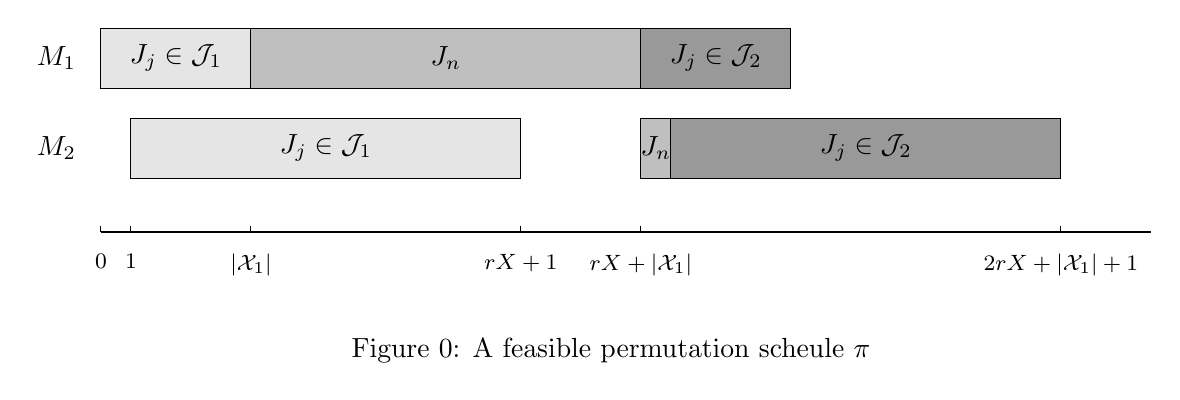
\begin{tikzpicture}[x=0.15in, y=0.3in]
                    
                    \node[anchor=east] at (-0.5,5.5) {$M_1$};
                    \node[anchor=east] at (-0.5,4) {$M_2$};
                    
                    \draw[fill=gray!20] (0,5)   rectangle (5,6)   node[midway] {$J_j \in \mathcal{J}_1$};
                    \draw[fill=gray!50] (5,5)   rectangle (18,6)   node[midway] {$J_n$};
                    \draw[fill=gray!80] (18,5)   rectangle (23,6)  node[midway] {$J_j \in \mathcal{J}_2$};
                    
                    \draw[fill=gray!20] (1,3.5)  rectangle (14,4.5)  node[midway] {$J_j \in \mathcal{J}_1$};
                    \draw[fill=gray!50] (18,3.5)  rectangle (19,4.5) node[midway] {$J_n$};
                    \draw[fill=gray!80] (19,3.5) rectangle (32,4.5)  node[midway] {$J_j \in \mathcal{J}_2$};
                    
                    \draw[thick] (0,2.6) -- (35,2.6);
                    \foreach \x/\label in {0/0, 1/1, 5/$|\mathcal{X}_1|$, 14/$rX+1$, 18/$rX +|\mathcal{X}_1|$, 32/$2rX+|\mathcal{X}_1|+1$}
                    {
                        \draw (\x,2.6) -- (\x,2.7);
                        \node[below, font=\footnotesize] at (\x,2.4) {\label};
                    }
                    
                    % caption
                    \node[below] at (17,1) {Figure~\thefigure: A feasible permutation scheule $\pi$};
                \end{tikzpicture}
                \label{fig:nphard-partition}
            \end{figure}
            
            Since $a_j \leq b_j$ for each $j=1, 2, \ldots, r$ and $|\mathcal{X}_1| \leq r-1$, it can be easily verified that $C_n(\pi)=rX +|\mathcal{X}_1|+1 \leq r(X+1)$ and $C_{\max}(\pi)=2rX+|\mathcal{X}_1|+1 \leq r(2X+1)$.
            Hence, $C_{\max}^w(\pi) \leq r(X+1)(2X+1)= Y$.
            
            Conversely, suppose that $F2 \mid \mid C_{\max}^w$ admits a feasible schedule $\pi$ with $C_{\max}^w(\pi) \leq Y$.
            Let $\mathcal{J}_1=\{J_j: C_j(\pi) <C_n(\pi)\}$ and $\mathcal{J}_2=\{J_j: C_j(\pi) > C_n(\pi)\}$ be the sets of jobs completed before and after $J_n$ in $\pi$, respectively, and let $\mathcal{X}_1=\{j: J_j \in \mathcal{J}_1\}$ and $\mathcal{X}_2=\{j: J_j \in \mathcal{J}_2\}$.
            By \cref{eq:completion}, we have
            \begin{equation}\label{eq:completetime1}
                C_n(\pi) \geq \sum_{j \in \mathcal{X}_1} a_j +a_n+ 1=|\mathcal{X}_1| +r X + 1
            \end{equation}
            and
            \begin{equation}\label{eq:completetime2}
                C_n(\pi) \geq a_{\pi(1)}+\sum_{j \in \mathcal{X}_1} b_j+b_n = r \sum_{j \in \mathcal{X}_1} x_j + 2.
            \end{equation}
            
            \textbf{Case 1.} If $\sum_{j \in \mathcal{X}_1} x_j > X$, then $\sum_{j \in \mathcal{X}_1} x_j \geq X+1$ because the $x_j$ are integers.
            By \cref{eq:completetime2}, $W C_{\max}(\pi) \geq w_n C_n(\pi) \geq (2X+1) (r(X+1)+2) >r(X+1)(2X+1)=Y$, contradicting the assumption that $C_{\max}^w(\pi) \leq Y$.
            
            \textbf{Case 2.} If $\sum_{j \in \mathcal{X}_1} x_j < X$, then $\sum_{j \in \mathcal{X}_1} x_j \leq X-1$ because the $x_j$ are integers.
            Since $(\mathcal{X}_1, \mathcal{X}_2)$ is a partition of $\{1, 2, \ldots, r\}$, we have
            \begin{equation} \label{eq:sum}
                \sum_{j \in \mathcal{X}_2} x_j =2X-\sum_{j \in \mathcal{X}_1} x_j \geq X+1.
            \end{equation}
            By \cref{eq:completion}, \cref{eq:completetime1}, and \cref{eq:sum}, we have
            \begin{equation}\label{eq:completetime3}
                C_{\pi(n)}(\pi)=C_{\max}(\pi) \geq C_n(\pi)+\sum_{j \in \mathcal{X}_2} b_j \geq |\mathcal{X}_1| +r X + 1+ r \sum_{j \in \mathcal{X}_2} x_j \geq r (2X + 1)+1.
            \end{equation}
            Using $w_{\pi(n)}=1$, \cref{eq:completetime3} yields
            \begin{equation*}
                C_{\max}^w(\pi) \geq w_{\pi(n)} C_{\pi(n)}(\pi) \geq (X+1) (r(2X+1)+1) >r(X+1)(2X+1)=Y,
            \end{equation*}
            This contradicts the assumption that $C_{\max}^w(\pi) \leq Y$.
            
            Combining the above two cases, we obtain that $\sum_{j \in \mathcal{X}_1} x_j = \sum_{j \in \mathcal{X}_2} x_j= X$.
            Therefore, $(\mathcal{X}_1, \mathcal{X}_2)$ is a solution to \textsc{Partition}.
        \end{proof}
        
        \begin{theorem}\label{thm:snphard}
            $F2 \mid \mid C_{\max}^w$ is strongly $\mathcal{NP}$-hard when $K$ is arbitrary.
        \end{theorem}
        \begin{proof}
            To establish the result, we give a polynomial-time reduction from 3-\textsc{Partition}, which is strongly  $\mathcal{NP}$-complete \citep{GareyJohnson1979computer}.
            
            3-\textsc{Partition}: Given $3r$ positive integers $x_1, x_2, \ldots, x_{3r}$ and an integer $X$ with $\sum_{i=1}^{3r}x_i=rX$ and $\frac{X}{4} < x_j < \frac{X}{2}$ for each $j=1, 2, \ldots, 3r$, does there exist a partition of $\{1, 2, \ldots, 3r\}$ into $m$ disjoint subsets $\mathcal{X}_1, \mathcal{X}_2, \ldots, \mathcal{X}_r$ such that $\sum_{j \in \mathcal{X}_i} x_j=X$ for $i=1, 2, \ldots, r$?
            
            Given an arbitrary instance $(x_1, x_2, \ldots, x_{3r}; X)$ of 3-\textsc{Partition}, we construct an instance of $F2 \mid \mid C_{\max}^w$ consisting of $r$ separating jobs and $3r$ basic jobs.
            For $j=1, 2, \ldots, r$, separating job $J_j$ has $a_j=4X$, $b_j=X$, and $w_j=\frac{5r+4}{5j}$; for $j=r+1, r+2, \ldots, 4r$, basic job $J_j$ has $a_j=x_{j-r}$, $b_j=4 x_{j-r}$, and $w_j=1$.
            Set the threshold to $Y=(5r+4)X$.
            The question is whether there exists a schedule with $W C_{\max} \leq Y$.
            
            We demonstrate that $F2 \mid \mid C_{\max}^w$ has a feasible schedule $\pi$ with $C_{\max}^w(\pi) \leq Y$ if and only if 3-\textsc{Partition} has a solution.
            
            Suppose that 3-\textsc{Partition} admits a solution $(\mathcal{X}_1, \mathcal{X}_2, \ldots, \mathcal{X}_r)$, so that $\sum_{j \in \mathcal{X}_i} x_j=X$ and $|\mathcal{X}_i|=3$ for all $i$.
            Let $\mathcal{J}_i=\{J_{r+j}: j \in \mathcal{X}_i\}$ for $i=1, 2, \ldots, r$.
            We build a feasible permutation schedule $\pi$ in which both machines process the jobs in the order
            \begin{equation*}
                J_1 \to \mathcal{J}_1 \to J_2 \to \mathcal{J}_2 \to \cdots \to J_r \to \mathcal{J}_r,
            \end{equation*}
            with the jobs in each $\mathcal{J}_i$ processed in arbitrary order (see \Cref{fig:nphard-3-partition}).
            
            \begin{figure}[H]
                \centering
                \refstepcounter{figure}
                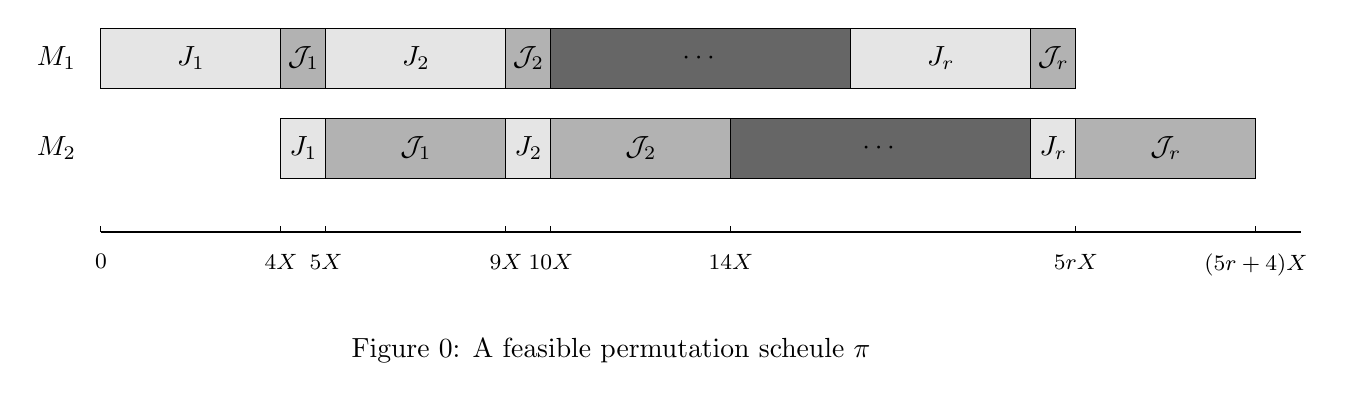
\begin{tikzpicture}[x=0.15in, y=0.3in]
                    
                    \node[anchor=east] at (-0.5,5.5) {$M_1$};
                    \node[anchor=east] at (-0.5,4) {$M_2$};
                    
                    \draw[fill=gray!20] (0,5)   rectangle (6,6)   node[midway] {$J_1$};
                    \draw[fill=gray!60] (6,5)   rectangle (7.5,6)   node[midway] {$\mathcal{J}_1$};
                    \draw[fill=gray!20] (7.5,5)   rectangle (13.5,6)  node[midway] {$J_2$};
                    \draw[fill=gray!60] (13.5,5)   rectangle (15,6)   node[midway] {$\mathcal{J}_2$};
                    \draw[fill=gray!120] (15,5)   rectangle (25,6)   node[midway] {$\cdots$};
                    \draw[fill=gray!20] (25,5)   rectangle (31,6)   node[midway] {$J_{r}$};
                    \draw[fill=gray!60] (31,5)   rectangle (32.5,6)   node[midway] {$\mathcal{J}_r$};
                    
                    \draw[fill=gray!20] (6,3.5)  rectangle (7.5,4.5)  node[midway] {$J_1$};
                    \draw[fill=gray!60] (7.5,3.5)  rectangle (13.5,4.5) node[midway] {$\mathcal{J}_1$};
                    \draw[fill=gray!20] (13.5,3.5) rectangle (15,4.5)  node[midway] {$J_2$};
                    \draw[fill=gray!60] (15,3.5)  rectangle (21,4.5) node[midway] {$\mathcal{J}_2$};
                    \draw[fill=gray!120] (21,3.5)  rectangle (31,4.5) node[midway] {$\cdots$};
                    \draw[fill=gray!20] (31,3.5) rectangle (32.5,4.5)  node[midway] {$J_r$};
                    \draw[fill=gray!60] (32.5,3.5)  rectangle (38.5,4.5) node[midway] {$\mathcal{J}_r$};
                    
                    \draw[thick] (0,2.6) -- (40,2.6);
                    \foreach \x/\label in {0/0, 6/$4X$, 7.5/$5X$, 13.5/$9X$, 15/$10X$, 21/$14X$, 32.5/$5rX$, 38.5/$(5r+4)X$}
                    {
                        \draw (\x,2.6) -- (\x,2.7);
                        \node[below, font=\footnotesize] at (\x,2.4) {\label};
                    }
                    
                    % caption
                    \node[below] at (17,1) {Figure~\thefigure: A feasible permutation scheule $\pi$};
                \end{tikzpicture}
                \label{fig:nphard-3-partition}
            \end{figure}
            
            According to \Cref{fig:nphard-3-partition}, it can be easily verified that $C_j(\pi)=5jX$ for $j=1, 2, \ldots, r$, and $C_j(\pi) \leq C_{\max}(\pi)=(5r+4)X$ for $j=r+1, r+2, \ldots, 4r$.
            Then $w_j C_j(\pi)=(5r+4)X=Y$ for $j=1, 2, \ldots, r$, and $w_j C_j(\pi) \leq w_j C_{\max}(\pi)=(5r+4)X=Y$ for $j=r+1, r+2, \ldots, 4r$.
            Hence, $C_{\max}^w(\pi) \leq Y$.
            
            Conversely, suppose that $F2 \mid \mid C_{\max}^w$ admits a feasible schedule $\pi$ with $C_{\max}^w(\pi) \leq Y$.
            Because all separating jobs have the same processing time on $M_1$ and $M_2$ and weights $w_1 >w_2 > \cdots > w_r$, a standard interchange argument lets us assume they appear in $\pi$ in decreasing order of weight.
            
            \textbf{Claim 1.} $C_{\max}(\pi) \leq Y=(5r+4)X$.
            
            \textit{Proof of Claim 1.}  Since $w_j \geq 1$ for all $1 \leq j \leq 4r$, we have $C_{\max}(\pi) \leq C_{\max}^w(\pi) \leq Y=(5r+4)X$.
            \hfill$\blacksquare$
            
            \textbf{Claim 2.} $J_1$ is the first job scheduled in $\pi$.
            
            \textit{Proof of Claim 2.}  Since $C_{\max}^w(\pi) \leq Y=(5r+4)X$ and $w_1=\frac{5r+4}{5}$, we have $a_1+b_1 \leq C_1(\pi) \leq \frac{C_{\max}^w(\pi)}{w_1} \leq 5X=a_1+b_1$.
            This means that $J_1$ is the first job scheduled in $\pi$.
            \hfill$\blacksquare$
            
            For $i=1, 2, \ldots, r-1$, let $\mathcal{B}_i=\{J_j: C_i(\pi) < C_j(\pi) < C_{i+1}(\pi)\}$ be the set of basic jobs scheduled between $J_i$ and $J_{i+1}$ in $\pi$, and let $\mathcal{B}_r=\{J_j: C_j(\pi) > C_r(\pi)\}$ be the set of basic jobs scheduled after $J_r$.
            For $i=1, 2, \ldots, r$, define $\mathcal{X}_i=\{j-r: J_j \in  \mathcal{B}_i\}$.
            Then, by Claim 2, $\pi$ can be written as
            \begin{equation} \label{eq:order}
                \pi=(J_1 \to \mathcal{B}_1 \to J_2 \to \mathcal{B}_2 \to \cdots \to J_r \to \mathcal{B}_r).
            \end{equation}
            
            Since $(\mathcal{X}_1, \mathcal{X}_2, \ldots, \mathcal{X}_r)$ is a partition of $\{1, 2, \ldots, 3r\}$, we have
            \begin{equation} \label{eq:00}
                \sum_{i=1}^r \sum_{j \in \mathcal{X}_i} x_j =\sum_{j=1}^{3r} x_j =rX.
            \end{equation}
            
            \textbf{Claim 3.} For $k=1, 2, \ldots, r-1$, $\sum_{i=1}^k \sum_{j \in \mathcal{X}_i} x_j \leq kX$.
            
            \textit{Proof of Claim 3.} Suppose to the contrary that there exists some $m$ ($1 \leq m \leq r-1$) with $\sum_{i=1}^m \sum_{j \in \mathcal{X}_i} x_j > mX$.
            Since the $x_j$ are integers, this implies
            \begin{equation}\label{eq:10}
                \sum_{i=1}^m \sum_{j \in \mathcal{X}_i} x_j \geq mX+1.
            \end{equation}
            Because $a_j=4X$ and $b_j=X$ for $1 \leq j \leq r$, and $a_j=x_{j-r}$ for $r+1 \leq j \leq 4r$, \cref{eq:completion}, \cref{eq:order}, and \cref{eq:10} give
            \begin{equation} \label{eq:11}
                C_{m+1}(\pi) \geq \sum_{j=1}^{m+1} a_j+\sum_{i=1}^m \sum_{j \in \mathcal{B}_i} a_j+b_{m+1} =4(m+1)X+\sum_{i=1}^m \sum_{j \in \mathcal{X}_i} x_j +X \geq 5(m+1)X+1.
            \end{equation}
            Using $w_{m+1}=\frac{5r+4}{5(m+1)}$, \cref{eq:11} yields
            \begin{equation} \label{eq:12}
                C_{\max}^w(\pi) \geq w_{m+1} C_{m+1}(\pi) \geq \frac{5r+4}{5(m+1)} (5(m+1)X+1)>(5r+4)X=Y,
            \end{equation}
            which contradicts the assumption that $C_{\max}^w(\pi) \leq Y$.
            Hence, Claim 3 holds.
            \hfill$\blacksquare$
            
            \textbf{Claim 4.} For $k=1, 2, \ldots, r-1$, $\sum_{i=1}^k \sum_{j \in \mathcal{X}_i} x_j \geq kX$.
            
            \textit{Proof of Claim 4.} Suppose to the contrary that there exists some $m$ ($1 \leq m \leq r-1$) with $\sum_{i=1}^m \sum_{j \in \mathcal{X}_i} x_j < mX$.
            By \cref{eq:00} and the $x_j$ are integers, we have
            \begin{equation}\label{eq:20}
                \sum_{i=m+1}^r \sum_{j \in \mathcal{X}_i} x_j=rX-\sum_{i=1}^m \sum_{j \in \mathcal{X}_i} x_j \geq (r-m)X+1.
            \end{equation}
            Because $a_j=4X$ and $b_j=X$ for $1 \leq j \leq r$, and $a_j=x_{j-r}$ and $b_j=4 x_{j-r}$ for $r+1 \leq j \leq 4r$, \cref{eq:completion}, \cref{eq:order}, \cref{eq:00}, and \cref{eq:20} give
            \begin{align*}
                C_{\max}(\pi) & \geq \sum_{j=1}^{m+1} a_j+\sum_{i=1}^m \sum_{j \in \mathcal{B}_i} a_j+\sum_{j=m+1}^r      b_j+\sum_{i=m+1}^r \sum_{j \in \mathcal{B}_i} b_j  \nonumber \\
                &= 4(m+1)X+\sum_{i=1}^m \sum_{j \in \mathcal{X}_i} x_j +(r-m)X +\sum_{i=m+1}^r \sum_{j \in \mathcal{X}_i} 4 x_j \nonumber \\
                &= 4(m+1)X +(r-m)X + rX+ 3 \sum_{i=m+1}^r \sum_{j \in \mathcal{X}_i} x_j \\
                & \geq 4(m+1)X +(r-m)X + rX+ 3((r-m)X+1)  \nonumber \\
                & = (5r+4)X +3 > (5r+4)X = Y. \nonumber
            \end{align*}
            which contradicts Claim 1.
            Hence, Claim 4 holds.
            \hfill$\blacksquare$
            
            Combining Claims 3 and 4 with \cref{eq:00}, we obtain that $\sum_{j \in \mathcal{X}_i} x_j=X$ for $i=1, 2, \ldots, r$.
            Since $X/4 < x_j < X/2$ for each $j$, a sum equal to $X$ must contain exactly three elements; hence  $|\mathcal{X}_i|=3$ for each $i$.
            Therefore, $(\mathcal{X}_1, \mathcal{X}_2, \ldots, \mathcal{X}_r)$ is a solution to 3-\textsc{Partition}.
        \end{proof}
        
        \section{Fixed number of weights} \label{sec:dp_algorithm}
        
        In this section, we focus on the case where the number of weights $K$ is fixed, i.e., $K=O(1)$.
        For $K=1$, the problem is exactly $F2 \mid \mid C_{\max}$, which Johnson's rule solves in $O(n \log n)$ time \citep{Johnson1954NRL}; the rule is summarized in \Cref{alg:Johnson}.
        For $K=2$, the problem $F2 \mid \mid C_{\max}^w$ is already binary $\mathcal{NP}$-hard (\Cref{thm:nphard}).
        For fixed $K$, we develop an exact DP algorithm running in pseudo-polynomial time and derive an FPTAS from it.
        
        \begin{algorithm}[H]
            \small
            \SetAlgoLined
            \DontPrintSemicolon
            \caption{Johnson's rule for $F2\mid\mid C_{\max}$}\label{alg:Johnson}
            \KwIn{Job set $\mathcal{J}$; job parameters $a_j$ and $b_j$ for $j=1, 2, \ldots, n$.}
            \BlankLine
            \textbf{Step 1.} Partition $\mathcal{J}$ into two sets $\mathcal{J}^1=\{J_j: a_j \leq b_j\}$
            and $\mathcal{J}^2=\{J_j: a_j>b_j\}$.
            
            \textbf{Step 2.} Order the jobs in $\mathcal{J}^1$ in nondecreasing order of $a_j$, followed by those in $\mathcal{J}^2$ in nondecreasing order of $b_j$. \;
            
            \textbf{Step 3.} Process the jobs in this order on $M_1$ and then on $M_2$, yielding the permutation schedule $\pi$. \;
            
            \KwOut{The resulting schedule $\pi$.}
        \end{algorithm}
        
        Let $W_1 > W_2 > \cdots > W_K$ denote the distinct weights of the $n$ jobs, and let $\mathcal{G}_k = \{J_j \in \mathcal{J}: w_j = W_k\}$ be set of jobs having weight $W_k$, $k=1, 2,\ldots, K$.
        
        \subsection{Block structure of an optimal schedule} \label{sec:block}
        
        To establish the key structural lemma, we first introduce some notation for partitioning a permutation schedule into blocks.
        \begin{definition} \label{def:block}
            \textbf{(Block partition)} Let $\pi = (\pi(1), \pi(2), \ldots, \pi(n))$ be a permutation schedule.
            Set $\ell_0 = 0$ and $\mathcal{R}_1=\mathcal{J}$.
            For $k = 1, 2, \ldots, K$, if $\mathcal{R}_k \cap \mathcal{G}_k \neq \emptyset$, define $\ell_k=\max \{j: J_{\pi(j)} \in \mathcal{R}_k \cap \mathcal{G}_k\}$, $\mathcal{B}_k^{\pi} = \{J_{\pi(\ell_{k-1}+1)}, J_{\pi(\ell_{k-1}+2)}, \ldots, J_{\pi(\ell_k)}\}$, and $\mathcal{R}_{k+1}=\mathcal{J}\setminus\bigcup_{i=1}^{k}\mathcal{B}_i^{\pi}$.
            Otherwise, set $\ell_k=\ell_{k-1}$,  $\mathcal{B}_k^{\pi} =\emptyset$, and $\mathcal{R}_{k+1}=\mathcal{R}_{k}$.
            Then we call $\mathcal{B}(\pi)=(\mathcal{B}_1^{\pi}, \mathcal{B}_2^{\pi}, \ldots, \mathcal{B}_K^{\pi})$ the block partition of $\pi$.
        \end{definition}
        
        Thus, $\ell_k$ is the position of the last job in $\mathcal{R}_k$ of weight $W_k$, $\mathcal{B}_k^{\pi}$ is the $k$-th block (possibly empty), and $\mathcal{R}_k$ is the set of jobs left after removing the first $k-1$ blocks.
        By construction, every nonempty block $\mathcal{B}_k^{\pi}$ ends with a job of weight $W_k$ (i.e., $w_{\pi(\ell_k)}=W_k$), and all jobs in the block have weight at most $W_k$, i.e., $w_{\pi(j)} \leq W_k$ for all  $\ell_{k-1}+1 \leq j \leq \ell_{k}$.
        This means that
        \begin{equation} \label{eq:block-1}
            W_k C_{\pi(\ell_k)}(\pi)=\max \{w_{\pi(j)} C_{\pi(j)}(\pi): \ell_{k-1}+1 \leq j \leq \ell_{k}\}.
        \end{equation}
        Consequently, \cref{eq:wcmax} can be reformulated as
        \begin{equation}\label{eq:block-comp}
            C_{\max}^w(\pi)=\max_{1 \leq k \leq K} \{W_k C_{\pi(\ell_k)(\pi)}\}.
        \end{equation}
        
        \begin{definition}\label{def:regular}
            \textbf{(Regular block and regular permutation schedule)} Let $\pi=(\pi(1),\pi(2),\ldots,\pi(n))$ be a permutation schedule with block partition $\mathcal{B}(\pi)=(\mathcal{B}_1^{\pi},\mathcal{B}_2^{\pi},\ldots,\mathcal{B}_K^{\pi})$.
            A block $\mathcal{B}_k^{\pi}$ is called regular if it is empty or if the sequence of its jobs in $\pi$ matches the sequence obtained by applying Johnson's rule to that block.
            The schedule $\pi$ is called regular if all blocks  $\mathcal{B}_1^{\pi},\mathcal{B}_2^{\pi},\ldots,\mathcal{B}_K^{\pi}$ are regular.
        \end{definition}
        
        To illustrate the block partition, we give a small numerical example for $F2 \mid \mid C_{\max}^w$.
        
        \begin{exam}\label{ex:blocking}
            Consider a six-job instance of $F2 \mid \mid C_{\max}^w$ whose job data are given in \Cref{tab:TA-2-1}, and let $\pi = (1, 2, \ldots, 6)$ be a permutation schedule.
        \end{exam}
        \begin{table}[htbp]
            \small
            \centering
            \caption{Job data for \Cref{ex:blocking}}   \label{tab:TA-2-1}
            \begin{tabular}{c|cccccc}
                & $J_1$ & $J_2$ & $J_3$ & $J_4$ & $J_5$ & $J_6$ \\
                \hline
                $a_j$ & 2 & 5 & 6 & 8 & 2 & 3 \\
                $b_j$ & 5 & 3 & 9 & 4 & 3 & 3 \\
                $w_j$ & 2 & 3 & 5 & 2 & 3 & 2 \\
            \end{tabular}
        \end{table}
        
        In \Cref{ex:blocking}, we have $K=3$, $\mathcal{G}_1=\{J_3\}$, $\mathcal{G}_2=\{J_2, J_5\}$, and $\mathcal{G}_3=\{J_1,J_4,J_6\}$.
        The resulting blocks are $\mathcal{B}_1^{\pi}=\{J_1,J_2,J_3\}$, $\mathcal{B}_2^{\pi}=\{J_4,J_5\}$, and $\mathcal{B}_3^{\pi}=\{J_6\}$ (see \Cref{fig:exam}).
        By \cref{eq:block-comp}, the weighted makespan of $\pi$ is $C_{\max}^w(\pi)=\max \{5 \times 22, 3 \times 29, 2 \times 32\}=110$.
        
        \begin{figure}[H]
            \centering
            \refstepcounter{figure}
            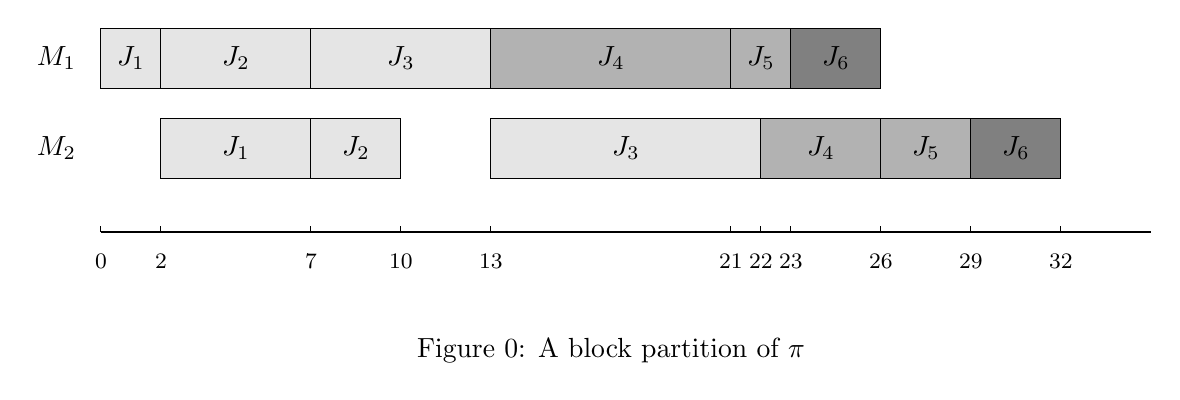
\begin{tikzpicture}[x=0.15in, y=0.3in]
                % machine index
                \node[anchor=east] at (-0.5,5.5) {$M_1$};
                \node[anchor=east] at (-0.5,4) {$M_2$};
                
                \draw[fill=gray!20] (0,5)   rectangle (2,6)   node[midway] {$J_1$};
                \draw[fill=gray!20] (2,5)   rectangle (7,6)   node[midway] {$J_2$};
                \draw[fill=gray!20] (7,5)   rectangle (13,6)  node[midway] {$J_3$};
                \draw[fill=gray!60] (13,5)  rectangle (21,6)  node[midway] {$J_4$};
                \draw[fill=gray!60] (21,5)  rectangle (23,6)  node[midway] {$J_5$};
                \draw[fill=gray!100] (23,5)  rectangle (26,6)  node[midway] {$J_6$};
                
                \draw[fill=gray!20] (2,3.5)  rectangle (7,4.5)  node[midway] {$J_1$};
                \draw[fill=gray!20] (7,3.5)  rectangle (10,4.5) node[midway] {$J_2$};
                \draw[fill=gray!20] (13,3.5) rectangle (22,4.5) node[midway] {$J_3$};
                \draw[fill=gray!60] (22,3.5) rectangle (26,4.5) node[midway] {$J_4$};
                \draw[fill=gray!60] (26,3.5) rectangle (29,4.5) node[midway] {$J_5$};
                \draw[fill=gray!100] (29,3.5) rectangle (32,4.5) node[midway] {$J_6$};
                
                % x-axis
                \draw[thick] (0,2.6) -- (35,2.6);
                \foreach \x/\label in {0/0, 2/2, 7/7, 10/10, 13/13, 21/21, 22/22, 23/23, 26/26, 29/29, 32/32} {
                    \draw (\x,2.6) -- (\x,2.7);
                    \node[below, font=\footnotesize] at (\x,2.4) {\label};
                }
                
                % caption
                \node[below] at (17,1) {Figure~\thefigure: A block partition of $\pi$};    \label{fig:exam}
            \end{tikzpicture}
        \end{figure}
        
        Given a permutation schedule $\pi=(\pi(1), \pi(2), \ldots, \pi(n))$, for $1 \leq g \leq h \leq n$, define \begin{equation*}
            C_{\max}^w(\pi)[g:h]= \max_{g \leq j \leq h}\{w_{\pi(j)}C_{\pi(j)}(\pi)\}
        \end{equation*}
        as the maximum weighted completion time over the jobs $J_{\pi(g)}, J_{\pi(g+1)}, \ldots, J_{\pi(h)}$.
        
        The following lemma shows that if the jobs in each block of $\pi$ are rescheduled in accordance with Johnson's rule, the resulting permutation schedule $\pi'$ has objective value no larger than that of $\pi$, i.e., $C_{\max}^w(\pi') \leq C_{\max}^w(\pi)$.
        
        \begin{lemma}\label{lem:block-johnson}
            Given a permutation schedule $\pi$ and its block partition $\mathcal{B}(\pi)=(\mathcal{B}_1^{\pi}, \mathcal{B}_2^{\pi}, \ldots, \mathcal{B}_K^{\pi})$, let $\pi_k$ be the permutation of $\mathcal{B}_k^{\pi}$ obtained by Johnson's rule for $k=1, 2, \ldots, K$.
            Then the schedule $\pi'$ formed by concatenating $\pi_1, \pi_2, \ldots, \pi_K$ satisfies  $C_{\max}^w(\pi') \leq C_{\max}^w(\pi)$.
        \end{lemma}
        
        \begin{proof}
            First, if $\mathcal{B}_k^{\pi} \neq \emptyset$, then rescheduling the jobs in $\mathcal{B}_k^{\pi}$ according to Johnson's rule does not change the set of jobs assigned to positions $\ell_{k-1}+1, \ell_{k-1}+2, \ldots, \ell_k$, i.e.,
            \begin{equation} \label{eq:induc-1}
                \mathcal{B}_k^{\pi} = \{J_{\pi(\ell_{k-1}+1)}, J_{\pi(\ell_{k-1}+2)}, \ldots, J_{\pi(\ell_k)}\}=\{J_{\pi'(\ell_{k-1}+1)}, J_{\pi'(\ell_{k-1}+2)}, \ldots, J_{\pi'(\ell_k)}\}.
            \end{equation}
            Thus, in $\pi'$, the jobs in $\mathcal{B}_k^{\pi}$ still occupy this same index interval.
            By \cref{eq:block-1}, we have
            \begin{equation}  \label{eq:induc-2}
                C_{\max}^w(\pi)[\ell_{k-1}+1:\ell_k]=W_k C_{\pi(\ell_k)}(\pi)=w_{\pi(\ell_k)} C_{\pi(\ell_k)}(\pi), k=1, 2, \ldots, K.
            \end{equation}
            Moreover, by \cref{eq:induc-1}, for $k=1, 2, \ldots, K$, $\mathcal{B}_k^{\pi}$ has the same completion time on $M_1$ under $\pi$ and $\pi'$, i.e., $C_{\pi'(\ell_k)}^1(\pi')=C_{\pi(\ell_k)}^1(\pi)=\sum_{j=1}^{\ell_k} a_{\pi(j)}$.
            
            Second, we prove by induction on $k$ that, for all $k=1, 2, \ldots, K$,
            \begin{equation} \label{eq:induc-assump}
                C_{\pi'(\ell_k)} (\pi') \leq C_{\pi(\ell_k)}(\pi) ~ \mathrm{and}  ~ C_{\max}^w(\pi')[\ell_{k-1}+1:\ell_k] \leq C_{\max}^w(\pi)[\ell_{k-1}+1:\ell_k].
            \end{equation}
            
            For the base case $i=1$, both machines are available at time zero.
            Rescheduling the jobs in $\mathcal{B}_1^{\pi}$ according to Johnson's rule gives $C_{\pi'(\ell_1)}(\pi') \leq C_{\pi(\ell_1)}(\pi)$.
            Since $\pi'$ only permutes the jobs in $\mathcal{B}_1^{\pi}$, we have $w_{\pi'(j)} \leq W_1$ for $j=1, 2, \ldots, \ell_1$.
            Hence, we have
            \begin{equation*}
                C_{\max}^w(\pi')[1:\ell_1]= \max_{1 \leq j \leq \ell_1}\{w_{\pi'(j)}C_{\pi'(j)}(\pi')\} \leq W_1 C_{\pi'(\ell_1)}(\pi') \leq W_1 C_{\pi(\ell_1)}(\pi)=C_{\max}^w(\pi)[1:\ell_1],
            \end{equation*}
            where the last equality follows from \cref{eq:induc-2}
            
            Assume that \cref{eq:induc-assump} holds for all $i=1, 2, \ldots, k$.
            We now prove the $(k+1)$-block.
            If $\mathcal{B}_{k+1}^{\pi}=\emptyset$, the assertion is immediate.
            It remains to consider $\mathcal{B}_{k+1}^{\pi} \neq \emptyset$.
            In this case, in $\pi'$, by the inductive hypothesis, $M_1$ becomes available at time $C_{\pi'(\ell_k)}^1(\pi')=C_{\pi(\ell_k)}^1(\pi)$, and $M_2$ is available at time $C_{\pi'(\ell_k)}(\pi') \leq C_{\pi(\ell_k)}(\pi)$.
            We introduce a dummy job $J_0$ with processing times $a_0=0$ and $b_0=C_{\pi'(\ell_k)}(\pi')-C_{\pi'(\ell_k)}^1(\pi')$, and apply Johnson's rule to schedule the jobs in $\mathcal{B}_{k+1}^{\pi} \cup \{J_0\}$, with both machines available from time $C_{\pi'(\ell_k)}^1(\pi')$.
            Because $a_0=0$, $J_0$ is scheduled in the first position according to Johnson's rule, and it completes at time $C_{\pi'(\ell_k)}(\pi')$.
            By positioning the dummy job in this way, the jobs in $\mathcal{B}_{k+1}^{\pi}$ can be scheduled on $M_2$ without overlapping with the previously scheduled jobs in $\mathcal{B}_1^{\pi} \cup \mathcal{B}_2^{\pi} \cup \cdots \cup \mathcal{B}_k^{\pi}$.
            Since the jobs in $\mathcal{B}_{k+1}$ are scheduled according to Johnson's rule, it follows that $C_{\pi'(\ell_{k+1})} (\pi') \leq C_{\pi(\ell_{k+1})}(\pi)$.
            Moreover, since $\pi'$ only permutes the jobs in $\mathcal{B}_{k+1}^{\pi}$, we have $w_{\pi'(j)} \leq W_{k+1}$ for $j=\ell_k+1, \ell_k+2, \ldots, \ell_{k+1}$.
            Hence,
            \begin{align*}
                C_{\max}^w(\pi')[\ell_k+1:\ell_{k+1}] & = \max_{\ell_k+1 \leq j \leq \ell_{k+1}}\{w_{\pi'(j)}C_{\pi'(j)}(\pi')\} \leq W_{k+1} C_{\pi'(\ell_{k+1})}(\pi') \\
                & \leq W_{k+1} C_{\pi(\ell_{k+1})}(\pi)=C_{\max}^w(\pi)[\ell_k+1:\ell_{k+1}],
            \end{align*}
            where the last equality follows from \cref{eq:induc-2}.
            This completes the inductive step.
            
            Note that $C_{\max}^w(\pi')=\max\limits_{1 \leq k \leq K} \{C_{\max}^w(\pi')[\ell_{k-1}+1:\ell_k]\}$ and $C_{\max}^w(\pi)=\max\limits_{1 \leq k \leq K} \{C_{\max}^w(\pi)[\ell_{k-1}+1:\ell_k]\}$.
            Hence, \cref{eq:induc-assump} yields $C_{\max}^w(\pi') \leq C_{\max}^w(\pi)$.
        \end{proof}
        
        To illustrate \Cref{lem:block-johnson}, consider \Cref{ex:blocking}.
        Given $\pi$ and its block partition $\mathcal{B}(\pi)=(\mathcal{B}_1^{\pi}, \mathcal{B}_2^{\pi}, \mathcal{B}_3^{\pi})$, we apply Johnson’s rule independently within each block $\mathcal{B}_k^{\pi}$, $k=1, 2, 3$, obtaining a permutation $\pi_k$ of the jobs in that block.
        Concatenating $\pi_1, \pi_2, \pi_3$ gives $\pi'=(1, 3, 2, 5, 4, 6)$, with blocks $\mathcal{B}_1^{\pi'}=\{J_1,J_3\}$, $\mathcal{B}_2^{\pi'}=\{J_2,J_5\}$, and $\mathcal{B}_3^{\pi'}=\{J_4, J_6\}$ (see \Cref{fig:exam-2}).
        By \cref{eq:block-comp}, the weighted makespan of $\pi'$ is $C_{\max}^w(\pi')=\max \{5 \times 17, 3 \times 23, 2 \times 30\}=85$.
        
        \begin{figure}[H]
            \centering
            \refstepcounter{figure}
            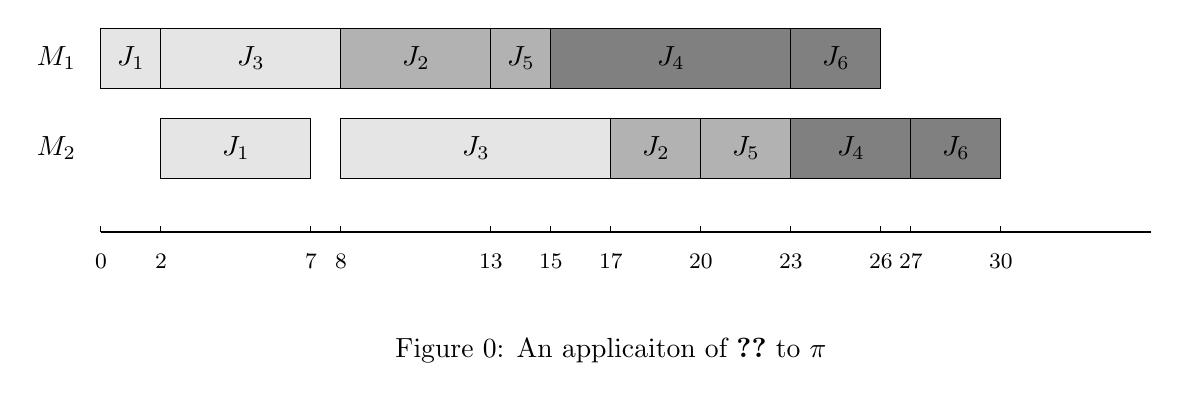
\begin{tikzpicture}[x=0.15in, y=0.3in]
                % machine index
                \node[anchor=east] at (-0.5,5.5) {$M_1$};
                \node[anchor=east] at (-0.5,4) {$M_2$};
                
                \draw[fill=gray!20] (0,5)   rectangle (2,6)   node[midway] {$J_1$};
                \draw[fill=gray!20] (2,5)   rectangle (8,6)   node[midway] {$J_3$};
                \draw[fill=gray!60] (8,5)   rectangle (13,6)  node[midway] {$J_2$};
                \draw[fill=gray!60] (13,5)  rectangle (15,6)  node[midway] {$J_5$};
                \draw[fill=gray!100] (15,5)  rectangle (23,6)  node[midway] {$J_4$};
                \draw[fill=gray!100] (23,5)  rectangle (26,6)  node[midway] {$J_6$};
                
                \draw[fill=gray!20] (2,3.5)  rectangle (7,4.5)  node[midway] {$J_1$};
                \draw[fill=gray!20] (8,3.5)  rectangle (17,4.5) node[midway] {$J_3$};
                \draw[fill=gray!60] (17,3.5) rectangle (20,4.5) node[midway] {$J_2$};
                \draw[fill=gray!60] (20,3.5) rectangle (23,4.5) node[midway] {$J_5$};
                \draw[fill=gray!100] (23,3.5) rectangle (27,4.5) node[midway] {$J_4$};
                \draw[fill=gray!100] (27,3.5) rectangle (30,4.5) node[midway] {$J_6$};
                
                % x-axis
                \draw[thick] (0,2.6) -- (35,2.6);
                \foreach \x/\label in {0/0, 2/2, 7/7, 8/8, 13/13, 15/15, 17/17, 20/20, 23/23, 26/26, 27/27, 30/30} {
                    \draw (\x,2.6) -- (\x,2.7);
                    \node[below, font=\footnotesize] at (\x,2.4) {\label};
                }
                
                % caption
                \node[below] at (17,1) {Figure~\thefigure: An applicaiton of \Cref{lem:block-johnson} to $\pi$};    \label{fig:exam-2}
            \end{tikzpicture}
        \end{figure}
        
        \begin{lemma}\label{lem:regular-schedule}
            For $F2 \mid \mid C_{\max}^w$, there exists an optimal permutation schedule that is regular.
        \end{lemma}
        
        \begin{proof}
            Let $\pi$ be an optimal permutation schedule for $F2 \mid \mid C_{\max}^w$.
            If $\pi$ is regular, the lemma follows.
            Otherwise, let $\mathcal{B}(\pi)=(\mathcal{B}_1^{\pi}, \mathcal{B}_2^{\pi}, \ldots, \mathcal{B}_K^{\pi})$ be its block partition.
            Apply Johnson’s rule within each block $\mathcal{B}_k^{\pi}$ ($k=1, 2, \ldots, K$) to obtain a permutation $\pi_k$, and concatenate $\pi_1, \pi_2, \ldots, \pi_K$ to form a permutation schedule $\pi'$.
            By \Cref{lem:block-johnson}, $C_{\max}^w(\pi') \leq C_{\max}^w(\pi)$.
            Since $\pi$ is optimal, $\pi'$ is optimal as well.
            
            If $\pi'$ is regular, the lemma follows.
            Otherwise, repeat the above procedure with $\pi'$ in place of $\pi$.
            For termination, suppose the first $i$ blocks of the current schedule are already regular (initially $i=0$).
            By definition, applying Johnson's rule to a regular block leaves its job sequence unchanged.
            Hence, the first $i$ blocks remain unchanged.
            The $(i+1)$-th block in the resulting schedule may contain a different job set, but it satisfies Johnson's rule.
            Thus the first $i+1$ blocks are regular, so every application increases the number of leading regular blocks by at least one.
            Since there are at most $K$ nonempty blocks in each schedule, the procedure terminates after at most $K$ iterations and yields an optimal regular schedule.
        \end{proof}
        
        Let $\pi$ be a regular permutation schedule for $F2 \mid \mid C_{\max}^w$ with block partition $\mathcal{B}(\pi)=(\mathcal{B}_1^{\pi}, \mathcal{B}_2^{\pi}, \ldots, \mathcal{B}_K^{\pi})$.
        For each $k=1, 2, \ldots, K$, let $\pi_k$ denote the schedule obtained by processing the jobs in $\mathcal{B}_k^{\pi}$ consecutively from time zero in accordance with Johnson’s rule.
        Note that $\pi$ coincides with the schedule obtained by concatenating $\pi_1, \pi_2, \ldots, \pi_K$.
        This representation allows us to compute $C_{\max}(\pi)$ and $C_{\max}^w(\pi)$ from parameters defined for each $\pi_k$.
        Specifically, for each $k$, let $A_k=A(\pi_k)$ and $B_k=B(\pi_k)$ denote the total processing times of the jobs in $\pi_k$ on $M_1$ and $M_2$, respectively, and let $C_k=C(\pi_k)$ denote the makespan of $\pi_k$.
        Given these parameters, we describe an procedure for computing $C_{\max}(\pi)$ and $C_{\max}^w(\pi)$.
        The procedure starts with $\pi_1$ and successively appends $\pi_2, \pi_3, \ldots, \pi_K$ in that order.
        For $k=1, 2, \ldots, K$, let $\pi[1:k]$ denote the schedule obtained by concatenating $\pi_1, \pi_2, \ldots, \pi_k$; thus $\pi=\pi[1:K]$.
        The makespan and weighted makespan of $\pi[1: k]$ are computed recursively.
        For convenience, set $C_{\max}(\pi[1: 0])=C_{\max}^w(\pi[1: 0])=0$.
        For $k=1, 2, \ldots, K$, by direct calculation and induction on $k$, we have
        \begin{equation}
            \begin{aligned} \label{eq-4.2:block-makespan}
                C_{\max}(\pi[1: k]) &=\max \Big\{\sum_{i=1}^{k-1} A_i+C_k, C_{\max}(\pi[1: k-1])+B_k\Big\}  \\
                &= \max_{0 \leq h \leq k-1} \Big\{ \sum_{i=1}^h A_i +C_{h+1} + \sum_{i=h+2}^k B_i \Big\}
            \end{aligned}
        \end{equation}
        and
        \begin{equation}\label{eq-4.2:block-weighted makespan}
            \begin{aligned}
                C_{\max}^w(\pi[1: k]) &=\max \{C_{\max}^w(\pi[1: k-1]), W_k C_{\max}(\pi[1: k])\}  \\
                &= \max_{1 \leq h \leq k} \{W_h C_{\max}(\pi[1: h])\}.
            \end{aligned}
        \end{equation}
        Hence, $C_{\max}^w(\pi)=C_{\max}^w(\pi[1: K])$.
        
        \subsection{An exact DP algorithm} \label{sec:dp}
        
        Recall that $W_1 >W_2 > \cdots W_K$.
        For each job $J_j$ ($j=1, 2, \ldots, n$), let $g_j \in \{1, 2, \ldots, K\}$ be the index such that $w_j=W_{g_j}$, i.e., $J_j\in\mathcal{G}_{g_j}$.
        Assume that the jobs in $\mathcal{J}$ are indexed in accordance with Johnson's rule.
        
        Building on the preceding discussion in \Cref{sec:block}, we develop an exact DP algorithm for $F2 \mid \mid C_{\max}^w$.
        It generates a sequence of sets $\mathcal{H}_0, \mathcal{H}_1, \ldots, \mathcal{H}_n$.
        Each $\mathcal{H}_j$ consists of $K$-tuples $(X_1, X_2, \ldots, X_K)$, where $X_k=(A_k, B_k, C_k, L_k)$ for $k=1, 2, \ldots, K$.
        A tuple in $\mathcal{H}_j$ ($j=1, 2, \ldots, n$) encodes an assignment of jobs $J_1, J_2, \ldots, J_j$ to $K$ schedules (i.e., blocks) $\pi_1(j), \pi_2(j), \ldots, \pi_K(j)$, with jobs in each schedule processed from time zero in increasing order of their indices.
        For each schedule $\pi_k(j)$, $A_k$ and $B_k$ are the total processing times on $M_1$ and $M_2$, respectively, and $C_k$ and $L_k$ are the makespan of $\pi_k(j)$ and the weight of its last job.
        
        Initially, $\mathcal{H}_0$ consists of a single tuple, all of whose $4K$ entries are zero, i.e., $\mathcal{H}_0=\{\Big (\underbrace{(0,0,0,0),\ldots,(0,0,0,0)}_{K\text{ copies}}\Big)\}$.
        In the $j$-th iteration ($j=1, 2, \ldots, n$), $\mathcal{H}_j$ is constructed from $\mathcal{H}_{j-1}$.
        For each tuple $(X_1, X_2, \ldots, X_K) \in \mathcal{H}_{j-1}$, with $X_k=(A_k, B_k, C_k, L_k)$ for $k=1, 2, \ldots, K$, the definition of $g_j$ and \Cref{lem:regular-schedule} together imply that this tuple generates $g_j$ new tuples in $\mathcal{H}_j$.
        If $k \leq g_j$, appending $J_j$ to $\pi_k(j-1)$ yields the new tuple $(X_1, \ldots, X_{k-1}, X'_k, X_{k+1}, \ldots, X_K)$ into $\mathcal{H}_j$, where $X'_k=(A'_k, B'_k, C'_k, L'_k)$ is given by
        \begin{equation} \label{eq-4.2: rec}
            A'_k=A_k+a_j, ~ B'_k=B_k+b_j, ~ C'_k=\max\{C_k, A_k + a_j \}+ b_j, ~ L'_k= w_j.
        \end{equation}
        
        The following lemma will be used to remove dominated tuples during the tuple generation, which can be easily verified.
        
        \begin{lemma}\label{lem:dominance}
            Let $X=(X_1, X_2, \ldots, X_K)$ and $X'=(X'_1, X'_2, \ldots, X'_K)$ be two tuples
            in $\mathcal{H}_j$, with $X_k=(A_k, B_k, C_k, L_k)$ and $X'_k=(A'_k, B'_k, C'_k, L'_k)$ for $k=1, 2, \ldots, K$. If \begin{equation*}
                A_k = A'_k, ~ B_k = B'_k, ~ C_k=C'_k, ~ L_k = L'_k ~ (k=1, 2, \ldots, K-1),
            \end{equation*}
            $L_K = L'_K$, and $C_K \leq C'_K$, then $X'$ is dominated by $X$ and can therefore be deleted from $\mathcal{H}_j$.
        \end{lemma}
        
        By \Cref{lem:regular-schedule}, it suffices to consider regular permutation schedules.
        Therefore, once $\mathcal{H}_n$ has been generated, we discard every tuple $(X_1, X_2, \ldots, X_K)$ with $L_k \notin \{0, W_k\}$ for some $k$, since concatenating the schedules corresponding to $X_1, X_2, \ldots, X_K$ cannot yield a regular schedule.
        This does not affect our search for the optimal solution.
        Then, for each retained tuple in $\mathcal{H}_n$, we compute the makespan and weighted makespan according to \cref{eq-4.2:block-makespan} and \cref{eq-4.2:block-weighted makespan}, respectively.
        
        Summarizing the above analysis and utilizing \Cref{lem:regular-schedule} and \Cref{lem:dominance}, the following algorithm is developed to solve $F2 \mid \mid C_{\max}^w$.
        
        \begin{algorithm}[H]
            \small
            \linespread{1.2}\selectfont
            \SetAlgoLined
            \DontPrintSemicolon
            \caption{An exact DP algorithm for $F2 \mid \mid C_{\max}^w$} \label{alg:dp}
            \KwIn{Job set $\mathcal{J}$; job parameters $a_j$, $b_j$, $w_j$, and $g_j$ for $j=1, 2, \ldots, n$, $K$ distinct weights with $W_1> W_2 > \cdots > W_K$.}
            \BlankLine
            \textbf{Step 1.} [Preprocessing] Renumber jobs in $\mathcal{J}$ according to Johnson' rule (\Cref{alg:Johnson}). \;
            
            \textbf{Step 2.} [Initialization] Set $\mathcal{H}_0=\{\Big(\underbrace{(0,0,0,0),\ldots,(0,0,0,0)}_{K\text{ copies}}\Big)\}$, and $\mathcal{H}_j=\emptyset$ for $j=1, 2, \ldots, n$. \;
            
            \textbf{Step 3.} [Generation of sets $\mathcal{H}_1, \mathcal{H}_2, \ldots, \mathcal{H}_n$]
            
            \For{$j=1$ \KwTo $n$}
            {
                \For{each $(X_1, X_2, \ldots, X_K) \in \mathcal{H}_{j-1}$ with $X_k=(A_k, B_k, C_k, L_k)$, $k=1, 2, \ldots, K$}
                {
                    \For{$k=1$ \KwTo $g_j$}
                    {
                        $A'_k = A_k+a_j$, $B'_k = B_k+b_j$, $C'_k = \max\{C_{k-1}, A_{k-1}+a_j\}+b_j$, $L'_k= w_j$. \;
                        
                        $X'_k=(A'_k, B'_k, C'_k, L'_k)$. \;
                        
                        Add the tuple $(X_1, \ldots, X_{k-1}, X'_k, X_{k+1}, \ldots, X_K)$ to $\mathcal{H}_j$. \;
                    }
                }
                [Elimination] Among all tuples in $\mathcal{H}_j$ with the same $X_1, X_2, \ldots, X_{K-1}$ and the same $L_K$, retain only the tuple with the smallest $C_K$ (by \Cref{lem:dominance}). \;
            }
            
            \textbf{Step 4.} [Computation of objective values for the tuples in $\mathcal{H}_n$ ]
            
            \For{each $X=(X_1, X_2, \ldots, X_K) \in \mathcal{H}_n$ with $X_k=(A_k, B_k, C_k, L_k)$, $k=1, 2, \ldots, K$}
            {
                \eIf{$L_k \in \{0, W_k\}$ for each $k=1, 2, \ldots, K$}
                {
                    Set $T_0^1= 0$, $T_0^2=0$, $Z_0=0$. \;
                    
                    \For{$k=1$ \KwTo $K$}
                    {
                        $T_k^1= T_{k-1}^1+A_k$, $T_k^2 = \max\{T_{k-1}^1+C_k,\ T_{k-1}^2+B_k\}$. \;
                        
                        $Z_k = \max \{Z_{k-1}, L_k \cdot T_k^2\}$. \;
                    }
                    
                    $C_{\max}^w(X)=Z_K$. \;
                }{
                    $C_{\max}^w(X)=+\infty$. \;
                }
            }
            \textbf{Step 5.} [Result] Compute $C_{\max}^w(X_{\mathrm{opt}})=\min \{C_{\max}^w(X): X \in \mathcal{H}_n\}$ and recover the corresponding optimal schedule $\pi_{\mathrm{opt}}$ from $X_{\mathrm{opt}}$ by backtracking. \;
            
            \KwOut{The optimal schedule $\pi_{\mathrm{opt}}$.}
        \end{algorithm}
        
        
        \begin{theorem}\label{thm:complexity}
            \Cref{alg:dp} solves $F2 \mid \mid C_{\max}^w$ in $O(n K (K+1)! 2^{K-1} P^{3K-3})$ time, where $P = \max \{\sum_{j=1}^{n}a_j, \sum_{j=1}^{n}b_j\}$.
            For fixed $K$, it runs in $O(nP^{3K-3})$ time and is therefore pseudo-polynomial.
        \end{theorem}
        
        \begin{proof}
            The correctness follows from three facts: (i) the algorithm enumerates all tuples corresponding to regular schedules, as  characterized by \Cref{def:regular} and \Cref{lem:regular-schedule}; (ii) the elimination operation deletes only dominated tuples, as guaranteed by \Cref{lem:dominance}; and (iii) the weighted makespan of a regular schedule is computed using \cref{eq-4.2:block-weighted makespan}.
            
            Step 1 sorts in $O(n\log n)$ time, and Step 2 initializes in $O(n)$ time.
            For each $j=1, 2, \ldots, n$ and each tuple $(X_1, X_2, \ldots, X_K) \in \mathcal{H}_j$, write $X_k=(A_k, B_k, C_k, L_k)$, $k=1, 2, \ldots, K$.
            The components satisfy $A_k \leq \sum_{i=1}^{j} a_i \leq P$, $B_k \leq \sum_{i=1}^{j} b_i \leq P$, $C_k \leq \sum_{i=1}^{j} a_i +\sum_{i=1}^{j} b_i \leq 2P$, $L_k \in \{0, W_k, W_{k+1}, \ldots, W_K\}$ for $k=1, 2, \ldots, K$.
            Because $\sum_{k=1}^K A_k=\sum_{i=1}^j a_i$ and $\sum_{k=1}^K B_k=\sum_{i=1}^j b_i$, only $K-1$ of the $A_k$ and $K-1$ of the $B_k$ are independent.
            After elimination, the number of distinct tuples in $\mathcal{H}_j$ is at most $O((K+1)! P^{2K-2} (2P)^{K-1})=O((K+1)! 2^{K-1} P^{3K-3})$.
            In addition, each tuple in $\mathcal{H}_{j-1}$ generates $g_j \leq K$ new tuples in $\mathcal{H}_j$.
            Thus, $\mathcal{H}_j$ can be generated in $O(K(K+1)! 2^{K-1} P^{3K-3})$ time.
            Summing the cost of Step 3 over its $n$ iterations gives $O(n K (K+1)! 2^{K-1} P^{3K-3})$ time.
            Step 4 computes the objective value of each tuple in $\mathcal{H}_n$ in $O(K)$ time and thus requires $O(K (K+1)! 2^{K-1} P^{3K-3})$ time.
            Step 5 requires $O((K+1)! 2^{K-1} P^{3K-3})$ time.
            Consequently, the algorithm runs in $O(n K (K+1)! 2^{K-1} P^{3K-3})$ time.
        \end{proof}
        
        Applying \Cref{alg:dp} to \Cref{ex:blocking}, we obtain an optimal schedule $\pi^*=(3, 5, 6, 2, 1, 4)$, with blocks $\mathcal{B}_1^{\pi^*}=\{J_3\}$, $\mathcal{B}_2^{\pi^*}=\{J_5,J_6, J_2\}$, and $\mathcal{B}_3^{\pi^*}=\{J_1, J_4\}$ (see \Cref{fig:exam-3}).
        The weighted makespan of $\pi^*$ is $C_{\max}^w(\pi^*)=\max \{5 \times 15, 3 \times 24, 2 \times 33\}=75$.
        
        \begin{figure}[H]
            \centering
            \refstepcounter{figure}
            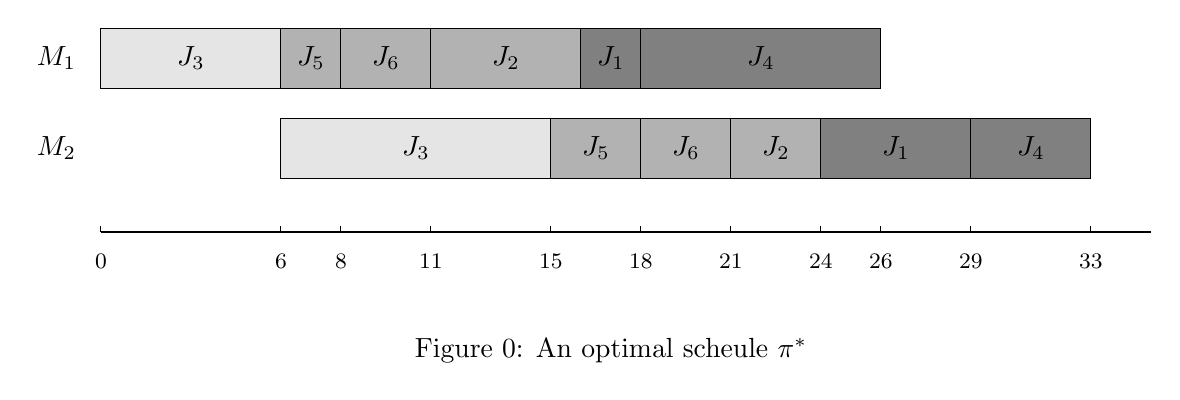
\begin{tikzpicture}[x=0.15in, y=0.3in]
                % machine index
                \node[anchor=east] at (-0.5,5.5) {$M_1$};
                \node[anchor=east] at (-0.5,4) {$M_2$};
                
                % block 1: weight 5 (J_3)
                \draw[fill=gray!20] (0,5)   rectangle (6,6)   node[midway] {$J_3$};
                % block 2: weight 3 (J_5, J_6, J_2)
                \draw[fill=gray!60] (6,5)   rectangle (8,6)   node[midway] {$J_5$};
                \draw[fill=gray!60] (8,5)   rectangle (11,6)  node[midway] {$J_6$};
                \draw[fill=gray!60] (11,5)  rectangle (16,6)  node[midway] {$J_2$};
                % block 3: weight 2 (J_1, J_4)
                \draw[fill=gray!100] (16,5)  rectangle (18,6)  node[midway] {$J_1$};
                \draw[fill=gray!100] (18,5)  rectangle (26,6)  node[midway] {$J_4$};
                
                % block 1
                \draw[fill=gray!20] (6,3.5)  rectangle (15,4.5)  node[midway] {$J_3$};
                % block 2
                \draw[fill=gray!60] (15,3.5)  rectangle (18,4.5)  node[midway] {$J_5$};
                \draw[fill=gray!60] (18,3.5)  rectangle (21,4.5)  node[midway] {$J_6$};
                \draw[fill=gray!60] (21,3.5)  rectangle (24,4.5)  node[midway] {$J_2$};
                % block 3
                \draw[fill=gray!100] (24,3.5)  rectangle (29,4.5)  node[midway] {$J_1$};
                \draw[fill=gray!100] (29,3.5)  rectangle (33,4.5)  node[midway] {$J_4$};
                
                % x-axis
                \draw[thick] (0,2.6) -- (35,2.6);
                \foreach \x/\label in {0/0, 6/6, 8/8, 11/11, 15/15, 18/18, 21/21, 24/24, 26/26, 29/29, 33/33} {
                    \draw (\x,2.6) -- (\x,2.7);
                    \node[below, font=\footnotesize] at (\x,2.4) {\label};
                }
                
                % caption
                \node[below] at (17,1) {Figure~\thefigure: An optimal scheule $\pi^*$};  \label{fig:exam-3};
            \end{tikzpicture}
        \end{figure}
        
        \subsection{An FPTAS for fixed number of weights} \label{sec:fptas}
        
        Let $0 < \epsilon \leq 1$ be real, and let $\delta=1+\epsilon/(2n)$.
        Define the function $\Delta(\cdot)$ on $[0, +\infty)$ by
        \begin{equation} \label{eq-function}
            \Delta(z)=\lfloor \log_{\delta} z \rfloor ~~ (z \geq 1), ~~~~~ \Delta(0)=-1.
        \end{equation}
        Equivalently, if $k$ is an integer that satisfies $\delta^k \leq z < \delta^{k+1}$, then $\Delta(z)=k$.
        
        For fixed $K$, we apply the geometric rounding technique to transform \Cref{alg:dp} into an FPTAS (which we call \Cref{alg-FPTAS}).
        In contrast to \Cref{alg:dp}, the proposed algorithm may remove some non-dominated states in the tuple set generation procedure.
        Let $\mathcal{H}_j^{\epsilon}$ be the set of tuples generated by \Cref{alg-FPTAS} in the $j$-th iteration.
        For each tuple $(X_1, X_2, \ldots, X_K) \in \mathcal{H}_j^{\epsilon}$, define its label to be $(Y_1, Y_2, \ldots, Y_K)$, where $X_k=(A_k, B_k, C_k, L_k)$ for $k=1, 2, \ldots, K$; the first $K-1$ labels are
        \begin{equation*}
            Y_k=(\Delta(A_k), \Delta(B_k), \Delta(C_k), L_k), ~~ 1 \leq k \leq K-1,
        \end{equation*}
        while the last label is
        \begin{equation*}
            Y_K=(\Delta(A_K), \Delta(B_K), L_K).
        \end{equation*}
        By construction, for each $1 \leq k \leq K$ with $A_k \geq 1$, the rounded value $\delta^{\Delta(A_k)}$ approximates $A_k$ up to a small multiplicative error; likewise, $\delta^{\Delta(B_k)}$ and $\delta^{\Delta(C_k)}$ approximate $B_k$ and $C_k$, respectively.
        Hence, whenever two tuples share a label, one of them is eliminated during tuple elimination procedure.
        A formal description of \Cref{alg-FPTAS} is given below.
        
        \begin{algorithm}[H]
            \small
            \linespread{1.2}\selectfont
            \SetAlgoLined
            \DontPrintSemicolon
            \caption{An FPTAS for $F2 \mid \mid C_{\max}^w$}  \label{alg-FPTAS}
            \KwIn{Job set $\mathcal{J}$; error parameter $\epsilon$; job parameters $a_j$, $b_j$, $w_j$, and $g_j$ for $j=1, 2, \ldots, n$; $K$ distinct weights with $W_1> W_2 > \cdots > W_K$.}
            \BlankLine
            \textbf{Step 1.} [Preprocessing] Renumber jobs in $\mathcal{J}$ according to Johnson' rule (\Cref{alg:Johnson}). \;
            
            \textbf{Step 2.} [Initialization] Set $\delta=1+\epsilon/(2n)$. Let  $S_0=\Big(\underbrace{(0,0,0,0),\ldots,(0,0,0,0)}_{K\text{ copies}}\Big)$, and let $R_0=\Big(\underbrace{(-1, -1, -1, 0),\ldots,(-1, -1, -1, 0)}_{K-1\text{ copies}}, (-1, -1, 0)\Big)$ be its label. Initialize $\mathcal{H}_0^{\epsilon}=\{S_0\}$ and $\mathcal{H}_j^{\epsilon}=\emptyset$ for $j=1, 2, \ldots, n$. \;
            
            \textbf{Step 3.} [Generation of sets $\mathcal{H}_1^{\epsilon}, \mathcal{H}_2^{\epsilon}, \ldots, \mathcal{H}_n^{\epsilon}$]
            
            \For{$j=1$ \KwTo $n$}
            {
                \For{each $(X_1, X_2, \ldots, X_K) \in \mathcal{H}_{j-1}^{\epsilon}$ with $X_k=(A_k, B_k, C_k, L_k)$, $k=1, 2, \ldots, K$}
                {
                    \For{$k=1$ \KwTo $g_j$}
                    {
                        $A'_k = A_k+a_j$, $B'_k = B_k+b_j$, $C'_k = \max\{C_{k-1}, A_{k-1}+a_j\}+b_j$, $L'_k= w_j$. \;
                        
                        $X'_k=(A'_k, B'_k, C'_k, L'_k)$. \;
                        
                        \eIf{$k \leq K-1$}
                        {
                            $Y'_k=(\Delta(A'_k), \Delta(B'_k), \Delta(C'_k), L'_k)$. \;
                        }
                        {
                            $Y'_K=(\Delta(A'_K), \Delta(B'_K), L'_K)$. \;
                        }
                        
                        Add the tuple $(X_1, \ldots, X_{k-1}, X'_k, X_{k+1}, \ldots, X_K)$ to $\mathcal{H}_j^{\epsilon}$ and attach the associated label $(Y_1, \ldots, Y_{k-1}, Y'_k, Y_{k+1}, \ldots, Y_K)$ to it. \;
                    }
                }
                [Elimination] Among tuples in $\mathcal{H}_j^{\epsilon}$ sharing identical labels, retain only the one with the smallest $C_K$. \;
            }
            
            \textbf{Step 4.} [Computation of objective values for the tuples in $\mathcal{H}_n^{\epsilon}$]
            
            \For{each $X=(X_1, X_2, \ldots, X_K) \in \mathcal{H}_n^{\epsilon}$ with $X_k=(A_k, B_k, C_k, L_k)$, $k=1, 2, \ldots, K$}
            {
                Perform the same operations as in Step 4 of \Cref{alg:dp}.
            }
            
            \textbf{Step 5.} [Result] Compute $C_{\max}^w(X')=\min \{C_{\max}^w(X): X \in \mathcal{H}_n^{\epsilon}\}$ and recover the corresponding approximate schedule $\pi'$ from $X'$ by backtracking. \;
            
            \KwOut{The approximate schedule $\pi'$.}
        \end{algorithm}
        
        In \Cref{alg-FPTAS}, the box-elimination operation considers coordinate values that increase geometrically.
        Multiplicative errors can occur if, during tuple elimination, each label is represented by the smallest $C_X$ coordinates inside its box rather than by its exact value.
        Nevertheless, the lemma below demonstrates that the tuples left after elimination form a good approximation to those produced by \Cref{alg:dp}.
        
        \begin{lemma}\label{lem:approx}
            Given any tuple $(X_1, X_2, \ldots, X_K) \in \mathcal{H}_j$ generated by \Cref{alg:dp}, where $X_k=(A_k, B_k, C_k, L_k)$ for $k=1, 2, \ldots, K$, \Cref{alg-FPTAS} returns a tuple $(\widetilde{X_1}, \widetilde{X_2}, \ldots, \widetilde{X_K}) \in \mathcal{H}_j^{\epsilon}$, with $\widetilde{X_k}=(\widetilde{A_k}, \widetilde{B_k}, \widetilde{C_k}, L_k)$, such that
            \begin{equation} \label{Eq-conditions}
                \widetilde{A_k} \leq \delta^j A_k, ~~ \widetilde{B_k} \leq \delta^j B_k, ~~ \widetilde{C_k} \leq \delta^j C_k, ~~ k=1, 2, \ldots, K.
            \end{equation}
        \end{lemma}
        
        \begin{proof}
            We prove the result by induction on $j=1, 2, \ldots, n$.
            For the base case $j=1$, $J_1$ can be assigned to each of the $g_1$ schedules (each induced by a block) in \Cref{alg:dp} and \Cref{alg-FPTAS}.
            Since these $g_1$ tuples receive distinct labels in \Cref{alg-FPTAS}, it follows that $\mathcal{H}_1^{\epsilon}=\mathcal{H}_1$, so \cref{Eq-conditions} holds for $j=1$.
            
            Assume that \cref{Eq-conditions} holds for $j-1$ (the induction hypothesis), where $j \geq 2$.
            Let $(X_1, X_2, \ldots, X_K) \in \mathcal{H}_j$ be a tuple obtained from \Cref{alg:dp} for the first $j$ jobs, where $X_k=(A_k, B_k, C_k, L_k)$ for $k=1, 2, \ldots, K$.
            When implementing \Cref{alg:dp}, the tuple $(X_1, X_2, \ldots, X_K)$ is constructed from a tuple $(X'_1, X'_2, \ldots, X'_K) \in \mathcal{H}_{j-1}$, where $X'_k=(A'_k, B'_k, C'_k, L'_k)$ for $k=1, 2, \ldots, K$.
            Specifically, $J_j$ is assigned to one of the $g_j$ schedules corresponding to $(X'_1, X'_2, \ldots, X'_K)$ for the first $j-1$ jobs.
            Based on the induction hypothesis, there exists a tuple $(\widetilde{X'_1}, \widetilde{X'_2}, \ldots, \widetilde{X'_K}) \in \mathcal{H}_{j-1}^{\epsilon}$, where $\widetilde{X'_k}=(\widetilde{A'_k}, \widetilde{B'_k}, \widetilde{C'_k}, L'_k)$, such that
            \begin{equation} \label{Eq-prev}
                \widetilde{A'_k}  \leq \delta^{j-1} A'_k, ~~ \widetilde{B'_k} \leq \delta^{j-1} B'_k, ~~ \widetilde{C'_k} \leq \delta^{j-1} C'_k, ~~ k=1, 2, \ldots, K.
            \end{equation}
            To prove that \cref{Eq-conditions} holds for $j$, consider the $g_j$ possible cases in which $J_j$ is assigned to one of these schedules.
            
            Let $J_j$ be assigned to the $h$-th schedule in \Cref{alg:dp} for some $h \in \{1, 2, \ldots, g_j\}$.
            Then
            \begin{equation} \label{Eq-rec-1}
                \begin{aligned}
                    A_k & =A'_k, ~~ B_k=B'_k ~~, C_k=C'_k ~~, L_k=L'_k, ~~ k \in \{1, 2, \ldots, K\} \setminus \{h\}; \\
                    A_h & =A'_h+a_j, ~~ B_h=B'_h+b_j, ~~ C_h=\max \{C'_h, A'_h+a_j\}+b_j, ~~ L_h=w_j.
                \end{aligned}
            \end{equation}
            Since $(\widetilde{X'_1}, \widetilde{X'_2}, \ldots, \widetilde{X'_K}) \in \mathcal{H}_{j-1}^{\epsilon}$, the tuple $(\widetilde{X'_1}, \widetilde{X'_2}, \ldots, \widetilde{X'_{h-1}}, \overline{X'_h}, \widetilde{X'_{h+1}}, \ldots, \widetilde{X'_K})$ is added to $\mathcal{H}_j^{\epsilon}$ in \Cref{alg-FPTAS}, where $\overline{X'_h}=(\overline{A'_h}, \overline{B'_h}, \overline{C'_h}, \overline{L'_h})$ is defined by
            \begin{equation} \label{Eq-rec-2}
                \overline{A'_h}=\widetilde{A'_h}+a_j, ~~ \overline{B'_h}=\widetilde{B'_h}+b_j, ~~ \overline{C'_h}=\max \{\widetilde{C'_h}, \widetilde{A'_h}+a_j\}+b_j, ~~ \overline{L'_h}=w_j.
            \end{equation}
            Because two tuples can share a label, $(\widetilde{X'_1}, \widetilde{X'_2}, \ldots, \widetilde{X'_{h-1}}, \overline{X'_h}, \widetilde{X'_{h+1}}, \ldots, \widetilde{X'_K})$ may be discarded in \Cref{alg-FPTAS} in favor of another tuple $(\widetilde{X_1}, \widetilde{X_2}, \ldots, \widetilde{X_K}) \in \mathcal{H}_j^{\epsilon}$, where $\widetilde{X_k}=(\widetilde{A_k}, \widetilde{B_k}, \widetilde{C_k}, \widetilde{L_k})$ for $k=1, 2, \ldots, K$.
            For this tuple, by \eqref{Eq-prev}--\eqref{Eq-rec-2} and the construction in \Cref{alg-FPTAS}, we have
            \begin{equation} \label{Eq-fin-1}
                \left \{
                \begin{aligned}
                    \widetilde{A_k} &\leq \delta \widetilde{A'_k} \leq \delta^j A'_k = \delta^j A_k \\
                    \widetilde{B_k} &\leq \delta \widetilde{B'_k} \leq \delta^j B'_k = \delta^j B_k \\
                    \widetilde{L_k} &= \overline{L'_k} = L'_k = L_k
                \end{aligned}
                \right. \qquad \qquad \text{if} ~~ k \in \{1, 2, \ldots, K\}\setminus\{h\};
            \end{equation}
            \begin{equation} \label{Eq-fin-2}
                \left \{
                \begin{aligned}
                    \widetilde{A_h} &\leq \delta \overline{A'_h} = \delta(\widetilde{A'_h}+a_j) \leq \delta(\delta^{j-1}A'_h+a_j)
                    \leq \delta^j(A'_h+a_j) = \delta^j A_h \\
                    \widetilde{B_h} &\leq \delta \overline{B'_h} = \delta(\widetilde{B'_h}+b_j) \leq \delta(\delta^{j-1}B'_h+b_j)
                    \leq \delta^j(B'_h+b_j) = \delta^j B_h \\
                    \widetilde{L_h} &= \overline{L'_h}=w_j=L_h
                \end{aligned}
                \right. ;
            \end{equation}
            \begin{equation} \label{Eq-fin-3}
                \left \{
                \begin{aligned}
                    \widetilde{C_k} & \leq \delta \widetilde{C'_k} \leq \delta^j C'_k = \delta^j C_k && \text{if} ~~ k \in \{1, 2, \ldots, K-1\}\setminus \{h\}\\
                    \widetilde{C_K} & \leq \widetilde{C'_K} \leq \delta^{j-1} C'_K \leq \delta^j C_K  &&  \text{if} ~~ K \neq h
                \end{aligned}
                \right. ;
            \end{equation}
            \begin{equation} \label{Eq-fin-4}
                \left \{
                \begin{aligned}
                    \widetilde{C_h} & \leq \delta \overline{C'_h} = \delta (\max \{\widetilde{C'_h}, \widetilde{A'_h}+a_j\}+b_j) \\
                    & \leq \delta (\max \{\delta^{j-1}C'_h, \delta^{j-1}A'_h+a_j\}+b_j) && \text{if}~~ h \neq K\\
                    & \leq \delta^j (\max\{C'_h, A'_h+a_j\}+b_j) = \delta^j C_h \\
                    \widetilde{C_K} & \leq \overline{C'_K} = \max \{\widetilde{C'_K} \widetilde{A'_K}+a_j\}+b_j \\
                    & \leq  \max \{\delta^{j-1}C'_K, \delta^{j-1}A'_K+a_j\}+b_j && \text{if} ~~ h = K    \\
                    & \leq \delta^{j-1} (\max\{C'_K, A'_K+a_j\}+b_j) \leq \delta^j C_K
                \end{aligned}
                \right. .
            \end{equation}
            
            By \cref{Eq-fin-1}-\cref{Eq-fin-4}, \cref{Eq-conditions} holds for $j$ when $J_j$ is assigned to the $h$-th schedule.
            Since $h$ is arbitrary, this covers every possible assignment of $J_j$.
            Thus, the induction step is established for $j$.
        \end{proof}
        
        To analyze the approximation error and time complexity of \Cref{alg-FPTAS}, we use the following two well-known inequalities.
        The first follows because $f(x)=x \ln x-(x-1)$ is increasing on $[1, +\infty)$ and $f(1)=0$.
        The second follows because $g(x)=(1+\frac{x}{n})^n-(1+2x)$ is convex on $[0, 1]$, with $g(0)=0$ and $g(1) \leq 0$.
        
        \begin{lemma} \label{Lem-ineq-1}
            For any real $x \geq 1$, $\ln x \geq (x-1)/x$.
        \end{lemma}
        
        \begin{lemma} \label{Lem-ineq-2}
            For any real $0 < x \leq 1$, $(1+x/n)^n \leq 1+2x$.
        \end{lemma}
        
        \begin{theorem} \label{Thm-FPTAS}
            For fixed $K$, \Cref{alg-FPTAS} is an FPTAS for $F2 \mid \mid C_{\max}^w$ with $O((n^{3K}/\epsilon^{3K-1}) (\log P)^{3K-1})$ running time.
        \end{theorem}
        
        \begin{proof}
            We first bound the approximation error of the algorithm.
            Let $\pi'$ be the approximate schedule returned by \cref{alg-FPTAS}, and let $\pi_{\mathrm{opt}}$ be the optimal schedule returned by \Cref{alg:dp}.
            Denote by $(X_1^*, X_2^*, \ldots, X_K^*) \in \mathcal{H}_n$ the tuple corresponding to $\pi_{\mathrm{opt}}$, where $X_k^*=(A_k^*, B_k^*, C_k^*, L_k^*)$ for $k=1, 2, \ldots, K$.
            By \cref{eq-4.2:block-makespan} and \cref{eq-4.2:block-weighted makespan}, we have
            \begin{equation} \label{Lem-4.3-fptas-1}
                C_{\max}^w(\pi_{\mathrm{opt}}) =\max_{1 \leq k \leq K} \Big\{W_k \max_{0 \leq h \leq k-1} \Big(\sum_{i=1}^h A_i^* +C_{h+1}^* + \sum_{i=h+2}^k B_i^* \Big)\Big\}.
            \end{equation}
            
            By \Cref{lem:approx}, there exists a tuple $(\widetilde{X_1^*}, \widetilde{X_2^*}, \ldots, \widetilde{X_K^*}) \in \mathcal{H}_n^{\epsilon}$ generated by \Cref{alg-FPTAS}, with $\widetilde{X_k^*}=(\widetilde{A_k^*}, \widetilde{B_k^*}, \widetilde{C_k^*}, L_k^*)$, such that
            \begin{equation} \label{Lem-4.3-fptas-2}
                \widetilde{A_k^*} \leq \delta^n A_k^*, ~~ \widetilde{B_k^*} \leq \delta^n B_k^*, ~~ \widetilde{C_k^*} \leq \delta^n C_k^*, ~~  k=1, 2, \ldots, K.
            \end{equation}
            Let $\widetilde{\pi_{\mathrm{opt}}}$ be the schedule corresponding to $(\widetilde{X_1^*}, \widetilde{X_2^*}, \ldots, \widetilde{X_K^*})$.
            Again by \cref{eq-4.2:block-makespan} and \cref{eq-4.2:block-weighted makespan}, we have
            \begin{equation} \label{Lem-4.3-fptas-3}
                C_{\max}^w(\widetilde{\pi_{\mathrm{opt}}}) =\max_{1 \leq k \leq K} \Big\{W_k \max_{0 \leq h \leq k-1} \Big(\sum_{i=1}^h \widetilde{A_i^*} +\widetilde{C_{h+1}^*} + \sum_{i=h+2}^k \widetilde{B_i^*} \Big)\Big\}.
            \end{equation}
            Recall that $0 < \epsilon \leq 1$ and $\delta=1+\epsilon/(2n)$.
            Then by \Cref{Lem-ineq-2} and \cref{Lem-4.3-fptas-1}--\cref{Lem-4.3-fptas-3}, we have
            \begin{equation*}
                \begin{aligned}
                    C_{\max}^w(\widetilde{\pi_{\mathrm{opt}}}) & \leq \max_{1 \leq k \leq K} \Big\{W_k \max_{0 \leq h \leq k-1} \Big(\sum_{i=1}^h \delta^n A_i^* +\delta^n C_{h+1}^* + \sum_{i=h+2}^k \delta^n B_i^* \Big)\Big\} \\
                    & = \delta^n \max_{1 \leq k \leq K} \Big\{W_k \max_{0 \leq h \leq k-1} \Big(\sum_{i=1}^h  A_i^* + C_{h+1}^* + \sum_{i=h+2}^k B_i^* \Big)\Big\} \\
                    & \leq (1+\epsilon)C_{\max}^w(\pi_{\mathrm{opt}}).
                \end{aligned}
            \end{equation*}
            Thus, from the execution of \Cref{alg-FPTAS}, it returns an approximate schedule $\pi'$ with $C_{\max}^w(\pi') \leq C_{\max}^w(\widetilde{\pi_{\mathrm{opt}}}) \leq (1+\epsilon)C_{\max}^w(\pi_{\mathrm{opt}})$.
            
            We next bound the time complexity of the algorithm.
            Step 1 sorts in $O(n\log n)$ time, and Step 2 initializes in $O(n)$ time.
            In Step 3, at most one tuple is retained per label after elimination.
            For each $(X_1, X_2, \ldots, X_K) \in \mathcal{H}_j^{\epsilon}$ ($j=1, 2, \ldots, n$), the corresponding label is  $(Y_1, Y_2, \ldots, Y_K)$, where $X_k=(A_k, B_k, C_k, L_k)$ for $k=1, 2, \ldots, K$, $Y_k=(\Delta(A_k), \Delta(B_k), \Delta(C_k), L_k)$ for $1 \leq k \leq K-1$, and $Y_K=(\Delta(A_K), \Delta(B_K), L_K)$.
            Note that $A_k \leq P$, $B_k \leq P$, $C_k \leq 2P$, and $L_k \in \{0, W_k, W_{k+1}, \ldots, W_K\}$ for $k=1, 2, \ldots, K$.
            By \Cref{Lem-ineq-1}, the number of distinct values attained by $\Delta(A_k)$ is upper bounded by $1+\lfloor \log_{\delta} P \rfloor = 1+ \lfloor \ln P / \ln \delta \rfloor \leq 1+ \lfloor (1+2n/ \epsilon) \ln P \rfloor =O((n/ \epsilon) \log P)$.
            Analogously, the number of distinct values attained by $\Delta(B_k)$ and $\Delta(C_k)$ are also upper bounded by $O((n/\epsilon) \log P)$.
            Because each tuple yields at most $K$ new tuples, after elimination, the number of retained tuples in $\mathcal{H}_j^{\epsilon}$ is upper bounded by $O((n^{3K-1}/\epsilon^{3K-1}) (\log P)^{3K-1})$.
            Summing the cost of Step 3 over its $n$ iterations gives $O((n^{3K}/\epsilon^{3K-1}) \log P)$ time.
            Step 4 computes the objective value of each tuple in $\mathcal{H}_n^{\epsilon}$ in $O(K)$ time, and thus requires $O((n^{3K-1}/\epsilon^{3K-1}) (\log P)^{3K-1})$ time in total.
            Step 5 has the same time complexity.
            Consequently, the algorithm runs in $O((n^{3K}/\epsilon^{3K-1}) (\log P)^{3K-1})$ time.
        \end{proof}
        
        \subsection{The bounded max-to-min weight ratio} \label{sec:bounded_weight}
        
        Consider the bounded max-to-min ratio weight case where $w_{\max}/w_{\min} \leq C$ for some constant $C$.
        Here, $w_{\max}=\max_{1 \leq j \leq n} \{w_j\}$ is the maximum weight of the $n$ jobs, and $w_{\min}=\min_{1 \leq j \leq n} \{w_j\}$ is the minimum weight.
        The proof of \Cref{thm:nphard} demonstrates that the problem remains $\mathcal{NP}$-hard even when $C=2$.
        
        Let $0 < \epsilon \leq 1$ be a real number.
        For $j=1, 2, \ldots, n$, we round each weight $w_j$ down to the nearest value of the form  $w_{\min}(1+\epsilon/2)^k$, i.e., $\overline{w_j}=w_{\min}(1+\epsilon/2)^{\theta_j}$, where $\theta_j$ is the unique integer satisfying
        \begin{equation} \label{eq-4.4-PTAS-1}
            w_{\min}(1+\epsilon/2)^{\theta_j} \leq w_j < w_{\min}(1+\epsilon/2)^{\theta_j+1}.
        \end{equation}
        
        
        By combining job-weight rounding with the FPTAS in \Cref{sec:fptas}, a PTAS for the bounded max-to-min ratio weight case is given as follows.
        
        \begin{algorithm}[H]
            \small
            \linespread{1.2}\selectfont
            \SetAlgoLined
            \DontPrintSemicolon
            \caption{A PTAS for $F2 \mid \mid C_{\max}^w$ with bounded max-to-min weight ratio}  \label{Alg-PTAS}
            \KwIn{Job set $\mathcal{J}$; error parameter $\epsilon$; job parameters $a_j$, $b_j$, and $w_j$ for $j=1, 2, \ldots, n$.}
            \BlankLine
            \textbf{Step 1.} Construct the rounded instance $\mathcal{I}'$ from the original instance $\mathcal{I}$: replace each job $J_j$ by $J'_j$ with $w'_j=w_{\min}(1+\epsilon/2)^{\theta_j}$, where $\theta_j$ is the integer given by \cref{eq-4.4-PTAS-1}; keep all other job parameters unchanged. \;
            
            \textbf{Step 2.} Let $W_1 >W_2> \cdots >W_K$ be the ordered sequence of distinct rounded weights in $\mathcal{I}'$. Run \Cref{alg-FPTAS} on $\mathcal{I}'$ to obtain a $(1+\epsilon/3)$-approximation schedule $\pi_{\epsilon}$. \;
            
            \KwOut{The approximate schedule $\pi_{\epsilon}$.}
        \end{algorithm}
        
        For a schedule $\pi$, let $C_{\max}^w(\pi, \mathcal{I})=\max_{1 \leq j \leq n}\{ w_{\pi(j)} C_{\pi(j)}(\pi,\mathcal{I})\}$ and $C_{\max}^w(\pi,\mathcal{I}')=\max_{1 \leq j \leq n}\{ w'_{\pi(j)} C_{\pi(j)}(\pi, \mathcal{I}')\}$ denote its weighted makespan on instances $\mathcal{I}$ and $\overline{\mathcal{I}}$, respectively.
        Here, $C_{\pi(j)}(\pi,\mathcal{I})$ and $C_{\pi(j)}(\pi, \mathcal{I}')$ are the completion times of $J_{\pi(j)}$ under $\pi$ on $\mathcal{I}$ and $\mathcal{I}'$, respectively.
        
        \begin{theorem} \label{Theorem-PTAS}
            When $w_{\max}/w_{\min} \leq C$, \Cref{Alg-PTAS} is a PTAS for $F2 \mid \mid C_{\max}^w$ with $O((n^{O(1/\epsilon)}/\epsilon^{O(1/\epsilon)}) (\log P)^{O(1/\epsilon)})$ running time.
        \end{theorem}
        
        \begin{proof}
            Let $\pi_{\mathrm{opt}}$ be an optimal schedule for $\mathcal{I}$, and let $\pi'_{\mathrm{opt}}$ be an optimal schedule for $\mathcal{I}'$.
            Because $\mathcal{I}$ and $\mathcal{I}'$ differ only in their job weights, a fixed schedule $\pi$ yields the same job completion times on both instances, i.e., $C_{\pi(j)}(\pi,\mathcal{I})=C_{\pi(j)}(\pi, \mathcal{I}')$.
            Thus, from the fact that $w'_j \leq w_j < (1+\epsilon/2) w'_j$, $j=1, 2, \ldots, n$, we have
            \begin{equation} \label{Eq-4.4-PTAS-1}
                C_{\max}^w(\pi_{\epsilon}, \mathcal{I}) < (1+\epsilon/2)C_{\max}^w(\pi_{\epsilon}, \mathcal{I}')
            \end{equation}
            and
            \begin{equation} \label{Eq-4.4-PTAS-2}
                C_{\max}^w(\pi'_{\mathrm{opt}}, \mathcal{I}') \leq C_{\max}^w(\pi_{\mathrm{opt}}, \mathcal{I}') \leq C_{\max}^w(\pi_{\mathrm{opt}}, \mathcal{I}).
            \end{equation}
            Since $\pi_{\epsilon}$ is a $(1+\epsilon/3)$-approximation schedule for $\mathcal{I}'$, we have
            \begin{equation} \label{Eq-4.4-PTAS-3}
                C_{\max}^w(\pi_{\epsilon}, \mathcal{I}') \leq (1+\epsilon/3) C_{\max}^w(\pi'_{\mathrm{opt}}, \mathcal{I}').
            \end{equation}
            Then, \cref{Eq-4.4-PTAS-1}--\cref{Eq-4.4-PTAS-3} imply that
            \begin{equation*}
                C_{\max}^w(\pi_{\epsilon}, \mathcal{I}) \leq (1+\epsilon/2) (1+\epsilon/3) C_{\max}^w(\pi'_{\mathrm{opt}}, \mathcal{I}')  \leq  (1+\epsilon)C_{\max}^w(\pi_{\mathrm{opt}},\mathcal{I}).
            \end{equation*}
            
            Let $\mathcal{W}=\{\overline{w_j}: 1 \leq j \leq n\}$ be the set of distinct rounded job weights in $\mathcal{I}'$, and let $K=|\mathcal{W}|$.
            Since $w_{\max}/w_{\min} \leq C$ and $C$ is a constant, we have $K \leq 1+ \lfloor \log_{1+\epsilon/2} C \rfloor =O(1/\epsilon)$.
            The running time is dominated by Step 2.
            By \Cref{Thm-FPTAS}, it requires $O((n^{3K}/\epsilon^{3K-1}) (\log P)^{3K-1})=O((n^{O(1/\epsilon)}/\epsilon^{O(1/\epsilon)}) (\log P)^{O(1/\epsilon)})$ time.
            Consequently, the overall running time is $O((n^{O(1/\epsilon)}/\epsilon^{O(1/\epsilon)}) (\log P)^{O(1/\epsilon)})$.
        \end{proof}
        
        
        
        \section{Heuristic and metaheuristic algorithms} \label{sec:heuristics}
        
        In this section, we first present two constructive heuristics: the largest-weight-first (LW) greedy algorithm, whose worst-case approximation ratio is proved to be 2, and an adapted NEH heuristic that builds a schedule by inserting jobs sequentially. We then develop a genetic algorithm (GA), a metaheuristic that searches over job permutations.
        
        
        \subsection{The LW algorithm} \label{sec:lw}
        
        \cite{Sun2024JOCO} proved that the LW-based greedy algorithm is a $(2-1/m)$-approximation for $Pm \mid \mid C_{\max}^w$. For $F2 \mid \mid C_{\max}^w$, we describe the analogous LW-based algorithm and show that its worst-case approximation ratio is $2$.
        
        \begin{algorithm}[H]
            \small
            \linespread{1.2}\selectfont
            \SetAlgoLined
            \DontPrintSemicolon
            \caption{LW's rule for $F2 \mid \mid C_{\max}^w$} \label{Alg-LW}
            \KwIn{Job set $\mathcal{J}$; job parameters $a_j$, $b_j$, and $w_j$ for $j=1, 2, \ldots, n$.}
            \BlankLine
            \textbf{Step 1.} Renumber the jobs in nonincreasing order of their weights (i.e., the LW order), so that $w_1 \geq w_2 \geq \cdots \geq w_n$. \;
            
            \textbf{Step 2.} Process the jobs in this order on $M_1$ and then on $M_2$, yielding the permutation schedule $\pi_{\mathrm{lw}}$. \;
            
            \KwOut{The resulting schedule $\pi_{\mathrm{lw}}$.}
        \end{algorithm}
        
        \begin{theorem}\label{Thm-LW}
            For $F2 \mid \mid C_{\max}^w$, \Cref{Alg-LW} has a worst-case approximation ratio of $2$, which is tight, and runs in $O(n\log n)$ time.
        \end{theorem}
        
        \begin{proof}
            Since $1 \mid \mid C_{\max}^w$ can be solved in $O(n\log n)$ time by the LW rule \citep{NongChengNg2011EJOR}, we have
            \begin{equation}\label{Eq-LB}
                C_{\max}^w(\pi_{\mathrm{opt}}) \geq \mathrm{LB}=\max \Big \{\max_{1 \leq j \leq n} \Big\{w_j \sum_{i=1}^j a_i \Big\}, \max_{1 \leq j \leq n} \Big\{w_j \sum_{i=1}^j b_i\Big\}, \max_{1 \leq j \leq n} \Big\{w_j (a_j+b_j)\Big\} \Big\},
            \end{equation}
            where the first two terms are machine-based lower bounds and the last is a job-based lower bound.   
            
            By construction, \Cref{Alg-LW} yields $\pi_{\mathrm{lw}}(j)=j$ for $j=1, 2, \ldots, n$. Combining \cref{eq:completion} with  \cref{eq:wcmax}, the weighted makespan of $\pi_{lw}$ can be written as 
            \begin{equation}\label{Eq-LW-WC-1}
                C_{\max}^w(\pi_{\mathrm{lw}}) =\max_{1 \leq j \leq n}\Big\{ w_{\pi_{\mathrm{lw}}(j)} C_{\pi_{\mathrm{lw}}(j)}\Big\}=\max_{1 \leq j \leq n} \Big\{w_j \max_{1 \leq i \leq j} \Big (\sum_{h=1}^{i}a_h + \sum_{h=i}^{j}b_h \Big) \Big\}.
            \end{equation}
            
            By \cref{Eq-LB} and \cref{Eq-LW-WC-1}, we have 
            \begin{equation}\label{Eq-LW-WC-2}
                \begin{aligned}
                    C_{\max}^w(\pi_{\mathrm{lw}}) & \leq \max_{1 \leq j \leq n} \Big\{w_j \sum_{h=1}^{j}a_h + w_j \sum_{h=1}^{j}b_h \Big\} \\
                    & \leq \max_{1 \leq j \leq n} \Big\{w_j \sum_{h=1}^{j}a_h \Big\}+\max_{1 \leq j \leq n} \Big\{w_j \sum_{h=1}^{j}b_h \Big\} \\
                    & \leq 2 C_{\max}^w(\pi_{\mathrm{opt}}).
                \end{aligned}
            \end{equation}
            
            To show that the bound is tight, consider an instance with two jobs: $J_1$ has  $a_1=1+\epsilon$, $b_1=\epsilon$, and $w_1= 1+\epsilon$, and $J_2$ has $a_2=\epsilon$, $b_2=1+\epsilon$, and $w_2= 1$, where $\epsilon > 0$ is arbitrarily small. \Cref{Alg-LW} yields the schedule $\pi_{\mathrm{lw}}=(1,2)$ with $C_{\max}^w(\pi_{\mathrm{lw}})=2+\epsilon$, while the optimal schedule is $\pi_{\mathrm{opt}}=(2,1)$ with $C_{\max}^w(\pi_{\mathrm{opt}})=(1+\epsilon)(1+2\epsilon)$. Hence, $C_{\max}^w(\pi_{\mathrm{lw}})/C_{\max}^w(\pi_{\mathrm{opt}}) \to 2$ as $\epsilon \to 0$.
        \end{proof}
        
        \subsection{The NEH algorithm} \label{sec:neh}
        
        The NEH heuristic is a classical insertion-based constructive method for the permutation flow shop scheduling problem. Following \cite{NawazEnscoreHam1983Omega}, jobs are inserted one at a time: at each iteration, the next job is tested in every feasible position of the current partial schedule, and the position yielding the minimum makespan is selected.
        NEH has proven competitive in flow-shop scheduling and remains widely used \citep{ShaoShaoPi2023ESWA, PukaSkalnaIwona2024COR, WangPanSang2024RCIM, WangPanGao2024CIE}. For the $C_{\max}^w$ objective, two observations motivate our adaptation. First, jobs with large $a_j+b_j$ tend to lengthen the schedule and should therefore be placed early to avoid delaying other jobs. Second, earlier positions reduce completion times, and this reduction has a greater impact on the objective for jobs with larger $w_j$. We therefore prioritize jobs by decreasing $a_j+b_j$, breaking ties by decreasing $w_j$, and insert each job into the position that minimizes the objective value. The procedure is detailed in \Cref{Alg-NEH}. At iteration $k$, evaluating all $k$ insertion positions takes $O(k^2)$ time, so the overall running time is $O(n^3)$.
        
        \begin{algorithm}[H]
            \small
            \linespread{1.2}\selectfont
            \SetAlgoLined
            \DontPrintSemicolon
            \caption{NEH heuristic for $F2 \mid \mid C_{\max}^w$}\label{Alg-NEH}
            \KwIn{Job set $\mathcal{J}$; job parameters $a_j$, $b_j$, and $w_j$ for $j=1, 2, \ldots, n$.}
            \BlankLine
            \textbf{Step 1.} [Preprocessing] Renumber the jobs in $\mathcal{J}$ by nonincreasing $a_j+b_j$, and the ties are broken by nonincreasing $w_j$.  \;
            
            \textbf{Step 2.} [Initialization] $\pi \gets (J_{1})$. \;
            
            \textbf{Step 3.} [Insertion] \For{$k=2$ \KwTo $n$}
            {
                $\pi \gets$ insert $J_{k}$ into $\pi$ at a position that minimizes $C_{\max}^w$. \;
            }
            \KwOut{The resulting schedule $\pi$.}
        \end{algorithm}
        
        \subsection{The genetic algorithm} \label{sec:ga}
        
        Genetic algorithms are widely used for scheduling problems, with operators designed around problem-specific structure. Recent flow-shop studies have tailored genetic operators to blocking constraints \citep{deAthaydePrataFuchigami2024JIM}, sequence-independent setup times with non-interruption requirements \citep{QiaoWuHeLi2022ESA}, and energy consumption under variable machine speeds \citep{WangWang2023EAAI}. For the 
        $C_{\max}^w$ objective, \Cref{lem:block-johnson} implies that an optimal schedule is composed of weight-based blocks, with jobs inside each block ordered by Johnson's rule. Building on this structure, we develop a weight-block genetic algorithm (\Cref{Alg-GA}) whose key component is a weight-class-based mutation operator.
        
        Each chromosome encodes a job permutation. The initial population consists of the schedule generated by Johnson's rule and $N-1$ adjacent-swap variants of it, where $N$ is the population size. Although Johnson's rule ignores job weights, it provides a structured, makespan-oriented schedule that serves as a starting point for the weight-aware search. Parents are chosen by fitness-based binary tournament. The offspring then undergo partially mapped crossover and weight-class-based mutation. Elitism retains the $N$ best individuals from the combined parent–offspring pool.
        
        The weight-class mutation operator is a key feature of \Cref{Alg-GA}. Rather than moving individual jobs, it extracts an entire weight class, keeps its internal order, and reinserts the class as a block at the position minimizing $C_{\max}^w$. The class is chosen with equal probability either uniformly at random or from classes containing a job attaining the current $C_{\max}^w$. This block move exploits the problem structure. Since a forward move can delay the jobs it passes, it may not improve the schedule; selection then decides whether it is retained. A local search subsequently relocates the $k$ jobs with the largest $w_j C_j$ values, one at a time, to positions minimizing $C_{\max}^w$. It terminates after $G$ rounds or when a round yields no improvement in $C_{\max}^w$. To balance solution quality against computation time, GA uses population size $N=\min\{20,\max\{6,\lceil n/2\rceil\}\}$. For small instances, the generation count is $G=\max\{1,\lfloor(n-5)/5\rfloor\}$ and the offspring count per generation is $\lambda=\max\{1,\lfloor\max\{0,n-20\}^2/20\rfloor\}$; for large instances, $G=1+\lfloor(n-100)/50\rfloor$ and $\lambda=\max\{3,\lfloor 3n^3/10^6\rfloor\}$. 
        
        \begin{algorithm}[H]
            \small
            \linespread{1.2}\selectfont
            \SetAlgoLined
            \DontPrintSemicolon
            \caption{The weight-block genetic algorithm (WBGA) for $F2 \mid \mid C_{\max}^w$} \label{Alg-GA}
            
            \KwIn{Job set $\mathcal{J}$; number of distinct weights $K$; population size
                $N$; generations $G$; offspring $\lambda$; probabilities $p_c$, $p_m$;
                reinsertion count $k$.}
            \BlankLine
            \textbf{Step 1.} [Initialization] $P_0\gets$ Johnson's schedule and $N-1$ adjacent-swap variants; evaluate. \;
            
            \textbf{Step 2.} [Evolution] \For{$g=1$ \KwTo $G$}
            {
                \textbf{Selection} $M_g\gets$ binary tournament on $P_{g-1}$. \;
                
                \textbf{Crossover} \While{$|O_g|<\lambda$}
                {
                    Draw $\pi_1,\pi_2$ from $M_g$; with probability $p_c$ obtain two children by block crossover, otherwise copy the parents; add them to $O_g$. \;
                }
                
                \textbf{Mutation} Apply block mutation to each child with probability $p_m$; evaluate. \;
                
                \textbf{Survival} $P_g\gets$ the $N$ best of $P_{g-1}\cup O_g$ by $C_{\max}^w$. \;
            }
            
            $\pi^{*}\gets$ the best of $P_G$. \;
            
            \textbf{Step 3.} [Local search] \Repeat{no reinsertion lowers $C_{\max}^w(\pi^{*})$, or $G$ rounds have been reached}
            {
                $J_1,\ldots,J_k\gets$ the $k$ jobs of $\pi^{*}$ with the largest $w_jC_j$. \;
                
                $\pi'\gets$ best schedule from removing one $J_i$ and reinserting it at one position. \;
                
                \If{$C_{\max}^w(\pi')<C_{\max}^w(\pi^{*})$}{$\pi^{*}\gets\pi'$ \;}
            }
            \KwOut{$\pi^{*}$.}
        \end{algorithm}
        
        
        \section{Numerical experiments} \label{sec:experiments}
        
        In this section, we carry out a series of computational experiments to examine the performance of the proposed exact and heuristic methods. All algorithms were implemented in Python 3.13 and tested on a computer running Windows 11, equipped with an Intel Core Ultra 5 230F processor and 16 GB of RAM. The MILP model was solved using Gurobi 13.0 with a single thread.
        
        \subsection{Experimental setup} \label{sec:setup}
        
        To enable a fair and systematic comparison, we divided the experiments into three groups and controlled the parameter settings within each group. Let $\mathrm{UD}[a, b]$ denote the uniform distribution over the consecutive integers $a, a+1, \ldots, b$. For each group, problem instances were generated randomly from the prescribed uniform distributions. Each configuration comprised 20 independently generated instances, and each instance had a time limit of 600 s.
        
        Group 1 concerns only the exact DP algorithm in \Cref{sec:dp} and evaluates its running time in seconds (s), with $p_{\max} \in \{40, 80\}$ and $a_j, b_j \sim UD[1, p_{\max}]$. With two distinct weight values, $w_j \in \{1,10\}$, the instance sizes are $n \in \{20,40,50,60,120,140\}$; with three values, $w_j \in \{1,10,100\}$, they are $n \in \{10,20,30,40\}$. These values only capture differences among jobs and do not affect the running time. 
        
        Groups 2 and 3 evaluate the three heuristic algorithms LW, NEH, and GA in \Cref{sec:heuristics}  using running time in milliseconds (ms) and the relative percentage gap in \Cref{eq:gap}. Group 2 uses small-scale instances ($n \in \{10,15,\ldots,55\}$), and Group 3 use large-scale instances ($n \in \{100,120,\ldots,400\}$), it is computed relative to a prescribed lower bound. In both groups, $a_j, b_j \sim UD[1, p_{\max}]$ and $w_j \sim UD[1, w_{\max}]$, where $p_{\max} \in \{40, 80\}$ and $w_{\max} \in \{30, 100\}$.
        
        The relative percentage gap is
        \begin{equation}\label{eq:gap}
            \text{gap}_A =
            \frac{z_A-z_{\text{base}}}{z_{\text{base}}}\times 100\%,
        \end{equation}
        where $z_A$ is the objective value returned by heuristic $A$, with $A \in\{LW, NEH, GA\}$, and $z_{\text{base}}$ is the reference value. For small-scale instances, $z_{\text{base}}$ is the optimal objective value of the MILP model; for large-scale instances, it is the lower bound LB given in \Cref{Eq-LB}.
        
        \subsection{Computational results} \label{sec:results}
        
        The $DP$ is substantially faster when applicable.
        With 2 weight values, it certifies optimality for all 20 instances at each tested size up to 60 jobs, for 19 and 2 of the 20 instances at 120 jobs under $[1,40]$ and $[1,80]$, respectively, and for 16 of the 20 instances at 140 jobs (\Cref{tab:results-dp-k2}).
        With 3 weight values, however, its running time increases much more rapidly.
        All 20 instances are solved within the time limit at 10 and 20 jobs, with mean running times below 0.01 s at 10 jobs and 1.09 s and 1.59 s at 20 jobs under $[1,40]$ and $[1,80]$, respectively.
        At 30 jobs, the mean running time increases to 58.67 s and 91.51 s, approximately fifty times the corresponding 20-job values, and one instance under $[1,80]$ reaches the 600 s time limit.
        At 40 jobs, all instances exceed the time limit, and none is solved to optimality; accordingly, the corresponding row is left blank in \Cref{tab:results-dp-k3}.

        The $MILP$ model certifies optimality for almost all small instances, although its mean running time increases from $70$ ms at 10 jobs to $110\,000$ ms at 55 jobs (\Crefrange{tab:results-small-40}{tab:results-small100-80}).
        On small instances, the three heuristics differ primarily in solution quality.
        With $w_{\max}=30$, $NEH$ achieves the smallest mean gap in most configurations, ranging from 0.8\% to 5.0\%, compared with 4.5\% to 8.1\% for $LW$.
        $GA$ is the least accurate on small instances, although its mean gap decreases from 12.6\% and 14.3\% at 10 jobs to 4.2\% and 3.5\% at 55 jobs under the two processing-time ranges (\Crefrange{tab:results-small-40}{tab:results-small-80} and \Cref{fig:gap-small}).
        With $w_{\max}=100$, $NEH$ remains the most accurate, with mean gaps ranging from 1.1\% to 5.2\%, while $LW$ ranges from 3.8\% to 9.1\%. 
        In contrast, $GA$ maintains mean gaps between 14.7\% and 26.8\%, with no substantial improvement as the number of jobs increases (\Crefrange{tab:results-small100-40}{tab:results-small100-80} and \Cref{fig:gap-small-k100}).
        In terms of computational cost, $LW$ is the fastest, followed closely by $NEH$, whereas $GA$ is considerably slower, with its mean running time increasing from $0.64$ ms at 10 jobs to $1\,000$ ms at 55 jobs.

        On large instances, the three heuristics differ primarily in how their solution quality is affected by the number of weight values.
        With $w_{\max}=30$, $LW$ achieves the smallest mean gap in most configurations, ranging from 1.4\% to 4.4\%, while the gap of $NEH$ ranges from 3.9\% to 6.0\%. 
        By contrast, $GA$ performs worst at 100 jobs, with mean gaps of 18.3\% and 16.0\% under $[1,40]$ and $[1,80]$, respectively.
        Its mean gap nevertheless decreases to 0.6\% and 0.8\% at 400 jobs, allowing $GA$ to outperform $LW$ in solution quality from 220 jobs under $[1,40]$ and from 240 jobs under $[1,80]$ (\Crefrange{tab:results-large-40}{tab:results-large-80} and \Cref{fig:gap-large}).
        With $w_{\max}=100$, $LW$ remains the most accurate, with mean gaps ranging from 1.6\% to 4.4\%, while those of $NEH$ range from 5.0\% to 7.6\%. 
        In contrast, $GA$ maintains mean gaps between 17.5\% and 50.7\%, and no longer achieves the accuracy advantage observed with 30 weight values (\Crefrange{tab:results-large100-40}{tab:results-large100-80} and \Cref{fig:gap-large-k100}).
        This improvement in solution quality comes at a substantial computational cost: under $[1,40]$, $GA$ requires 128\,000 ms at 400 jobs, compared with 0.146 ms for $LW$ and 2\,180 ms for $NEH$.

        Overall, the $DP$ certifies optimality for all instances with up to 60 jobs and two weight values, but fails to solve all instances at 40 jobs with three weight values.
        Among the heuristics, $LW$ is the fastest and maintains a mean gap below 9.1\% across all configurations, while $NEH$ achieves the smallest mean gaps on most small instances.
        $GA$ is most competitive on large instances with few weight values, where its mean gap decreases from 18.3\% at 100 jobs to 0.6\% at 400 jobs, at the cost of a running time approximately six orders of magnitude longer than that of $LW$.


        \begin{table}[H]
            \resultstable
            \setlength{\tabcolsep}{27.0pt}
            \caption{DP, weights $\in\{1,10\}$}
            \label{tab:results-dp-k2}
            \begin{tabular}{@{}l r r r @{\hspace{14pt}} r r r@{}}
                \toprule
                \multirow{3}{*}{$n$} & \multicolumn{3}{c}{$a_j,b_j\in[1,40]$} & \multicolumn{3}{c}{$a_j,b_j\in[1,80]$} \\
                \cmidrule(lr){2-4}\cmidrule(lr){5-7}
                & \multicolumn{2}{c}{time (s)} & opt. & \multicolumn{2}{c}{time (s)} & opt. \\
                \cmidrule(lr){2-3}\cmidrule(lr){5-6}
                & avg & max & & avg & max & \\
                \midrule
                $20$ & $0.01$ & $0.11$ & $20/20$ & $0.01$ & $0.08$ & $20/20$ \\
                $40$ & $2.41$ & $7.02$ & $20/20$ & $7.95$ & $32.37$ & $20/20$ \\
                $50$ & $11.80$ & $24.25$ & $20/20$ & $28.90$ & $63.55$ & $20/20$ \\
                $60$ & $25.05$ & $58.58$ & $20/20$ & $78.55$ & $176.76$ & $20/20$ \\
                $120$ & $269.83$ & $600.00$ & $19/20$ & $565.30$ & $600.00$ & $2/20$ \\
                $140$ & $405.57$ & $600.00$ & $16/20$ & $--$ & $--$ & $--$ \\
                \bottomrule
            \end{tabular}
            \par\vspace{2pt}
        \end{table}

        \begin{table}[H]
            \resultstable
            \setlength{\tabcolsep}{28.5pt}
            \caption{DP, weights $\in\{1,10,100\}$}
            \label{tab:results-dp-k3}
            \begin{tabular}{@{}l r r r @{\hspace{14pt}} r r r@{}}
                \toprule
                \multirow{3}{*}{$n$} & \multicolumn{3}{c}{$a_j,b_j\in[1,40]$} & \multicolumn{3}{c}{$a_j,b_j\in[1,80]$} \\
                \cmidrule(lr){2-4}\cmidrule(lr){5-7}
                & \multicolumn{2}{c}{time (s)} & opt. & \multicolumn{2}{c}{time (s)} & opt. \\
                \cmidrule(lr){2-3}\cmidrule(lr){5-6}
                & avg & max & & avg & max & \\
                \midrule
                $10$ & $0.00$ & $0.01$ & $20/20$ & $0.00$ & $0.00$ & $20/20$ \\
                $20$ & $1.09$ & $4.21$ & $20/20$ & $1.59$ & $6.56$ & $20/20$ \\
                $30$ & $58.67$ & $417.68$ & $20/20$ & $91.51$ & $600.00$ & $19/20$ \\
                $40$ & $--$ & $--$ & $--$ & $--$ & $--$ & $--$ \\
                \bottomrule
            \end{tabular}
            \par\vspace{2pt}
        \end{table}

        \begin{table}[H]
            \resultstable
            \setlength{\tabcolsep}{4.9pt}
            \caption{Small scale, $p_{\max}=40$, weights $\in\{1,\ldots,30\}$}
            \label{tab:results-small-40}
            \begin{tabular}{@{}l r r @{\hspace{5pt}} r r r r @{\hspace{5pt}} r r r r @{\hspace{5pt}} r r r r@{}}
                \toprule
                \multirow{3}{*}{$n$} & \multicolumn{2}{c}{MILP} & \multicolumn{4}{c}{LW} & \multicolumn{4}{c}{NEH} & \multicolumn{4}{c}{GA} \\
                \cmidrule(lr){2-3}\cmidrule(lr){4-7}\cmidrule(lr){8-11}\cmidrule(lr){12-15}
                & \multicolumn{2}{c}{time (ms)} & \multicolumn{2}{c}{gap} & \multicolumn{2}{c}{time (ms)} & \multicolumn{2}{c}{gap} & \multicolumn{2}{c}{time (ms)} & \multicolumn{2}{c}{gap} & \multicolumn{2}{c}{time (ms)} \\
                \cmidrule(lr){2-3}\cmidrule(lr){4-5}\cmidrule(lr){6-7}\cmidrule(lr){8-9}\cmidrule(lr){10-11}\cmidrule(lr){12-13}\cmidrule(lr){14-15}
                & avg & max & avg & max & avg & max & avg & max & avg & max & avg & max & avg & max \\
                \midrule
                $10$ & $7.0\mathrm{e}1$ & $1.2\mathrm{e}2$ & $7.3$ & $17.2$ & $8.8\mathrm{e}{-3}$ & $2.5\mathrm{e}{-2}$ & $\mathbf{3.4}$ & $24.9$ & $7.3\mathrm{e}{-2}$ & $7.9\mathrm{e}{-2}$ & $12.6$ & $30.6$ & $6.4\mathrm{e}{-1}$ & $7.2\mathrm{e}{-1}$ \\
                $15$ & $1.9\mathrm{e}2$ & $4.7\mathrm{e}2$ & $6.8$ & $16.9$ & $9.9\mathrm{e}{-3}$ & $1.9\mathrm{e}{-2}$ & $\mathbf{2.1}$ & $8.5$ & $1.9\mathrm{e}{-1}$ & $2.0\mathrm{e}{-1}$ & $18.2$ & $49.5$ & $2.6\mathrm{e}0$ & $2.9\mathrm{e}0$ \\
                $20$ & $5.6\mathrm{e}2$ & $1.9\mathrm{e}3$ & $6.2$ & $19.9$ & $1.3\mathrm{e}{-2}$ & $2.3\mathrm{e}{-2}$ & $\mathbf{2.7}$ & $11.7$ & $3.8\mathrm{e}{-1}$ & $4.1\mathrm{e}{-1}$ & $12.1$ & $33.0$ & $1.0\mathrm{e}1$ & $1.1\mathrm{e}1$ \\
                $25$ & $1.5\mathrm{e}3$ & $5.7\mathrm{e}3$ & $5.6$ & $21.5$ & $1.4\mathrm{e}{-2}$ & $2.5\mathrm{e}{-2}$ & $\mathbf{3.7}$ & $17.5$ & $7.0\mathrm{e}{-1}$ & $7.4\mathrm{e}{-1}$ & $15.3$ & $57.5$ & $2.8\mathrm{e}1$ & $3.3\mathrm{e}1$ \\
                $30$ & $2.8\mathrm{e}3$ & $1.0\mathrm{e}4$ & $5.6$ & $14.9$ & $1.4\mathrm{e}{-2}$ & $2.6\mathrm{e}{-2}$ & $\mathbf{3.9}$ & $10.8$ & $1.1\mathrm{e}0$ & $1.2\mathrm{e}0$ & $11.6$ & $26.7$ & $6.2\mathrm{e}1$ & $7.0\mathrm{e}1$ \\
                $35$ & $8.4\mathrm{e}3$ & $3.6\mathrm{e}4$ & $5.7$ & $12.2$ & $1.4\mathrm{e}{-2}$ & $2.4\mathrm{e}{-2}$ & $\mathbf{3.2}$ & $13.8$ & $1.8\mathrm{e}0$ & $1.8\mathrm{e}0$ & $12.8$ & $38.7$ & $1.2\mathrm{e}2$ & $1.3\mathrm{e}2$ \\
                $40$ & $2.1\mathrm{e}4$ & $1.2\mathrm{e}5$ & $4.9$ & $10.6$ & $1.7\mathrm{e}{-2}$ & $3.0\mathrm{e}{-2}$ & $\mathbf{2.4}$ & $6.2$ & $2.5\mathrm{e}0$ & $2.6\mathrm{e}0$ & $7.0$ & $17.5$ & $2.4\mathrm{e}2$ & $2.5\mathrm{e}2$ \\
                $45$ & $3.1\mathrm{e}4$ & $2.5\mathrm{e}5$ & $6.0$ & $19.0$ & $1.8\mathrm{e}{-2}$ & $3.8\mathrm{e}{-2}$ & $\mathbf{3.7}$ & $10.3$ & $3.5\mathrm{e}0$ & $3.7\mathrm{e}0$ & $8.8$ & $24.7$ & $4.1\mathrm{e}2$ & $4.5\mathrm{e}2$ \\
                $50$ & $8.4\mathrm{e}4$ & $5.1\mathrm{e}5$ & $4.5$ & $13.0$ & $1.8\mathrm{e}{-2}$ & $3.1\mathrm{e}{-2}$ & $\mathbf{3.6}$ & $8.4$ & $4.8\mathrm{e}0$ & $4.9\mathrm{e}0$ & $6.5$ & $22.9$ & $6.7\mathrm{e}2$ & $7.3\mathrm{e}2$ \\
                $55$ & $1.1\mathrm{e}5$ & $5.2\mathrm{e}5$ & $4.7$ & $10.9$ & $2.7\mathrm{e}{-2}$ & $4.7\mathrm{e}{-2}$ & $\mathbf{3.1}$ & $11.9$ & $6.2\mathrm{e}0$ & $6.4\mathrm{e}0$ & $4.2$ & $14.6$ & $1.0\mathrm{e}3$ & $1.2\mathrm{e}3$ \\
                \bottomrule
            \end{tabular}
        \end{table}

        \begin{table}[H]
            \resultstable
            \setlength{\tabcolsep}{4.9pt}
            \caption{Small scale, $p_{\max}=80$, weights $\in\{1,\ldots,30\}$}
            \label{tab:results-small-80}
            \begin{tabular}{@{}l r r @{\hspace{5pt}} r r r r @{\hspace{5pt}} r r r r @{\hspace{5pt}} r r r r@{}}
                \toprule
                \multirow{3}{*}{$n$} & \multicolumn{2}{c}{MILP} & \multicolumn{4}{c}{LW} & \multicolumn{4}{c}{NEH} & \multicolumn{4}{c}{GA} \\
                \cmidrule(lr){2-3}\cmidrule(lr){4-7}\cmidrule(lr){8-11}\cmidrule(lr){12-15}
                & \multicolumn{2}{c}{time (ms)} & \multicolumn{2}{c}{gap} & \multicolumn{2}{c}{time (ms)} & \multicolumn{2}{c}{gap} & \multicolumn{2}{c}{time (ms)} & \multicolumn{2}{c}{gap} & \multicolumn{2}{c}{time (ms)} \\
                \cmidrule(lr){2-3}\cmidrule(lr){4-5}\cmidrule(lr){6-7}\cmidrule(lr){8-9}\cmidrule(lr){10-11}\cmidrule(lr){12-13}\cmidrule(lr){14-15}
                & avg & max & avg & max & avg & max & avg & max & avg & max & avg & max & avg & max \\
                \midrule
                $10$ & $5.1\mathrm{e}1$ & $1.0\mathrm{e}2$ & $8.1$ & $17.5$ & $8.5\mathrm{e}{-3}$ & $1.8\mathrm{e}{-2}$ & $\mathbf{0.8}$ & $5.7$ & $7.2\mathrm{e}{-2}$ & $7.8\mathrm{e}{-2}$ & $14.3$ & $47.5$ & $6.1\mathrm{e}{-1}$ & $6.8\mathrm{e}{-1}$ \\
                $15$ & $2.9\mathrm{e}2$ & $1.8\mathrm{e}3$ & $7.7$ & $19.7$ & $9.5\mathrm{e}{-3}$ & $2.0\mathrm{e}{-2}$ & $\mathbf{2.4}$ & $14.5$ & $1.9\mathrm{e}{-1}$ & $2.1\mathrm{e}{-1}$ & $15.9$ & $37.5$ & $2.6\mathrm{e}0$ & $2.9\mathrm{e}0$ \\
                $20$ & $4.5\mathrm{e}2$ & $1.8\mathrm{e}3$ & $4.5$ & $11.8$ & $1.2\mathrm{e}{-2}$ & $2.9\mathrm{e}{-2}$ & $\mathbf{2.6}$ & $9.6$ & $3.8\mathrm{e}{-1}$ & $4.1\mathrm{e}{-1}$ & $16.3$ & $39.1$ & $1.0\mathrm{e}1$ & $1.2\mathrm{e}1$ \\
                $25$ & $1.6\mathrm{e}3$ & $4.6\mathrm{e}3$ & $4.7$ & $16.2$ & $1.2\mathrm{e}{-2}$ & $2.1\mathrm{e}{-2}$ & $\mathbf{2.1}$ & $7.9$ & $7.0\mathrm{e}{-1}$ & $7.4\mathrm{e}{-1}$ & $15.7$ & $37.6$ & $2.8\mathrm{e}1$ & $3.0\mathrm{e}1$ \\
                $30$ & $3.2\mathrm{e}3$ & $9.5\mathrm{e}3$ & $5.6$ & $11.7$ & $1.5\mathrm{e}{-2}$ & $2.9\mathrm{e}{-2}$ & $\mathbf{2.6}$ & $13.6$ & $1.2\mathrm{e}0$ & $1.2\mathrm{e}0$ & $14.4$ & $34.2$ & $6.1\mathrm{e}1$ & $6.6\mathrm{e}1$ \\
                $35$ & $8.7\mathrm{e}3$ & $4.1\mathrm{e}4$ & $7.0$ & $18.1$ & $1.8\mathrm{e}{-2}$ & $3.1\mathrm{e}{-2}$ & $\mathbf{4.3}$ & $7.9$ & $1.8\mathrm{e}0$ & $1.8\mathrm{e}0$ & $11.5$ & $27.5$ & $1.2\mathrm{e}2$ & $1.3\mathrm{e}2$ \\
                $40$ & $2.4\mathrm{e}4$ & $1.5\mathrm{e}5$ & $6.3$ & $20.8$ & $1.8\mathrm{e}{-2}$ & $3.1\mathrm{e}{-2}$ & $\mathbf{2.4}$ & $7.6$ & $2.5\mathrm{e}0$ & $2.6\mathrm{e}0$ & $5.5$ & $15.9$ & $2.5\mathrm{e}2$ & $2.7\mathrm{e}2$ \\
                $45$ & $6.8\mathrm{e}4$ & $3.8\mathrm{e}5$ & $4.8$ & $12.3$ & $1.6\mathrm{e}{-2}$ & $1.9\mathrm{e}{-2}$ & $\mathbf{2.8}$ & $11.9$ & $3.5\mathrm{e}0$ & $3.7\mathrm{e}0$ & $5.3$ & $13.1$ & $4.2\mathrm{e}2$ & $4.5\mathrm{e}2$ \\
                $50$ & $7.7\mathrm{e}4$ & $4.8\mathrm{e}5$ & $6.2$ & $12.4$ & $1.9\mathrm{e}{-2}$ & $3.0\mathrm{e}{-2}$ & $\mathbf{3.8}$ & $11.1$ & $4.7\mathrm{e}0$ & $4.8\mathrm{e}0$ & $4.2$ & $12.0$ & $6.6\mathrm{e}2$ & $7.4\mathrm{e}2$ \\
                $55$ & $1.4\mathrm{e}5$ & $4.7\mathrm{e}5$ & $5.0$ & $11.4$ & $2.2\mathrm{e}{-2}$ & $3.9\mathrm{e}{-2}$ & $5.0$ & $16.2$ & $6.2\mathrm{e}0$ & $6.5\mathrm{e}0$ & $\mathbf{3.5}$ & $14.7$ & $1.1\mathrm{e}3$ & $1.2\mathrm{e}3$ \\
                \bottomrule
            \end{tabular}
        \end{table}

        \begin{figure}[H]
            \centering
            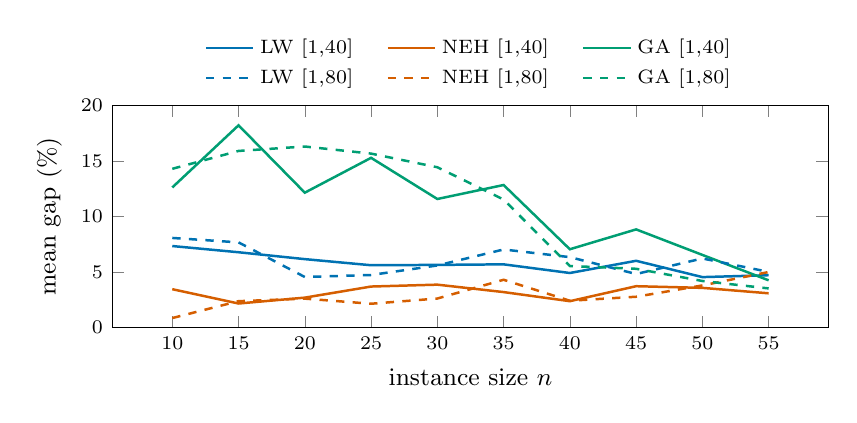
\begin{tikzpicture}
                \begin{axis}[
                    width=0.88\textwidth, height=4.4cm,
                    xlabel={instance size $n$}, ylabel={mean gap (\%)},
                    xtick={10,15,20,25,30,35,40,45,50,55}, xticklabels={10,15,20,25,30,35,40,45,50,55},
                    ymin=0, ymax=20,
                    tick label style={font=\scriptsize}, label style={font=\small},
                    every axis plot/.append style={line width=0.9pt},
                    legend columns=3,
                    legend style={font=\scriptsize, at={(0.5,1.03)}, anchor=south, draw=none,
                        /tikz/every even column/.append style={column sep=10pt}},
                    ]
                    \addplot[apxblue] coordinates {(10,7.33) (15,6.77) (20,6.15) (25,5.60) (30,5.63) (35,5.68) (40,4.90) (45,6.00) (50,4.53) (55,4.70)};
                    \addlegendentry{LW $[1{,}40]$}
                    \addplot[nehred] coordinates {(10,3.44) (15,2.15) (20,2.68) (25,3.68) (30,3.85) (35,3.18) (40,2.36) (45,3.71) (50,3.56) (55,3.07)};
                    \addlegendentry{NEH $[1{,}40]$}
                    \addplot[gagreen] coordinates {(10,12.61) (15,18.21) (20,12.14) (25,15.28) (30,11.57) (35,12.83) (40,7.04) (45,8.83) (50,6.53) (55,4.24)};
                    \addlegendentry{GA $[1{,}40]$}
                    \addplot[apxblue, dashed] coordinates {(10,8.06) (15,7.66) (20,4.54) (25,4.72) (30,5.58) (35,7.02) (40,6.33) (45,4.81) (50,6.21) (55,5.00)};
                    \addlegendentry{LW $[1{,}80]$}
                    \addplot[nehred, dashed] coordinates {(10,0.84) (15,2.36) (20,2.59) (25,2.13) (30,2.60) (35,4.29) (40,2.40) (45,2.76) (50,3.78) (55,4.99)};
                    \addlegendentry{NEH $[1{,}80]$}
                    \addplot[gagreen, dashed] coordinates {(10,14.29) (15,15.90) (20,16.30) (25,15.66) (30,14.43) (35,11.52) (40,5.53) (45,5.28) (50,4.18) (55,3.51)};
                    \addlegendentry{GA $[1{,}80]$}
                \end{axis}
            \end{tikzpicture}
            \caption{Small scale, weights $\in\{1,\ldots,30\}$.}
            \label{fig:gap-small}
        \end{figure}

        \begin{table}[H]
            \resultstable
            \setlength{\tabcolsep}{4.9pt}
            \caption{Small scale, $p_{\max}=40$, weights $\in\{1,\ldots,100\}$}
            \label{tab:results-small100-40}
            \begin{tabular}{@{}l r r @{\hspace{5pt}} r r r r @{\hspace{5pt}} r r r r @{\hspace{5pt}} r r r r@{}}
                \toprule
                \multirow{3}{*}{$n$} & \multicolumn{2}{c}{MILP} & \multicolumn{4}{c}{LW} & \multicolumn{4}{c}{NEH} & \multicolumn{4}{c}{GA} \\
                \cmidrule(lr){2-3}\cmidrule(lr){4-7}\cmidrule(lr){8-11}\cmidrule(lr){12-15}
                & \multicolumn{2}{c}{time (ms)} & \multicolumn{2}{c}{gap} & \multicolumn{2}{c}{time (ms)} & \multicolumn{2}{c}{gap} & \multicolumn{2}{c}{time (ms)} & \multicolumn{2}{c}{gap} & \multicolumn{2}{c}{time (ms)} \\
                \cmidrule(lr){2-3}\cmidrule(lr){4-5}\cmidrule(lr){6-7}\cmidrule(lr){8-9}\cmidrule(lr){10-11}\cmidrule(lr){12-13}\cmidrule(lr){14-15}
                & avg & max & avg & max & avg & max & avg & max & avg & max & avg & max & avg & max \\
                \midrule
                $10$ & $7.0\mathrm{e}1$ & $1.4\mathrm{e}2$ & $6.5$ & $23.9$ & $8.2\mathrm{e}{-3}$ & $1.6\mathrm{e}{-2}$ & $\mathbf{1.1}$ & $9.0$ & $7.4\mathrm{e}{-2}$ & $8.1\mathrm{e}{-2}$ & $20.6$ & $60.4$ & $6.4\mathrm{e}{-1}$ & $7.7\mathrm{e}{-1}$ \\
                $15$ & $2.0\mathrm{e}2$ & $4.4\mathrm{e}2$ & $6.8$ & $29.3$ & $1.0\mathrm{e}{-2}$ & $1.9\mathrm{e}{-2}$ & $\mathbf{2.7}$ & $22.9$ & $1.9\mathrm{e}{-1}$ & $2.2\mathrm{e}{-1}$ & $21.2$ & $51.3$ & $2.6\mathrm{e}0$ & $3.0\mathrm{e}0$ \\
                $20$ & $3.8\mathrm{e}2$ & $6.2\mathrm{e}2$ & $4.7$ & $19.8$ & $1.1\mathrm{e}{-2}$ & $2.4\mathrm{e}{-2}$ & $\mathbf{2.6}$ & $11.0$ & $3.9\mathrm{e}{-1}$ & $4.9\mathrm{e}{-1}$ & $20.1$ & $42.0$ & $1.1\mathrm{e}1$ & $1.2\mathrm{e}1$ \\
                $25$ & $1.3\mathrm{e}3$ & $2.9\mathrm{e}3$ & $6.6$ & $16.7$ & $1.3\mathrm{e}{-2}$ & $2.3\mathrm{e}{-2}$ & $\mathbf{2.4}$ & $9.2$ & $7.1\mathrm{e}{-1}$ & $7.5\mathrm{e}{-1}$ & $24.8$ & $52.9$ & $2.9\mathrm{e}1$ & $3.6\mathrm{e}1$ \\
                $30$ & $4.6\mathrm{e}3$ & $1.9\mathrm{e}4$ & $6.7$ & $13.0$ & $1.4\mathrm{e}{-2}$ & $2.2\mathrm{e}{-2}$ & $\mathbf{2.4}$ & $7.5$ & $1.1\mathrm{e}0$ & $1.2\mathrm{e}0$ & $23.5$ & $58.9$ & $6.3\mathrm{e}1$ & $6.8\mathrm{e}1$ \\
                $35$ & $1.1\mathrm{e}4$ & $5.4\mathrm{e}4$ & $5.4$ & $14.5$ & $1.6\mathrm{e}{-2}$ & $3.2\mathrm{e}{-2}$ & $\mathbf{3.0}$ & $10.9$ & $1.7\mathrm{e}0$ & $1.8\mathrm{e}0$ & $26.8$ & $59.2$ & $1.3\mathrm{e}2$ & $1.4\mathrm{e}2$ \\
                $40$ & $2.2\mathrm{e}4$ & $1.1\mathrm{e}5$ & $5.4$ & $15.8$ & $1.7\mathrm{e}{-2}$ & $2.9\mathrm{e}{-2}$ & $\mathbf{3.4}$ & $10.4$ & $2.6\mathrm{e}0$ & $2.7\mathrm{e}0$ & $21.3$ & $51.6$ & $2.6\mathrm{e}2$ & $3.1\mathrm{e}2$ \\
                $45$ & $3.5\mathrm{e}4$ & $2.1\mathrm{e}5$ & $4.9$ & $12.9$ & $1.9\mathrm{e}{-2}$ & $3.6\mathrm{e}{-2}$ & $\mathbf{3.5}$ & $11.9$ & $3.5\mathrm{e}0$ & $3.8\mathrm{e}0$ & $20.3$ & $36.9$ & $4.2\mathrm{e}2$ & $4.6\mathrm{e}2$ \\
                $50$ & $8.2\mathrm{e}4$ & $3.9\mathrm{e}5$ & $4.8$ & $14.9$ & $2.0\mathrm{e}{-2}$ & $3.3\mathrm{e}{-2}$ & $\mathbf{4.1}$ & $10.0$ & $4.8\mathrm{e}0$ & $4.9\mathrm{e}0$ & $21.0$ & $44.3$ & $6.9\mathrm{e}2$ & $7.3\mathrm{e}2$ \\
                $55$ & $1.1\mathrm{e}5$ & $4.1\mathrm{e}5$ & $4.5$ & $14.9$ & $2.1\mathrm{e}{-2}$ & $3.4\mathrm{e}{-2}$ & $\mathbf{3.1}$ & $6.9$ & $6.3\mathrm{e}0$ & $6.4\mathrm{e}0$ & $17.7$ & $31.9$ & $1.1\mathrm{e}3$ & $1.1\mathrm{e}3$ \\
                \bottomrule
            \end{tabular}
        \end{table}

        \begin{table}[H]
            \resultstable
            \setlength{\tabcolsep}{4.9pt}
            \caption{Small scale, $p_{\max}=80$, weights $\in\{1,\ldots,100\}$}
            \label{tab:results-small100-80}
            \begin{tabular}{@{}l r r @{\hspace{5pt}} r r r r @{\hspace{5pt}} r r r r @{\hspace{5pt}} r r r r@{}}
                \toprule
                \multirow{3}{*}{$n$} & \multicolumn{2}{c}{MILP} & \multicolumn{4}{c}{LW} & \multicolumn{4}{c}{NEH} & \multicolumn{4}{c}{GA} \\
                \cmidrule(lr){2-3}\cmidrule(lr){4-7}\cmidrule(lr){8-11}\cmidrule(lr){12-15}
                & \multicolumn{2}{c}{time (ms)} & \multicolumn{2}{c}{gap} & \multicolumn{2}{c}{time (ms)} & \multicolumn{2}{c}{gap} & \multicolumn{2}{c}{time (ms)} & \multicolumn{2}{c}{gap} & \multicolumn{2}{c}{time (ms)} \\
                \cmidrule(lr){2-3}\cmidrule(lr){4-5}\cmidrule(lr){6-7}\cmidrule(lr){8-9}\cmidrule(lr){10-11}\cmidrule(lr){12-13}\cmidrule(lr){14-15}
                & avg & max & avg & max & avg & max & avg & max & avg & max & avg & max & avg & max \\
                \midrule
                $10$ & $7.9\mathrm{e}1$ & $1.4\mathrm{e}2$ & $9.1$ & $25.1$ & $8.6\mathrm{e}{-3}$ & $1.6\mathrm{e}{-2}$ & $\mathbf{2.2}$ & $10.2$ & $7.4\mathrm{e}{-2}$ & $8.8\mathrm{e}{-2}$ & $14.7$ & $47.2$ & $6.5\mathrm{e}{-1}$ & $7.6\mathrm{e}{-1}$ \\
                $15$ & $2.5\mathrm{e}2$ & $6.4\mathrm{e}2$ & $7.1$ & $15.5$ & $1.0\mathrm{e}{-2}$ & $1.7\mathrm{e}{-2}$ & $\mathbf{1.8}$ & $13.7$ & $2.0\mathrm{e}{-1}$ & $2.5\mathrm{e}{-1}$ & $17.3$ & $46.8$ & $2.6\mathrm{e}0$ & $2.8\mathrm{e}0$ \\
                $20$ & $4.9\mathrm{e}2$ & $8.1\mathrm{e}2$ & $4.9$ & $19.6$ & $1.2\mathrm{e}{-2}$ & $2.1\mathrm{e}{-2}$ & $\mathbf{1.6}$ & $11.4$ & $3.9\mathrm{e}{-1}$ & $4.3\mathrm{e}{-1}$ & $18.6$ & $37.9$ & $1.1\mathrm{e}1$ & $1.2\mathrm{e}1$ \\
                $25$ & $2.3\mathrm{e}3$ & $9.6\mathrm{e}3$ & $7.2$ & $18.6$ & $1.5\mathrm{e}{-2}$ & $3.0\mathrm{e}{-2}$ & $\mathbf{3.1}$ & $10.3$ & $7.0\mathrm{e}{-1}$ & $7.5\mathrm{e}{-1}$ & $24.5$ & $50.9$ & $2.8\mathrm{e}1$ & $3.2\mathrm{e}1$ \\
                $30$ & $3.2\mathrm{e}3$ & $1.0\mathrm{e}4$ & $6.1$ & $23.5$ & $1.4\mathrm{e}{-2}$ & $2.7\mathrm{e}{-2}$ & $\mathbf{2.6}$ & $11.6$ & $1.1\mathrm{e}0$ & $1.2\mathrm{e}0$ & $20.1$ & $41.8$ & $6.2\mathrm{e}1$ & $6.7\mathrm{e}1$ \\
                $35$ & $8.1\mathrm{e}3$ & $3.0\mathrm{e}4$ & $5.0$ & $11.0$ & $1.6\mathrm{e}{-2}$ & $2.7\mathrm{e}{-2}$ & $\mathbf{2.7}$ & $6.5$ & $1.8\mathrm{e}0$ & $1.8\mathrm{e}0$ & $22.4$ & $48.5$ & $1.2\mathrm{e}2$ & $1.3\mathrm{e}2$ \\
                $40$ & $4.0\mathrm{e}4$ & $6.0\mathrm{e}5$ & $4.9$ & $14.6$ & $1.8\mathrm{e}{-2}$ & $3.0\mathrm{e}{-2}$ & $\mathbf{4.3}$ & $10.4$ & $2.5\mathrm{e}0$ & $2.6\mathrm{e}0$ & $21.7$ & $35.7$ & $2.5\mathrm{e}2$ & $2.7\mathrm{e}2$ \\
                $45$ & $3.7\mathrm{e}4$ & $2.4\mathrm{e}5$ & $5.3$ & $13.7$ & $1.8\mathrm{e}{-2}$ & $4.2\mathrm{e}{-2}$ & $\mathbf{4.2}$ & $12.2$ & $3.5\mathrm{e}0$ & $3.6\mathrm{e}0$ & $20.2$ & $45.6$ & $4.3\mathrm{e}2$ & $4.6\mathrm{e}2$ \\
                $50$ & $5.0\mathrm{e}4$ & $1.8\mathrm{e}5$ & $5.7$ & $25.7$ & $2.3\mathrm{e}{-2}$ & $3.6\mathrm{e}{-2}$ & $\mathbf{5.2}$ & $11.8$ & $4.8\mathrm{e}0$ & $5.0\mathrm{e}0$ & $17.6$ & $28.3$ & $6.8\mathrm{e}2$ & $7.4\mathrm{e}2$ \\
                $55$ & $1.1\mathrm{e}5$ & $4.8\mathrm{e}5$ & $3.8$ & $9.6$ & $1.9\mathrm{e}{-2}$ & $3.4\mathrm{e}{-2}$ & $\mathbf{3.4}$ & $6.6$ & $6.3\mathrm{e}0$ & $6.5\mathrm{e}0$ & $15.9$ & $32.2$ & $1.1\mathrm{e}3$ & $1.1\mathrm{e}3$ \\
                \bottomrule
            \end{tabular}
        \end{table}

        \begin{figure}[H]
            \centering
            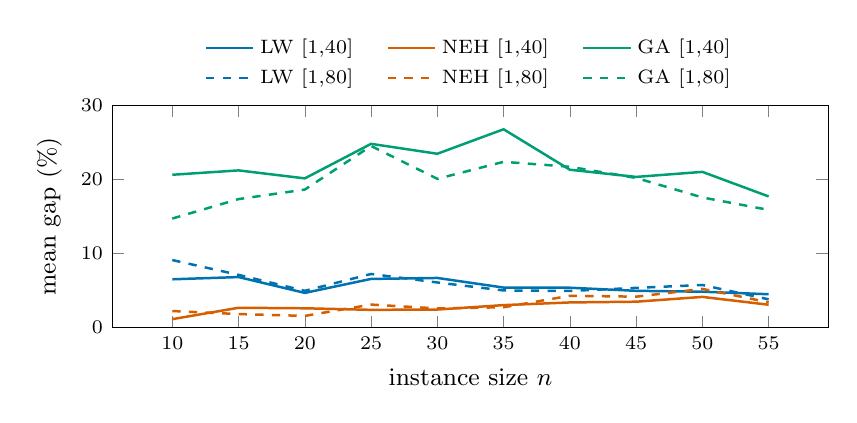
\begin{tikzpicture}
                \begin{axis}[
                    width=0.88\textwidth, height=4.4cm,
                    xlabel={instance size $n$}, ylabel={mean gap (\%)},
                    xtick={10,15,20,25,30,35,40,45,50,55}, xticklabels={10,15,20,25,30,35,40,45,50,55},
                    ymin=0, ymax=30,
                    tick label style={font=\scriptsize}, label style={font=\small},
                    every axis plot/.append style={line width=0.9pt},
                    legend columns=3,
                    legend style={font=\scriptsize, at={(0.5,1.03)}, anchor=south, draw=none,
                        /tikz/every even column/.append style={column sep=10pt}},
                    ]
                    \addplot[apxblue] coordinates {(10,6.50) (15,6.80) (20,4.66) (25,6.55) (30,6.68) (35,5.38) (40,5.36) (45,4.94) (50,4.82) (55,4.48)};
                    \addlegendentry{LW $[1{,}40]$}
                    \addplot[nehred] coordinates {(10,1.11) (15,2.65) (20,2.58) (25,2.37) (30,2.41) (35,3.01) (40,3.37) (45,3.47) (50,4.12) (55,3.06)};
                    \addlegendentry{NEH $[1{,}40]$}
                    \addplot[gagreen] coordinates {(10,20.63) (15,21.22) (20,20.14) (25,24.81) (30,23.47) (35,26.78) (40,21.31) (45,20.34) (50,21.02) (55,17.70)};
                    \addlegendentry{GA $[1{,}40]$}
                    \addplot[apxblue, dashed] coordinates {(10,9.10) (15,7.10) (20,4.94) (25,7.22) (30,6.07) (35,4.99) (40,4.92) (45,5.34) (50,5.73) (55,3.79)};
                    \addlegendentry{LW $[1{,}80]$}
                    \addplot[nehred, dashed] coordinates {(10,2.21) (15,1.80) (20,1.55) (25,3.08) (30,2.56) (35,2.72) (40,4.27) (45,4.15) (50,5.20) (55,3.39)};
                    \addlegendentry{NEH $[1{,}80]$}
                    \addplot[gagreen, dashed] coordinates {(10,14.71) (15,17.34) (20,18.63) (25,24.52) (30,20.08) (35,22.38) (40,21.71) (45,20.20) (50,17.56) (55,15.88)};
                    \addlegendentry{GA $[1{,}80]$}
                \end{axis}
            \end{tikzpicture}
            \caption{Small scale, weights $\in\{1,\ldots,100\}$.}
            \label{fig:gap-small-k100}
        \end{figure}

        \begin{table}[H]
            \resultstable
            \setlength{\tabcolsep}{6.74pt}
            \caption{Large scale, $p_{\max}=40$, weights $\in\{1,\ldots,30\}$}
            \label{tab:results-large-40}
            \begin{tabular}{@{}l r r r r @{\hspace{14pt}} r r r r @{\hspace{14pt}} r r r r@{}}
                \toprule
                \multirow{3}{*}{$n$} & \multicolumn{4}{c}{LW} & \multicolumn{4}{c}{NEH} & \multicolumn{4}{c}{GA} \\
                \cmidrule(lr){2-5}\cmidrule(lr){6-9}\cmidrule(lr){10-13}
                & \multicolumn{2}{c}{gap} & \multicolumn{2}{c}{time (ms)} & \multicolumn{2}{c}{gap} & \multicolumn{2}{c}{time (ms)} & \multicolumn{2}{c}{gap} & \multicolumn{2}{c}{time (ms)} \\
                \cmidrule(lr){2-3}\cmidrule(lr){4-5}\cmidrule(lr){6-7}\cmidrule(lr){8-9}\cmidrule(lr){10-11}\cmidrule(lr){12-13}
                & avg & max & avg & max & avg & max & avg & max & avg & max & avg & max \\
                \midrule
                $100$ & $\mathbf{4.4}$ & $10.0$ & $3.36\mathrm{e}{-2}$ & $6.16\mathrm{e}{-2}$ & $5.2$ & $9.7$ & $3.73\mathrm{e}1$& $6.30\mathrm{e}1$& $18.3$ & $29.2$ & $9.67\mathrm{e}2$& $1.10\mathrm{e}3$ \\
                $120$ & $\mathbf{3.5}$ & $6.5$ & $4.82\mathrm{e}{-2}$ & $1.05\mathrm{e}{-1}$ & $4.8$ & $10.0$ & $6.08\mathrm{e}1$& $6.32\mathrm{e}1$& $13.8$ & $32.1$ & $1.78\mathrm{e}3$& $1.85\mathrm{e}3$ \\
                $140$ & $\mathbf{3.0}$ & $6.6$ & $5.76\mathrm{e}{-2}$ & $1.19\mathrm{e}{-1}$ & $5.3$ & $8.5$ & $9.66\mathrm{e}1$& $1.03\mathrm{e}2$& $9.3$ & $20.6$ & $3.11\mathrm{e}3$& $3.20\mathrm{e}3$ \\
                $160$ & $\mathbf{3.4}$ & $7.5$ & $6.72\mathrm{e}{-2}$ & $1.28\mathrm{e}{-1}$ & $4.2$ & $7.4$ & $1.42\mathrm{e}2$& $1.47\mathrm{e}2$& $6.5$ & $14.4$ & $5.12\mathrm{e}3$& $5.29\mathrm{e}3$ \\
                $180$ & $\mathbf{2.6}$ & $7.8$ & $7.09\mathrm{e}{-2}$ & $9.77\mathrm{e}{-2}$ & $4.9$ & $7.6$ & $2.04\mathrm{e}2$& $2.15\mathrm{e}2$& $5.3$ & $13.8$ & $8.04\mathrm{e}3$& $8.37\mathrm{e}3$ \\
                $200$ & $\mathbf{2.6}$ & $5.6$ & $7.51\mathrm{e}{-2}$ & $1.17\mathrm{e}{-1}$ & $4.4$ & $7.6$ & $2.74\mathrm{e}2$& $2.89\mathrm{e}2$& $4.5$ & $15.7$ & $1.22\mathrm{e}4$& $1.26\mathrm{e}4$ \\
                $220$ & $3.4$ & $8.6$ & $8.67\mathrm{e}{-2}$ & $1.05\mathrm{e}{-1}$ & $5.0$ & $8.2$ & $3.64\mathrm{e}2$& $3.76\mathrm{e}2$& $\mathbf{3.0}$ & $11.7$ & $1.76\mathrm{e}4$& $1.84\mathrm{e}4$ \\
                $240$ & $\mathbf{2.8}$ & $5.9$ & $8.52\mathrm{e}{-2}$ & $1.11\mathrm{e}{-1}$ & $4.7$ & $7.3$ & $4.86\mathrm{e}2$& $5.08\mathrm{e}2$& $2.8$ & $7.4$ & $2.59\mathrm{e}4$& $2.69\mathrm{e}4$ \\
                $260$ & $2.6$ & $6.0$ & $9.98\mathrm{e}{-2}$ & $1.48\mathrm{e}{-1}$ & $5.4$ & $8.7$ & $5.69\mathrm{e}2$& $5.84\mathrm{e}2$& $\mathbf{1.6}$ & $4.7$ & $3.24\mathrm{e}4$& $3.29\mathrm{e}4$ \\
                $280$ & $2.5$ & $7.8$ & $9.67\mathrm{e}{-2}$ & $1.20\mathrm{e}{-1}$ & $5.1$ & $7.7$ & $7.22\mathrm{e}2$& $7.39\mathrm{e}2$& $\mathbf{0.8}$ & $3.9$ & $4.31\mathrm{e}4$& $4.37\mathrm{e}4$ \\
                $300$ & $2.0$ & $4.9$ & $1.11\mathrm{e}{-1}$ & $1.79\mathrm{e}{-1}$ & $4.9$ & $8.6$ & $8.99\mathrm{e}2$& $9.12\mathrm{e}2$& $\mathbf{0.9}$ & $5.0$ & $5.34\mathrm{e}4$& $5.45\mathrm{e}4$ \\
                $320$ & $3.0$ & $7.6$ & $1.13\mathrm{e}{-1}$ & $1.23\mathrm{e}{-1}$ & $4.4$ & $7.4$ & $1.10\mathrm{e}3$& $1.12\mathrm{e}3$& $\mathbf{1.2}$ & $6.3$ & $6.50\mathrm{e}4$& $6.59\mathrm{e}4$ \\
                $340$ & $1.5$ & $3.7$ & $1.27\mathrm{e}{-1}$ & $2.41\mathrm{e}{-1}$ & $4.7$ & $7.1$ & $1.32\mathrm{e}3$& $1.35\mathrm{e}3$& $\mathbf{1.2}$ & $8.0$ & $7.78\mathrm{e}4$& $7.89\mathrm{e}4$ \\
                $360$ & $2.2$ & $5.5$ & $1.31\mathrm{e}{-1}$ & $1.58\mathrm{e}{-1}$ & $4.7$ & $7.0$ & $1.58\mathrm{e}3$& $1.63\mathrm{e}3$& $\mathbf{0.9}$ & $7.1$ & $9.28\mathrm{e}4$& $9.61\mathrm{e}4$ \\
                $380$ & $2.3$ & $6.2$ & $1.36\mathrm{e}{-1}$ & $1.50\mathrm{e}{-1}$ & $4.5$ & $8.7$ & $1.87\mathrm{e}3$& $1.92\mathrm{e}3$& $\mathbf{0.3}$ & $1.5$ & $1.09\mathrm{e}5$& $1.11\mathrm{e}5$ \\
                $400$ & $2.0$ & $5.9$ & $1.46\mathrm{e}{-1}$ & $1.69\mathrm{e}{-1}$ & $3.9$ & $8.0$ & $2.18\mathrm{e}3$& $2.22\mathrm{e}3$& $\mathbf{0.6}$ & $2.7$ & $1.28\mathrm{e}5$& $1.30\mathrm{e}5$ \\
                \bottomrule
            \end{tabular}
        \end{table}

        \begin{table}[H]
            \resultstable
            \setlength{\tabcolsep}{6.74pt}
            \caption{Large scale, $p_{\max}=80$, weights $\in\{1,\ldots,30\}$}
            \label{tab:results-large-80}
            \begin{tabular}{@{}l r r r r @{\hspace{14pt}} r r r r @{\hspace{14pt}} r r r r@{}}
                \toprule
                \multirow{3}{*}{$n$} & \multicolumn{4}{c}{LW} & \multicolumn{4}{c}{NEH} & \multicolumn{4}{c}{GA} \\
                \cmidrule(lr){2-5}\cmidrule(lr){6-9}\cmidrule(lr){10-13}
                & \multicolumn{2}{c}{gap} & \multicolumn{2}{c}{time (ms)} & \multicolumn{2}{c}{gap} & \multicolumn{2}{c}{time (ms)} & \multicolumn{2}{c}{gap} & \multicolumn{2}{c}{time (ms)} \\
                \cmidrule(lr){2-3}\cmidrule(lr){4-5}\cmidrule(lr){6-7}\cmidrule(lr){8-9}\cmidrule(lr){10-11}\cmidrule(lr){12-13}
                & avg & max & avg & max & avg & max & avg & max & avg & max & avg & max \\
                \midrule
                $100$ & $\mathbf{3.6}$ & $8.9$ & $4.09\mathrm{e}{-2}$ & $1.25\mathrm{e}{-1}$ & $4.6$ & $10.8$ & $3.63\mathrm{e}1$& $4.12\mathrm{e}1$& $16.0$ & $30.1$ & $9.64\mathrm{e}2$& $1.02\mathrm{e}3$ \\
                $120$ & $\mathbf{4.4}$ & $12.9$ & $4.30\mathrm{e}{-2}$ & $7.13\mathrm{e}{-2}$ & $5.4$ & $9.3$ & $6.09\mathrm{e}1$& $6.21\mathrm{e}1$& $17.1$ & $38.5$ & $1.79\mathrm{e}3$& $1.85\mathrm{e}3$ \\
                $140$ & $\mathbf{3.5}$ & $10.7$ & $5.21\mathrm{e}{-2}$ & $9.38\mathrm{e}{-2}$ & $4.4$ & $7.7$ & $9.61\mathrm{e}1$& $9.95\mathrm{e}1$& $12.6$ & $25.3$ & $3.10\mathrm{e}3$& $3.24\mathrm{e}3$ \\
                $160$ & $\mathbf{3.2}$ & $11.4$ & $6.84\mathrm{e}{-2}$ & $1.12\mathrm{e}{-1}$ & $5.8$ & $9.9$ & $1.42\mathrm{e}2$& $1.51\mathrm{e}2$& $8.1$ & $25.8$ & $5.10\mathrm{e}3$& $5.23\mathrm{e}3$ \\
                $180$ & $\mathbf{3.0}$ & $7.3$ & $6.74\mathrm{e}{-2}$ & $9.56\mathrm{e}{-2}$ & $5.3$ & $9.0$ & $2.08\mathrm{e}2$& $2.50\mathrm{e}2$& $5.9$ & $14.3$ & $8.27\mathrm{e}3$& $8.55\mathrm{e}3$ \\
                $200$ & $\mathbf{2.7}$ & $8.6$ & $9.31\mathrm{e}{-2}$ & $2.55\mathrm{e}{-1}$ & $4.7$ & $7.2$ & $2.75\mathrm{e}2$& $2.88\mathrm{e}2$& $4.9$ & $10.1$ & $1.22\mathrm{e}4$& $1.26\mathrm{e}4$ \\
                $220$ & $\mathbf{2.9}$ & $8.0$ & $7.99\mathrm{e}{-2}$ & $1.12\mathrm{e}{-1}$ & $4.8$ & $8.7$ & $3.75\mathrm{e}2$& $3.97\mathrm{e}2$& $3.6$ & $9.0$ & $1.83\mathrm{e}4$& $1.93\mathrm{e}4$ \\
                $240$ & $2.9$ & $6.4$ & $8.86\mathrm{e}{-2}$ & $1.17\mathrm{e}{-1}$ & $6.0$ & $8.9$ & $4.55\mathrm{e}2$& $4.80\mathrm{e}2$& $\mathbf{1.9}$ & $6.5$ & $2.40\mathrm{e}4$& $2.54\mathrm{e}4$ \\
                $260$ & $1.8$ & $5.3$ & $9.07\mathrm{e}{-2}$ & $1.07\mathrm{e}{-1}$ & $5.2$ & $9.3$ & $5.71\mathrm{e}2$& $5.82\mathrm{e}2$& $\mathbf{1.6}$ & $8.0$ & $3.24\mathrm{e}4$& $3.32\mathrm{e}4$ \\
                $280$ & $2.3$ & $4.8$ & $1.02\mathrm{e}{-1}$ & $1.27\mathrm{e}{-1}$ & $5.5$ & $9.2$ & $7.22\mathrm{e}2$& $7.31\mathrm{e}2$& $\mathbf{0.8}$ & $4.3$ & $4.31\mathrm{e}4$& $4.38\mathrm{e}4$ \\
                $300$ & $2.8$ & $6.3$ & $1.03\mathrm{e}{-1}$ & $1.23\mathrm{e}{-1}$ & $5.4$ & $7.5$ & $8.98\mathrm{e}2$& $9.13\mathrm{e}2$& $\mathbf{2.0}$ & $11.8$ & $5.32\mathrm{e}4$& $5.41\mathrm{e}4$ \\
                $320$ & $1.9$ & $4.7$ & $1.21\mathrm{e}{-1}$ & $2.31\mathrm{e}{-1}$ & $5.7$ & $8.5$ & $1.10\mathrm{e}3$& $1.12\mathrm{e}3$& $\mathbf{1.4}$ & $6.1$ & $6.47\mathrm{e}4$& $6.62\mathrm{e}4$ \\
                $340$ & $1.4$ & $3.0$ & $1.19\mathrm{e}{-1}$ & $1.33\mathrm{e}{-1}$ & $5.6$ & $8.6$ & $1.33\mathrm{e}3$& $1.36\mathrm{e}3$& $\mathbf{0.8}$ & $3.3$ & $7.80\mathrm{e}4$& $7.97\mathrm{e}4$ \\
                $360$ & $1.7$ & $3.2$ & $1.27\mathrm{e}{-1}$ & $1.51\mathrm{e}{-1}$ & $5.8$ & $8.2$ & $1.58\mathrm{e}3$& $1.63\mathrm{e}3$& $\mathbf{1.1}$ & $7.3$ & $9.26\mathrm{e}4$& $9.39\mathrm{e}4$ \\
                $380$ & $1.8$ & $4.0$ & $1.37\mathrm{e}{-1}$ & $1.56\mathrm{e}{-1}$ & $5.9$ & $9.1$ & $1.87\mathrm{e}3$& $1.94\mathrm{e}3$& $\mathbf{0.8}$ & $2.9$ & $1.09\mathrm{e}5$& $1.13\mathrm{e}5$ \\
                $400$ & $1.7$ & $4.6$ & $1.48\mathrm{e}{-1}$ & $2.07\mathrm{e}{-1}$ & $5.8$ & $9.1$ & $2.19\mathrm{e}3$& $2.26\mathrm{e}3$& $\mathbf{0.8}$ & $2.9$ & $1.27\mathrm{e}5$& $1.29\mathrm{e}5$ \\
                \bottomrule
            \end{tabular}
        \end{table}

        \begin{figure}[H]
            \centering
            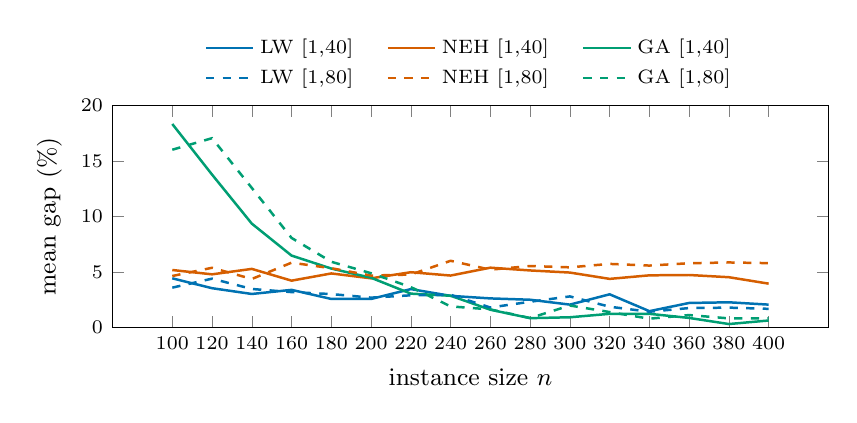
\begin{tikzpicture}
                \begin{axis}[
                    width=0.88\textwidth, height=4.4cm,
                    xlabel={instance size $n$}, ylabel={mean gap (\%)},
                    xtick={100,120,140,160,180,200,220,240,260,280,300,320,340,360,380,400}, xticklabels={100,120,140,160,180,200,220,240,260,280,300,320,340,360,380,400},
                    ymin=0, ymax=20,
                    tick label style={font=\scriptsize}, label style={font=\small},
                    every axis plot/.append style={line width=0.9pt},
                    legend columns=3,
                    legend style={font=\scriptsize, at={(0.5,1.03)}, anchor=south, draw=none,
                        /tikz/every even column/.append style={column sep=10pt}},
                    ]
                    \addplot[apxblue] coordinates {(100,4.42) (120,3.53) (140,3.01) (160,3.38) (180,2.56) (200,2.56) (220,3.45) (240,2.84) (260,2.61) (280,2.49) (300,2.05) (320,2.98) (340,1.46) (360,2.20) (380,2.26) (400,2.05)};
                    \addlegendentry{LW $[1{,}40]$}
                    \addplot[nehred] coordinates {(100,5.17) (120,4.78) (140,5.27) (160,4.21) (180,4.86) (200,4.42) (220,4.97) (240,4.67) (260,5.38) (280,5.13) (300,4.94) (320,4.37) (340,4.69) (360,4.72) (380,4.52) (400,3.94)};
                    \addlegendentry{NEH $[1{,}40]$}
                    \addplot[gagreen] coordinates {(100,18.33) (120,13.77) (140,9.35) (160,6.47) (180,5.30) (200,4.47) (220,3.04) (240,2.85) (260,1.59) (280,0.83) (300,0.91) (320,1.22) (340,1.22) (360,0.85) (380,0.30) (400,0.62)};
                    \addlegendentry{GA $[1{,}40]$}
                    \addplot[apxblue, dashed] coordinates {(100,3.58) (120,4.39) (140,3.46) (160,3.18) (180,3.00) (200,2.68) (220,2.89) (240,2.94) (260,1.79) (280,2.31) (300,2.79) (320,1.86) (340,1.41) (360,1.74) (380,1.78) (400,1.67)};
                    \addlegendentry{LW $[1{,}80]$}
                    \addplot[nehred, dashed] coordinates {(100,4.63) (120,5.37) (140,4.36) (160,5.83) (180,5.33) (200,4.67) (220,4.76) (240,6.00) (260,5.20) (280,5.53) (300,5.41) (320,5.72) (340,5.57) (360,5.78) (380,5.85) (400,5.79)};
                    \addlegendentry{NEH $[1{,}80]$}
                    \addplot[gagreen, dashed] coordinates {(100,16.01) (120,17.05) (140,12.57) (160,8.06) (180,5.91) (200,4.88) (220,3.63) (240,1.89) (260,1.62) (280,0.84) (300,1.97) (320,1.38) (340,0.78) (360,1.11) (380,0.81) (400,0.82)};
                    \addlegendentry{GA $[1{,}80]$}
                \end{axis}
            \end{tikzpicture}
            \caption{Large scale, weights $\in\{1,\ldots,30\}$.}
            \label{fig:gap-large}
        \end{figure}

        \begin{table}[H]
            \resultstable
            \setlength{\tabcolsep}{8.22pt}
            \caption{Large scale, $p_{\max}=40$, weights $\in\{1,\ldots,100\}$}
            \label{tab:results-large100-40}
            \begin{tabular}{@{}l r r r r @{\hspace{14pt}} r r r r @{\hspace{14pt}} r r r r@{}}
                \toprule
                \multirow{3}{*}{$n$} & \multicolumn{4}{c}{LW} & \multicolumn{4}{c}{NEH} & \multicolumn{4}{c}{GA} \\
                \cmidrule(lr){2-5}\cmidrule(lr){6-9}\cmidrule(lr){10-13}
                & \multicolumn{2}{c}{gap} & \multicolumn{2}{c}{time (ms)} & \multicolumn{2}{c}{gap} & \multicolumn{2}{c}{time (ms)} & \multicolumn{2}{c}{gap} & \multicolumn{2}{c}{time (ms)} \\
                \cmidrule(lr){2-3}\cmidrule(lr){4-5}\cmidrule(lr){6-7}\cmidrule(lr){8-9}\cmidrule(lr){10-11}\cmidrule(lr){12-13}
                & avg & max & avg & max & avg & max & avg & max & avg & max & avg & max \\
                \midrule
                $100$ & $\mathbf{4.0}$ & $10.6$ & $4.4\mathrm{e}{-2}$ & $9.6\mathrm{e}{-2}$ & $5.9$ & $9.6$ & $8.8\mathrm{e}1$ & $1.4\mathrm{e}2$ & $48.9$ & $76.5$ & $2.1\mathrm{e}3$ & $2.5\mathrm{e}3$ \\
                $120$ & $\mathbf{3.3}$ & $11.6$ & $6.5\mathrm{e}{-2}$ & $1.8\mathrm{e}{-1}$ & $5.6$ & $9.6$ & $1.4\mathrm{e}2$ & $1.7\mathrm{e}2$ & $48.0$ & $68.7$ & $4.1\mathrm{e}3$ & $4.7\mathrm{e}3$ \\
                $140$ & $\mathbf{2.9}$ & $8.8$ & $7.2\mathrm{e}{-2}$ & $3.0\mathrm{e}{-1}$ & $5.2$ & $9.1$ & $2.3\mathrm{e}2$ & $2.9\mathrm{e}2$ & $42.1$ & $63.9$ & $6.9\mathrm{e}3$ & $7.5\mathrm{e}3$ \\
                $160$ & $\mathbf{3.1}$ & $5.7$ & $8.8\mathrm{e}{-2}$ & $2.3\mathrm{e}{-1}$ & $5.6$ & $8.0$ & $3.0\mathrm{e}2$ & $4.3\mathrm{e}2$ & $45.1$ & $72.8$ & $1.1\mathrm{e}4$ & $1.2\mathrm{e}4$ \\
                $180$ & $\mathbf{3.5}$ & $7.6$ & $7.3\mathrm{e}{-2}$ & $1.9\mathrm{e}{-1}$ & $5.7$ & $9.4$ & $4.3\mathrm{e}2$ & $6.1\mathrm{e}2$ & $42.0$ & $57.8$ & $1.7\mathrm{e}4$ & $1.9\mathrm{e}4$ \\
                $200$ & $\mathbf{3.2}$ & $8.7$ & $8.3\mathrm{e}{-2}$ & $1.4\mathrm{e}{-1}$ & $6.1$ & $10.6$ & $6.3\mathrm{e}2$ & $8.4\mathrm{e}2$ & $42.2$ & $85.2$ & $2.6\mathrm{e}4$ & $2.8\mathrm{e}4$ \\
                $220$ & $\mathbf{2.5}$ & $6.2$ & $1.0\mathrm{e}{-1}$ & $1.5\mathrm{e}{-1}$ & $5.8$ & $9.0$ & $8.2\mathrm{e}2$ & $9.6\mathrm{e}2$ & $33.7$ & $44.3$ & $4.0\mathrm{e}4$ & $4.7\mathrm{e}4$ \\
                $240$ & $\mathbf{2.6}$ & $7.5$ & $1.2\mathrm{e}{-1}$ & $2.0\mathrm{e}{-1}$ & $5.9$ & $8.8$ & $1.0\mathrm{e}3$ & $1.3\mathrm{e}3$ & $31.9$ & $57.2$ & $5.5\mathrm{e}4$ & $5.8\mathrm{e}4$ \\
                $260$ & $\mathbf{2.8}$ & $5.0$ & $1.6\mathrm{e}{-1}$ & $3.1\mathrm{e}{-1}$ & $5.7$ & $7.9$ & $1.3\mathrm{e}3$ & $1.6\mathrm{e}3$ & $30.2$ & $46.2$ & $7.7\mathrm{e}4$ & $8.5\mathrm{e}4$ \\
                $280$ & $\mathbf{2.2}$ & $4.2$ & $1.5\mathrm{e}{-1}$ & $3.5\mathrm{e}{-1}$ & $6.1$ & $8.9$ & $1.9\mathrm{e}3$ & $2.6\mathrm{e}3$ & $26.6$ & $40.1$ & $1.2\mathrm{e}5$ & $1.6\mathrm{e}5$ \\
                $300$ & $\mathbf{2.2}$ & $4.9$ & $1.3\mathrm{e}{-1}$ & $2.6\mathrm{e}{-1}$ & $5.7$ & $8.6$ & $1.8\mathrm{e}3$ & $1.8\mathrm{e}3$ & $24.7$ & $37.0$ & $1.1\mathrm{e}5$ & $1.1\mathrm{e}5$ \\
                $320$ & $\mathbf{1.9}$ & $4.5$ & $1.7\mathrm{e}{-1}$ & $4.2\mathrm{e}{-1}$ & $5.1$ & $8.3$ & $2.2\mathrm{e}3$ & $2.3\mathrm{e}3$ & $23.2$ & $38.1$ & $1.3\mathrm{e}5$ & $1.4\mathrm{e}5$ \\
                $340$ & $\mathbf{1.6}$ & $3.2$ & $1.6\mathrm{e}{-1}$ & $2.8\mathrm{e}{-1}$ & $5.8$ & $8.0$ & $2.7\mathrm{e}3$ & $2.8\mathrm{e}3$ & $21.7$ & $34.7$ & $1.6\mathrm{e}5$ & $1.6\mathrm{e}5$ \\
                $360$ & $\mathbf{1.9}$ & $4.5$ & $1.6\mathrm{e}{-1}$ & $2.6\mathrm{e}{-1}$ & $5.7$ & $8.5$ & $3.2\mathrm{e}3$ & $3.3\mathrm{e}3$ & $17.5$ & $24.9$ & $1.9\mathrm{e}5$ & $1.9\mathrm{e}5$ \\
                $380$ & $\mathbf{1.7}$ & $5.6$ & $1.7\mathrm{e}{-1}$ & $2.6\mathrm{e}{-1}$ & $5.5$ & $8.9$ & $3.7\mathrm{e}3$ & $3.9\mathrm{e}3$ & $22.0$ & $39.6$ & $2.2\mathrm{e}5$ & $2.2\mathrm{e}5$ \\
                $400$ & $\mathbf{1.6}$ & $5.8$ & $1.7\mathrm{e}{-1}$ & $3.2\mathrm{e}{-1}$ & $5.3$ & $7.8$ & $4.3\mathrm{e}3$ & $4.4\mathrm{e}3$ & $19.3$ & $36.7$ & $2.5\mathrm{e}5$ & $2.6\mathrm{e}5$ \\
                \bottomrule
            \end{tabular}
        \end{table}

        \begin{table}[H]
            \resultstable
            \setlength{\tabcolsep}{8.22pt}
            \caption{Large scale, $p_{\max}=80$, weights $\in\{1,\ldots,100\}$}
            \label{tab:results-large100-80}
            \begin{tabular}{@{}l r r r r @{\hspace{14pt}} r r r r @{\hspace{14pt}} r r r r@{}}
                \toprule
                \multirow{3}{*}{$n$} & \multicolumn{4}{c}{LW} & \multicolumn{4}{c}{NEH} & \multicolumn{4}{c}{GA} \\
                \cmidrule(lr){2-5}\cmidrule(lr){6-9}\cmidrule(lr){10-13}
                & \multicolumn{2}{c}{gap} & \multicolumn{2}{c}{time (ms)} & \multicolumn{2}{c}{gap} & \multicolumn{2}{c}{time (ms)} & \multicolumn{2}{c}{gap} & \multicolumn{2}{c}{time (ms)} \\
                \cmidrule(lr){2-3}\cmidrule(lr){4-5}\cmidrule(lr){6-7}\cmidrule(lr){8-9}\cmidrule(lr){10-11}\cmidrule(lr){12-13}
                & avg & max & avg & max & avg & max & avg & max & avg & max & avg & max \\
                \midrule
                $100$ & $\mathbf{4.3}$ & $10.9$ & $3.8\mathrm{e}{-2}$ & $6.9\mathrm{e}{-2}$ & $5.3$ & $10.0$ & $8.1\mathrm{e}1$ & $1.1\mathrm{e}2$ & $50.7$ & $78.0$ & $2.2\mathrm{e}3$ & $2.5\mathrm{e}3$ \\
                $120$ & $\mathbf{4.4}$ & $13.1$ & $5.7\mathrm{e}{-2}$ & $9.8\mathrm{e}{-2}$ & $5.7$ & $11.8$ & $1.4\mathrm{e}2$ & $1.8\mathrm{e}2$ & $45.8$ & $75.3$ & $4.0\mathrm{e}3$ & $4.4\mathrm{e}3$ \\
                $140$ & $\mathbf{3.1}$ & $8.3$ & $7.6\mathrm{e}{-2}$ & $2.4\mathrm{e}{-1}$ & $6.2$ & $10.2$ & $2.2\mathrm{e}2$ & $3.4\mathrm{e}2$ & $44.5$ & $69.1$ & $7.0\mathrm{e}3$ & $7.5\mathrm{e}3$ \\
                $160$ & $\mathbf{3.0}$ & $8.0$ & $7.7\mathrm{e}{-2}$ & $1.4\mathrm{e}{-1}$ & $5.0$ & $7.7$ & $3.0\mathrm{e}2$ & $3.5\mathrm{e}2$ & $38.9$ & $56.4$ & $1.1\mathrm{e}4$ & $1.2\mathrm{e}4$ \\
                $180$ & $\mathbf{3.2}$ & $7.0$ & $8.0\mathrm{e}{-2}$ & $2.3\mathrm{e}{-1}$ & $5.9$ & $11.1$ & $4.3\mathrm{e}2$ & $7.8\mathrm{e}2$ & $40.5$ & $61.4$ & $1.7\mathrm{e}4$ & $1.9\mathrm{e}4$ \\
                $200$ & $\mathbf{3.4}$ & $7.2$ & $1.1\mathrm{e}{-1}$ & $3.3\mathrm{e}{-1}$ & $6.7$ & $9.9$ & $6.3\mathrm{e}2$ & $1.1\mathrm{e}3$ & $37.1$ & $49.3$ & $2.7\mathrm{e}4$ & $3.2\mathrm{e}4$ \\
                $220$ & $\mathbf{3.0}$ & $7.0$ & $1.2\mathrm{e}{-1}$ & $2.4\mathrm{e}{-1}$ & $6.5$ & $9.5$ & $8.2\mathrm{e}2$ & $1.0\mathrm{e}3$ & $35.0$ & $59.2$ & $3.9\mathrm{e}4$ & $4.2\mathrm{e}4$ \\
                $240$ & $\mathbf{2.4}$ & $5.5$ & $1.1\mathrm{e}{-1}$ & $2.0\mathrm{e}{-1}$ & $7.3$ & $10.1$ & $9.9\mathrm{e}2$ & $1.1\mathrm{e}3$ & $33.4$ & $58.6$ & $5.5\mathrm{e}4$ & $5.9\mathrm{e}4$ \\
                $260$ & $\mathbf{2.3}$ & $5.6$ & $1.3\mathrm{e}{-1}$ & $3.0\mathrm{e}{-1}$ & $6.3$ & $9.7$ & $1.4\mathrm{e}3$ & $2.3\mathrm{e}3$ & $27.1$ & $45.4$ & $8.6\mathrm{e}4$ & $1.2\mathrm{e}5$ \\
                $280$ & $\mathbf{1.7}$ & $5.0$ & $1.4\mathrm{e}{-1}$ & $2.2\mathrm{e}{-1}$ & $6.6$ & $9.5$ & $1.8\mathrm{e}3$ & $2.6\mathrm{e}3$ & $27.3$ & $50.3$ & $1.1\mathrm{e}5$ & $1.4\mathrm{e}5$ \\
                $300$ & $\mathbf{2.7}$ & $6.1$ & $1.4\mathrm{e}{-1}$ & $2.1\mathrm{e}{-1}$ & $6.8$ & $9.9$ & $1.8\mathrm{e}3$ & $1.8\mathrm{e}3$ & $28.7$ & $40.8$ & $1.1\mathrm{e}5$ & $1.1\mathrm{e}5$ \\
                $320$ & $\mathbf{2.4}$ & $6.0$ & $1.4\mathrm{e}{-1}$ & $2.5\mathrm{e}{-1}$ & $6.7$ & $10.4$ & $2.3\mathrm{e}3$ & $2.3\mathrm{e}3$ & $24.7$ & $33.1$ & $1.3\mathrm{e}5$ & $1.3\mathrm{e}5$ \\
                $340$ & $\mathbf{2.1}$ & $4.1$ & $2.2\mathrm{e}{-1}$ & $1.5\mathrm{e}0$ & $6.5$ & $9.3$ & $2.7\mathrm{e}3$ & $2.8\mathrm{e}3$ & $22.9$ & $38.5$ & $1.6\mathrm{e}5$ & $1.6\mathrm{e}5$ \\
                $360$ & $\mathbf{2.4}$ & $5.6$ & $1.9\mathrm{e}{-1}$ & $3.5\mathrm{e}{-1}$ & $7.6$ & $10.0$ & $3.2\mathrm{e}3$ & $3.4\mathrm{e}3$ & $21.3$ & $40.3$ & $1.9\mathrm{e}5$ & $1.9\mathrm{e}5$ \\
                $380$ & $\mathbf{1.7}$ & $5.3$ & $1.8\mathrm{e}{-1}$ & $2.7\mathrm{e}{-1}$ & $5.5$ & $8.5$ & $3.7\mathrm{e}3$ & $3.8\mathrm{e}3$ & $18.5$ & $37.0$ & $2.2\mathrm{e}5$ & $2.2\mathrm{e}5$ \\
                $400$ & $\mathbf{2.0}$ & $4.5$ & $2.0\mathrm{e}{-1}$ & $3.6\mathrm{e}{-1}$ & $6.6$ & $9.0$ & $4.2\mathrm{e}3$ & $4.4\mathrm{e}3$ & $18.6$ & $30.6$ & $2.6\mathrm{e}5$ & $2.7\mathrm{e}5$ \\
                \bottomrule
            \end{tabular}
        \end{table}

        \begin{figure}[H]
            \centering
            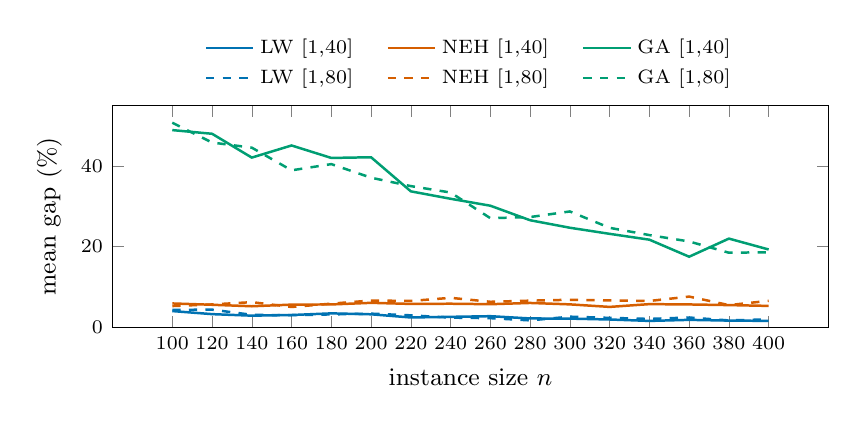
\begin{tikzpicture}
                \begin{axis}[
                    width=0.88\textwidth, height=4.4cm,
                    xlabel={instance size $n$}, ylabel={mean gap (\%)},
                    xtick={100,120,140,160,180,200,220,240,260,280,300,320,340,360,380,400}, xticklabels={100,120,140,160,180,200,220,240,260,280,300,320,340,360,380,400},
                    ymin=0, ymax=55,
                    tick label style={font=\scriptsize}, label style={font=\small},
                    every axis plot/.append style={line width=0.9pt},
                    legend columns=3,
                    legend style={font=\scriptsize, at={(0.5,1.03)}, anchor=south, draw=none,
                        /tikz/every even column/.append style={column sep=10pt}},
                    ]
                    \addplot[apxblue] coordinates {(100,4.04) (120,3.28) (140,2.90) (160,3.06) (180,3.47) (200,3.24) (220,2.45) (240,2.61) (260,2.77) (280,2.21) (300,2.17) (320,1.95) (340,1.60) (360,1.86) (380,1.68) (400,1.61)};
                    \addlegendentry{LW $[1{,}40]$}
                    \addplot[nehred] coordinates {(100,5.93) (120,5.60) (140,5.23) (160,5.64) (180,5.68) (200,6.08) (220,5.81) (240,5.86) (260,5.74) (280,6.05) (300,5.70) (320,5.07) (340,5.76) (360,5.68) (380,5.52) (400,5.32)};
                    \addlegendentry{NEH $[1{,}40]$}
                    \addplot[gagreen] coordinates {(100,48.89) (120,47.98) (140,42.08) (160,45.08) (180,41.99) (200,42.16) (220,33.71) (240,31.87) (260,30.15) (280,26.55) (300,24.69) (320,23.18) (340,21.73) (360,17.51) (380,22.00) (400,19.30)};
                    \addlegendentry{GA $[1{,}40]$}
                    \addplot[apxblue, dashed] coordinates {(100,4.34) (120,4.39) (140,3.11) (160,3.02) (180,3.21) (200,3.40) (220,2.98) (240,2.41) (260,2.28) (280,1.73) (300,2.65) (320,2.35) (340,2.10) (360,2.44) (380,1.72) (400,1.99)};
                    \addlegendentry{LW $[1{,}80]$}
                    \addplot[nehred, dashed] coordinates {(100,5.28) (120,5.68) (140,6.25) (160,5.05) (180,5.88) (200,6.65) (220,6.55) (240,7.32) (260,6.34) (280,6.62) (300,6.84) (320,6.68) (340,6.54) (360,7.63) (380,5.52) (400,6.57)};
                    \addlegendentry{NEH $[1{,}80]$}
                    \addplot[gagreen, dashed] coordinates {(100,50.73) (120,45.81) (140,44.54) (160,38.92) (180,40.46) (200,37.09) (220,35.01) (240,33.42) (260,27.06) (280,27.34) (300,28.73) (320,24.67) (340,22.87) (360,21.29) (380,18.50) (400,18.62)};
                    \addlegendentry{GA $[1{,}80]$}
                \end{axis}
            \end{tikzpicture}
            \caption{Large scale, weights $\in\{1,\ldots,100\}$.}
            \label{fig:gap-large-k100}
        \end{figure}

        \section{Conclusion} \label{sec:conclusion}

        The maximum weighted completion time problem has a simple optimal rule on a single machine: jobs are scheduled in non-increasing order of weight. In a two-machine flow shop, however, a job's completion time depends on its position in the sequences processed on both machines, making the problem substantially more challenging.
        This paper studied the two-machine problem, $F2 \mid \mid WC_{\max}$, to identify the structural properties of optimal schedules and the algorithmic guarantees they enable.

        We first established that the problem is binary $\mathcal{NP}$-hard even with only two distinct weights, and strongly $\mathcal{NP}$-hard when the number of distinct weights is unrestricted.
        We then showed that an optimal schedule consists of weight-based blocks ordered by non-increasing weight, with jobs within each block arranged according to Johnson's rule.
        This structure provides the basis for an exact $DP$ that eliminates dominated states, an $FPTAS$ for a fixed number of distinct weights, and the $LW$ rule.
        For larger instances, we adapted the $NEH$ heuristic and developed a weight-block $GA$, and compared all these methods with the $MILP$ model.

        The structural and computational limitations identified in this study motivate several directions for future research.
        First, both the block structure and the $DP$ are developed for two machines. Extending the problem to an arbitrary number of machines requires investigating whether the block structure and ordering properties can be preserved, and how the role of Johnson's rule changes.
        Second, the running time of the $DP$ grows rapidly with the number of distinct weight values, leaving some instances, such as those with 140 jobs under the wider processing-time range, unsolved. Whether a branch-and-bound algorithm can solve such instances more effectively remains an open question.
        Third, the heuristics considered here rely on manually designed rules and operators. Reinforcement learning, particularly Q-learning, could be used to learn dispatching rules for this objective or to guide the mutation and crossover operators of $GA$, potentially improving their adaptability to instance families not known in advance.
        More broadly, these results provide a structural foundation for developing exact and heuristic methods for weighted bottleneck objectives in flow shops.
                
        \bibliographystyle{apalike}
        \bibliography{ref-shop}
        
    \end{sloppypar}
\end{document}

